\documentclass[12pt]{article}
\usepackage{makeidx}
\usepackage{multirow}
\usepackage{multicol}
\usepackage[dvipsnames,svgnames,table]{xcolor}
\usepackage{graphicx}
\usepackage{ulem}
\usepackage[linktoc=none]{hyperref}
\usepackage{alltt}

% Needed by Maryam
\usepackage{amsmath} 
\usepackage{amssymb} 
\usepackage{amsthm}
\usepackage{amsfonts}
\usepackage{subfigmat}


%\author{Claire Tomlin, Christopher Brooks, UC Berkeley}
\author{Lots of Folks, adapted from LaTeX code by Claire and Christopher}
\title{Multi-University Research Initiative on High-Confidence Design for Distributed Embedded Systems}



\makeatletter
\newenvironment{indentation}[3]%
	       {\par\setlength{\parindent}{#3}
	         \setlength{\leftmargin}{#1}       \setlength{\rightmargin}{#2}%
	         \advance\linewidth -\leftmargin       \advance\linewidth -\rightmargin%
	         \advance\@totalleftmargin\leftmargin  \@setpar{{\@@par}}%
	         \parshape 1\@totalleftmargin \linewidth\ignorespaces}{\par}%
               \makeatother 

               % new LaTeX commands
               \newcommand{\styleAbstract}[1]{#1}
               \newcommand{\styleAbstractChar}[1]{#1}
               \newcommand{\styleAbstractCharOne}[1]{#1}
               \newcommand{\styleAchievement}[1]{{\footnotesize \textsf{#1}}}
               \newcommand{\styleBody}[1]{#1}
               \newcommand{\styleBodyTextChar}[1]{#1}
               \newcommand{\styleBulleted}[1]{#1}
               \newcommand{\styleContributions}[1]{#1}
               \newcommand{\stylepapertitle}[1]{#1}
               \newcommand{\styleSubsubtopic}[1]{\textit{\uline{#1}}}
               \newcommand{\styleSubtopic}[1]{\uline{#1}}
               \newcommand{\styleTopic}[1]{\textbf{\textit{#1}}}
               \newcommand{\styleTopicChar}[1]{\textbf{\textit{#1}}}

               \begin{document}
% Front Page

                \begin{center}
                 \begin{indentation}{0pt}{0pt}{0pt}
                   \textbf{{\large Multi-University Research Initiative on \\
                       High-Confidence Design for Distributed Embedded Systems}}
                 \end{indentation}
               \end{center}

               \begin{center}
                 \begin{indentation}{0pt}{0pt}{0pt}

                 \end{indentation}
               \end{center}

               \begin{center}
                 \begin{indentation}{0pt}{0pt}{0pt}
                   {\LARGE Frameworks and Tools for \\
                       High-Confidence Design of Adaptive, \\
                       Distributed Embedded Control Systems}
                 \end{indentation}
               \end{center}

               \begin{center}
                 \begin{indentation}{0pt}{0pt}{0pt}
                   \textbf{{\large Final Report}}
                 \end{indentation}
               \end{center}

               \begin{center}
                 \begin{indentation}{0pt}{0pt}{0pt}

                 \end{indentation}
               \end{center}

               \begin{center}
                 \begin{indentation}{0pt}{0pt}{0pt}
                 \end{indentation}
               \end{center} 

               \begin{center}
                 \begin{indentation}{0pt}{0pt}{0pt}
                 \end{indentation}
               \end{center} 

               \begin{center}
                 \begin{indentation}{0pt}{0pt}{0pt}
                 { Vanderbilt University \\
                   Institute for Software Integrated Systems \\
                   1025 16th Avenue South, Suite 102, Nashville, TN 37212 \\
                   (615) 322-3455 (office) \\
                   (615) 343-7440 (fax) \\
                   \underline{janos.sztipanovits@vanderbilt.edu} }
                 \end{indentation}
               \end{center}              

               \begin{center}
                 \begin{indentation}{0pt}{0pt}{0pt}
                 \end{indentation}
               \end{center}               

                \begin{center}
                 \begin{indentation}{0pt}{0pt}{0pt}
                 {TEAM MEMBERS}
                 \end{indentation}
               \end{center}

               \begin{center}
                 \begin{indentation}{0pt}{0pt}{0pt}

                 \end{indentation}
               \end{center}

                \begin{center}
                 \begin{indentation}{0pt}{0pt}{0pt}
                { \textbf{Vanderbilt:} J. Sztipanovits (PI) and G. Karsai \\
                  \textbf{UC Berkeley:} C. Tomlin (Lead and Co-PI), Edward Lee, and S. Sastry \\
                  \textbf{CMU:} Bruce Krogh (Lead and Co-PI) and Edmund Clarke \\
                  \textbf{Stanford:} Stephen Boyd }
                 \end{indentation}
               \end{center}


               \begin{center}
                 \begin{indentation}{0pt}{0pt}{0pt}
                 \end{indentation}
               \end{center} 

               \begin{center}
                 \begin{indentation}{0pt}{0pt}{0pt}
                 \end{indentation}
               \end{center} 

               \begin{center}
                 \begin{indentation}{0pt}{0pt}{0pt}
                 FA-9550-06-0312
                 \end{indentation}
               \end{center} 


               \pagebreak{}

               \tableofcontents

               \pagebreak{}



               \pagebreak

               \section{High-Confidence Design for Distributed Embedded Systems (HCDDES) MURI}

               The Multidisciplinary University Research Initiative
               (MURI) project on High-Confidence Design for
               Distributed Embedded Systems integrate verification,
               validation, and test procedures throughout the complete
               design, development and maintenance cycle, from
               requirements capture to deployment and life cycle
               updates. 
               
               This project was funded by the Air Force Office
               of Scientific Research.  The project started with a kickoff meeting on August 7, 2006 and on August 31, 2011.

The design of embedded systems is challenging for high-confidence aerospace systems, where technology leadership is the key to superiority. Next generation unmanned air vehicles (UAVs) and space vehicles (SVs) are complex systems of systems involving multiple synchronous and asynchronous processes in an architecture distributed across several processors both within a single UAV (SV) and across groups of UAVs (SVs). Additionally, autonomy, fault tolerance, and resource optimization require that mixed-criticality functions are resident on the same processors in this architecture. Guaranteeing the provably correct behavior of the overall embedded system is extremely difficult, especially with respect to timing constraints and their relationship to safety of the physical systems, and performance specifications associated with mission-level objectives. Traditional software engineering methods cannot solve these problems because they do not address properties key to the interaction of physical processes with software, such as timing, mixed criticality functions, and concurrent processes.

%This project developed a comprehensive approach to the design of high-confidence complex embedded systems, that is, systems that are correct-by-construction, fault tolerant, secure, and degrade gracefully under fault conditions or information attack. Our approach integrates verification, validation, and test procedures throughout the complete design, development and maintenance cycle, from requirements capture to deployment and life cycle updates. This MURI project had the following research areas:

%               \begin{enumerate}
%               \item Hybrid and embedded systems theory.
%               \item Model-based software design/verification.
%               \item Composable Tool Architectures.
%              \item Testing and Experimental Validation. 
%               \end{enumerate}
               
%	      At Berkeley, the participating faculty were Claire Tomlin, S. Shankar Sastry and Edward A. Lee.
	      
%               This report contains Berkeley's year 5 input (key achievements, publications, management
%               related data) in an overview style that lists the key
%               results of the last year and during the project.



\section{Objectives}

This project aims to develop a comprehensive approach to the model-based design of high-confidence distributed embedded systems. We take advantage and fully leverage a shared theoretical foundation and technology infrastructure in four focus areas: hybrid and embedded systems theory, model-based software design, composable tool architectures and experimental testbeds. The objectives of our research in the focus areas are the following:   

\begin{enumerate}

\item Develop theory of deep composition of hybrid systems with attributes of computational and communication platforms. We address compositionality, concurrency, heterogeneity and resource constraints, robustness, approximate verification, and adaptive control architectures for uncertainty handling.

\item Develop foundations of model-based software design for high-confidence, networked embedded systems applications. We investigate new semantic foundations for modeling languages and model transformations, precisely architected software and systems platforms that guarantee system properties via construction, and new methods for static source code verification and testing, as well as for dynamic runtime verification and testing.

\item Develop composable tool architectures that supports high-level reusability of modeling, model analysis, verification, and testing tools in domain-specific tool chains. We create new foundations for tool integration that go beyond data modeling and data transfer.

\item Demonstrate the overall effort by creating an end-to-end design tool chain prototype for model-based generation and verification of embedded controller code for experimental platforms.

\end{enumerate}



              % \section{Status of Effort}
	     
               \section{Accomplishments and New Findings}

               
\subsection{Hybrid and Embedded Systems Theory} 

            %\subsubsection{Finite State Machines and Modal Models (Lee)}

            %Finite State Machines and Modal Models in Ptolemy II Finite-state machines (FSMs) and modal models provide a very expressive way to build up complex model behaviors. As a consequence of this expressiveness, it takes some practice to learn to use them well. Edward Lee has compiled a technical memorandum \cite{Lee:EECS-2009-151} that describes the usage and semantics of FSMs and modal models in Ptolemy II. 

            %FSMs are actors whose behavior is described using a finite set of states and transitions be-tween the states. The transitions between the states are enabled by guards, which are boolean-valued expressions that can reference inputs to the actor and parameters in scope. The transitions can produce outputs and can update the value of parameters in scope. Modal models extend FSMs by allowing states to have refinements, which are hierarchical Ptolemy II models. The re-finements may themselves be FSMs, modal models, or any composite actor containing a director compatible with the domain in which the modal model is being used. On the basis of several ex-amples, the memorandum describes the operational semantics, the practical usage, and the se-mantics of time in modal models. 

            %Each of the figures in the document corresponds to an executable Ptolemy II model. To exe-cute and experiment with these models the reader can simply click on the corresponding figures in the document. There is no need to pre-install Ptolemy II or any other software. 

            \subsubsection{Constructive Architectures for Digital Controllers of Continuous Time Systems (Kottenstette)}

Our overall research goal has been to create constructive networked control architectures for formation control of both quadrotor and fixed-wing aircraft which allows for collision avoidance while maintaining stability.  In order to obtain this goal we: 1) developed a constructive non-linear control framework which allows non-linear affine systems such as fixed-wing aircraft to be rendered strictly-output passive; 2) established a networked control architecture to interconnect multiple-agents in order to achieve a formation; and 3) modified a classic collision avoidance algorithm in order to achieve separation of aircraft.

\begin{enumerate}
\item Our first result applies to networked control of non-linear affine systems, including fixed wing aircraft, quadrotor aircraft, robotic, thermal, semiconductor manufacturing, alternative energy generation, and active suspension systems. These nonlinear affine systems can be expressed through what we term "m-Triangular Systems". The m-Triangular System renders possible a well-posed, distributed, continuous-time, control law which can be applied to nonlinear affine systems. This control law creates a strictly-output passive system which can then be integrated into a multirate discrete time networked control architecture. This robust architecture permits a discrete time strictly passive lag compensator to determine the desired output of the strictly-output passive system. Thus, we can integrate unmanned jet fighter aircraft into the NextGen system in which the lag compensator is located at the ground-control station. We can now safely control the inertial position of these aircraft despite communication time varying delays and data loss \cite{NK_1a,NK_1b,NK_1c}.
\item Our second result builds on our advanced digital networked control architecture in which passivity is preserved in spite time varying delays and data loss \cite{NK_2}.  The key to this architecture is our networking abstraction known as the power-junction and some minor analysis showing that it can be distributed over arbitrary overlay network topologies \cite{NK_3a,NK_3b}.  The overall architecture then allows for steady-state analysis in order to derive final formations of quadrotor aircraft.  These predicted results have been verified using our advanced Simulink based models of quadrotor aircraft in which time varying delays and data loss were simulated using TrueTime.  
\item Finally the classical collision avoidance algorithms \cite{NK_4a,NK_4b} had to be modified using a non-linear filtering architecture which is described precisely in \cite{NK_1a} and filtering architecture is inspired on the pioneering work of \cite{NK_5a,NK_5b,NK_5c}.
\end{enumerate}


            We have recently demonstrated how to interconnect either a linear or nonlinear interior-conic continuous time systems (in which passive systems are a special case) to an appropriately constrained conic digital controller in which continuous time stability ($L_m^2$-stability) can be guaranteed in spite of time-varying delay.  The key to achieving a stronger result and further weaken our initial passivity assumptions of the continuous time system is to explicitly consider the resulting conic-system properties resulting from the feedback loops created from our use of wave variables.  Initial results demonstrate improved rejection of high-frequency noise which can be effectively filtered with multi-rate passive samplers (PS:MTs) and passive hold devices (PH:M Ts) while achieving better performance over traditional sample-and-hold digital control systems.  As a result, we can now control the position of robotic arm manipulators using direct position feedback instead of indirect velocity feedback.  In addition we have shown that the inner-product-equivalent sampler and zero-order-hold (IPESH) not only preserves passivity properties of a given system but preserves the more general interior-conic system properties as well.  The implication is that like the bilinear-transform which preserves both passivity and stability properties when mapping a continuous linear time invariant (LTI) system to a discrete LTI system, the IPESH in general preserves stability for nonlinear interior conic systems such that if the IPESH is applied to a continuous interior conic system which is inside the sector $[a,b]$ then the resulting discrete-time system whose output is scaled by $\frac{1}{T_s}$) remains inside the sector $[a,b]$.  These results should extend to those related to control over power junction networks.

            We have demonstrated that a simplified linear power junction network can be used in distributed deployment of point-mass systems whose inertial position control system closely resembles that used to control position for our quadrotor aircraft.  Furthermore a resilient power junction network has also been demonstrated to allow a single plant to be reliably controlled by many redundant digital controllers in order to better withstand both denial-of-service (DOS) attacks and even safely handle certain compromises of the redundant controllers.  The linear power junction network appears to be a good candidate for networked control of quadrotor aircraft as well as fixed wing aircraft.

    In order to better study formation control of fixed wing aircraft for a potential aerial refueling scenario posed at our 2009 review we had to develop an inertial control system and model of a fixed wing aircraft.  Therefore we developed and verified an advanced Simulink-based fixed wing model of the Cessna A-37 whose velocity flight path and heading angles were maintained by a resilient backstepping control law.  The backstepping control law was derived using a simplifying small-angle assumption involving the angle of attack and bank angle while maintaining the side-slip angle near zero.  It achieves performance close to its adaptive counterparts while allowing for system model verification.  In addition we demonstrated that if we filter one of the feedback terms typically required to achieve asymptotic stability results for our backstepping controller then we could better withstand discrete time wind gusts.  In general we proved our backstepping control law can be applied not only to the control of fixed wing aircraft but other nonlinear systems which possess triangular structures and invertible controller affine terms.  Finally we demonstrated that a classical anti-windup compensator can be applied to the velocity control system when subject to control thrust saturation which can occur during aggressive maneuvers.  The small-angle assumption allowed us to significantly simplify our backstepping control law for our fixed wing aircraft, however, the quadrotor aircraft control system was still much less complicated.  Although both systems share the same kinematic equations of motion, the fixed wing aircraft dynamics depend heavily on the wind velocity vector.  As a result it is not clear how to exploit the passivity-like subsystems related to the kinematics in order to simplify the control design as was done for the quadrotor aircraft.  However, one technique to simplify controller design which looks promising is Interconnection Damping Assignment Passivity Based Control (IDA-PBC).

    IDA-PBC attempts to derive control laws which attempt to exploit the passivity-like properties of a system in order to derive a dissipative structure which achieves asymptotic stability.  Unlike backstepping control laws, IDA-PBC is not as aggressive in attempting to cancel non-linear terms in the system in order to make it appear as a cascade of integrators.  As a result the IDA-PBC control laws are typically less computationally intensive and possess more linear feedback terms similar to those seen with our quadrotor control system. We have studied, implemented and refined an IDA-PBC control algorithm initially presented by Johnsen \& Allgower related to the control of a four-tank process.  We have developed preliminary tools to automatically generate IDA-PBCs while providing improved integrator anti-windup compensators.  Furthermore we determined that the bilinear-transform works quite well in implementing low-sample-rate (possibly nonlinear) integrator terms in the IDA-PB controllers.  Furthermore IDA-PBC allows us to determine explicit gain and trajectory constraints to apply to our controller implementation in order to further improve system resilience.

\subsubsection{Robust Group Coordination}

For many sensing, surveillance, or tracking applications, it is often desirable to deploy a group of unmanned aerial vehicles (UAVs) for reconnaissance or scouting using coordination algorithms for decentralized control. Using large numbers of UAVs equipped with surveillance and sensing equipment is beneficial because redundancy reduces the likelihood of missing interesting events in the presence of obstructions caused by non-uniform terrain, man-made structures, or man-made interference. Therefore, we aim to develop methods that utilize decentralized control of UAVs to enhance security and redundancy for group coordination problems.

Performing coordinated tasks such as establishing a formation or output synchronization requires local interactions (e.g., via message passing) in a discrete-time framework for multi-agent systems. However network uncertainties such as delays and dropped packets introduce additional challenges to achieving the desired task. In particular, stability of the networked system can be jeopardized by these effects.  To circumvent the stability problems caused by the discrete-time implementation of multi-agent networks, a compositional approach has been created using passivity, which ensures $l_m^2$-stability of the global system whenever the individual components are passive.  Specifically, we have created and implemented an inherently distributed and passive communication architecture, which allows strictly-output passive, dynamical systems to be coupled through any discrete time overlay network in a stability-preserving manner, regardless of time-varying delays and data loss.

The specific problem we consider for our application of the passive communication architecture is the situation where $n$ agents distributed randomly in a two-dimensional environment attempt to create a formation surrounding a target position. Each agent has a neighborhood within which it is able to communicate, and no information is shared globally.

Fig. \ref{fig:consensus_3nodes} presents an example three node neighborhood communication scheme between nodes $i$, $j$, and $q$.  Each node sends position information encoded as a wave variable $u(k)$ to a delay state $d(k)$. The delay state passes the delayed information $v(k)$ as an input to the corresponding node.  The entire scenario is made of collections of these neighborhoods that have overlapping nodes.

               \begin{figure}[thpb]
 	         \centering
	         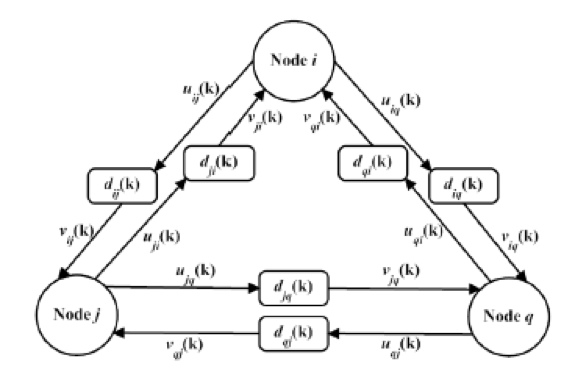
\includegraphics[width=0.9\textwidth]{img/consensus_3nodes}
	         \caption{An example 3-node communication network, illustrating the delay terminology.}
	         \label{fig:consensus_3nodes}
               \end{figure}



We have developed and tested (in simulation) the decentralized passivity and coordination algorithms for multiple UAV formation control.   We verified that the algorithms perform well in the presence of communication delays and dropouts, and have been shown to work well for systems even in the presence of large communication loss or delays.

               \begin{figure}[thpb]
 	         \centering
	         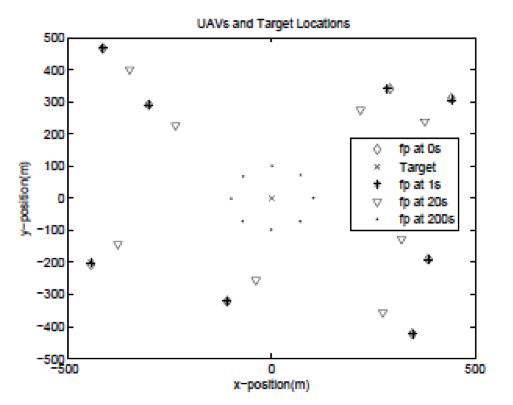
\includegraphics[width=0.9\textwidth]{img/consensus_sim}
	         \caption{Progression of UAVs to desired locations in presence of 10\% packet loss.}
	         \label{fig:consensus_sim}
               \end{figure}



One of our experimental scenarios involved a network of eight UAVs distributed in a regular lattice network structure.  Each UAV has four neighbors that it can communicate with using our passivity framework over the network, and we modeled a 10\% probability of packet loss. The scenario was modeled using Matlab and TrueTime for network communication simulation.  Fig. \ref{fig:consensus_sim} presents snapshots of the UAV positions at various times during the simulation.  It can be seen that the UAVs end up surrounding the target in the desired formation even with the network interference

            \subsubsection{Hierarchies of Robust Hybrid and Embedded Systems (Tomlin, Krogh, Sastry)} 
               
               \textit{Reachability Analysis.}  In safety-critical
               applications, the task of controller design and
               synthesis is often subject to hard constraints such as
               safe operation envelopes, target attainability
               requirements, and limits on the admissible control
               inputs.  Furthermore, due to various uncertainties in
               the modeling phase and operation phase, the controller
               design must be robust to factors such as modeling
               error, environment disturbances, and adversarial
               actions.

               Over the course of this MURI, we have developed several
               methods for addressing these problems in the context of
               a hybrid system abstraction, which is a powerful
               modeling framework encapsulating both continuous and
               discrete dynamics.  Our approach is based upon a
               dynamic game formulation of reachability analysis in
               which the safety and target attainability objectives
               are encoded as reachability objectives, and the
               disturbance is modelled as an adversarial agent.  In
               the following, we will briefly outline some of these
               methods, along with relevant application scenarios.

               \emph{a) Provably Safe Maneuver Sequence Design}

               In the case where the sequence of transitions in a
               hybrid system is known ahead of time, we have developed
               a systematic method for designing the discrete
               transition conditions, as well as the continuous
               control laws so as to satisfy a given safety
               specification
               \cite{c:ding-CDC-2008,j:ding-aiaa-gnd-2011}.  This
               method is applied to the problem of flight maneuver
               design for automated aerial refueling (AAR) .  This
               scenario arises when unmanned aerial vehicles (UAVs)
               undertake long range missions need to be refueled
               mid-flight by a human-operated tanker aircraft.  The
               refueling procedure is illustrated in
               Figure~\ref{fig:AAR_Diagram}.

               \begin{figure}[thpb]
 	         \centering
	         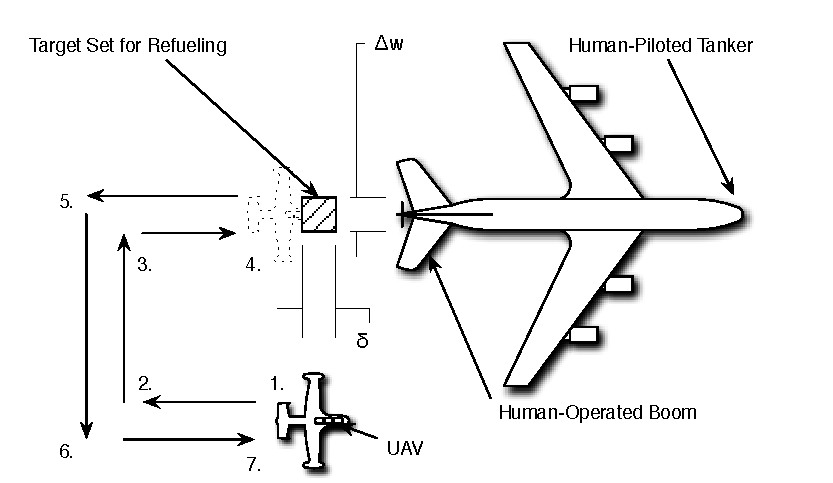
\includegraphics[width=0.7\textwidth]{img/overhead-crop}
	         \caption{Automted aerial refueling sequence.}
	         \label{fig:AAR_Diagram}
               \end{figure}

               Under a hybrid system abstraction, the discrete modes
               are the flight maneuvers performed in transitioning
               between the waypoints labeled in
               Figure~\ref{fig:AAR_Diagram}, while the continuous
               states are the relative coordinates of the tanker
               aircraft in the UAV reference frame, represented by a
               vector $x = (x_1, x_2, x_3)$ (the longitudinal,
               lateral, and heading coordinates, respectively). The
               relative motion between the tanker aircraft and UAV is
               then described by a kinematics model of the form
               $\dot{x}=f(x,u,d)$, where $u$ is the control input (in
               this case the translational and angular velocities of
               the UAV), and $d$ is the disturbance entering into the
               system (in this case the fluctuation in tanker velocity
               due to wind effects).

               The maneuver sequence design problem involves choosing
               the switching conditions between the flight maneuvers,
               as well as the continuous control laws for the input
               $u$, so as to ensure that a collision between UAV and
               tanker is prevented regardless of possible environment
               disturbances $d$ and command latencies.  Under our
               proposed approach, a reachability calculation is
               carried out for each flight maneuver in the refueling
               sequence to determine 1) the capture set, which is the
               set of aircraft states from which a target waypoint can
               be attained within a finite time horizon, and 2) the
               collision set, which is the set of aircraft states from
               which the trajectory of a flight maneuver passes
               through a collision zone centered on the tanker
               aircraft.  An example of these sets computed for the
               Precontact maneuver (transition between waypoints 2 and
               3) is shown in Figure~\ref{fig:reachset_Precontact}.

               \begin{figure}[thpb]
 	         \centering
	         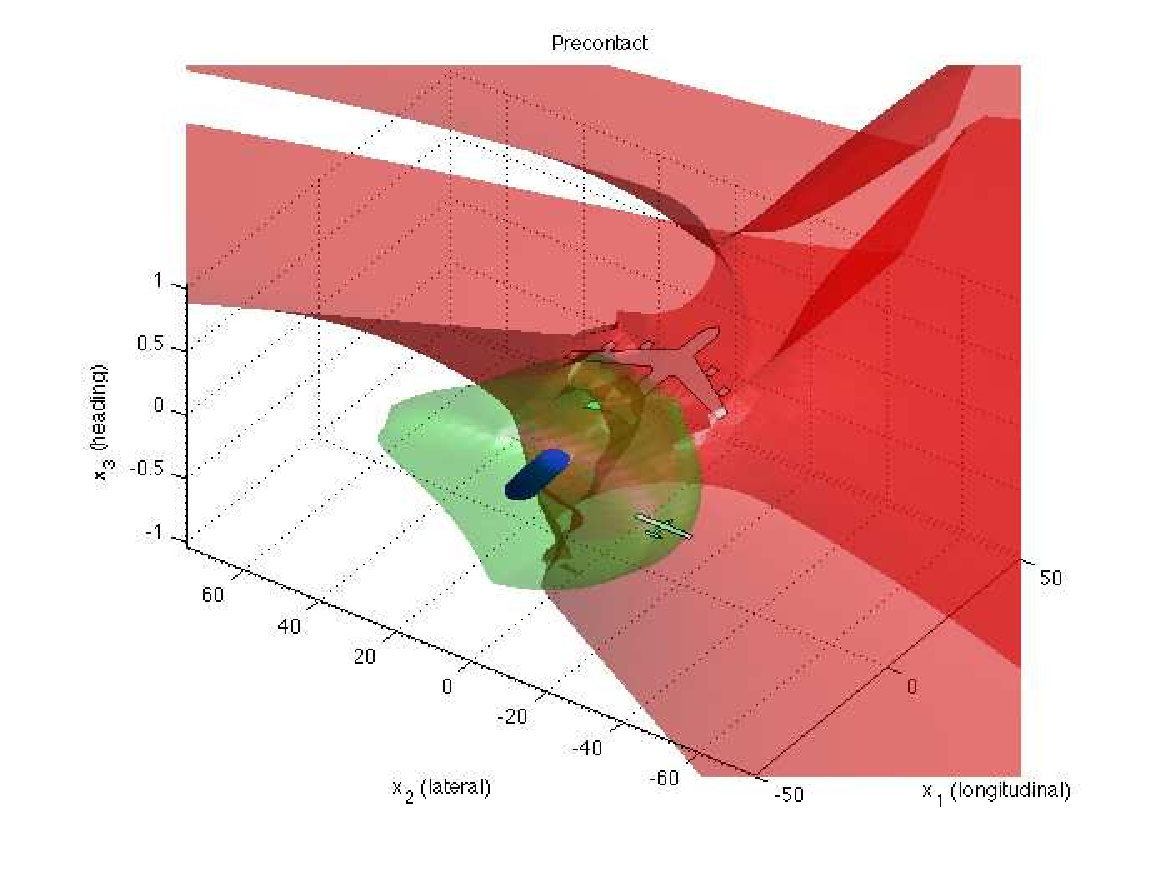
\includegraphics[width=0.7\textwidth]{img/reachset-precontact}
	         \caption{Capture set (light, green) and collision set (dark, red) computed for Precontact maneuver in aerial refueling sequence.}
	         \label{fig:reachset_Precontact}
               \end{figure}

               At design time, the capture sets and collision sets
               computed for the various maneuvers in the AAR sequence
               can be used to guide the choice of maneuver control
               laws and switching conditions to ensure that each
               maneuver terminates in an aircraft state that satisfies
               the target-attainability and safety objectives of the
               next maneuver (thus allowing the next maneuver to be
               feasibly initiated). Furthermore, through appropriate
               modifications of the reachability analysis, the effects
               of bounded disturbances and communication latency can
               also be taken into account. However, in such cases, the
               resulting design of maneuver control laws and switching
               conditions is in general more conservative than the
               case in which the robustness factors are not
               considered.  The performance of the control laws and
               switching conditions for the full AAR sequence has been
               validated in simulation with realistic model
               parameters, as detailed in \cite{j:ding-aiaa-gnd-2011}.


               \emph{b) Automatic Controller Synthesis for Switched Nonlinear Systems}

               While in certain applications a mode sequence is
               specified a priori according to designer insights,
               there are many cases in which one is simply given a set
               of controlled modes of operation and the task is to
               construct a mode selection policy, possibly as function
               of the state measurements, so as to ensure that desired
               control objectives are satisfied.  In particular,
               consider a switched nonlinear system of the following
               form:
               \begin{equation}
                 \label{eq:switched}
                 \dot{x}(t) = f_{q(t)}(x(t), u(t), d(t))
               \end{equation}
               where $\left\{f_q, q \in Q\right\}$ is a family of
               vector fields parametrized by a finite index set $Q$
               (for example a finite set of flight maneuvers); $u$ is
               a continuous control input; and $d$ is a disturbance
               input.

               We are interested in synthesizing controllers, which
               involves both a choice of the discrete mode $q$ and the
               continuous input $u$, so as to drive the continuous
               state $x$ into a set of goal configurations $R$, while
               avoiding an unsafe set $A$, subject to system dynamics
               (\ref{eq:switched}) and unknown but bounded,
               time-varying disturbances.  We call this a
               \textit{reach-avoid} problem.  For practical
               considerations, the controller is alllowed to modify
               input selections only at regularly spaced sampling
               instants, $t=0,T,...,NT$, at which measurements of the
               system state are received.

               In \cite{c:ding-CDC-2010} and \cite{c:ding-ICRA-2011},
               a solution to this controller synthesis problem is
               proposed, based upon iterative reachability
               calculations over sampling intervals.  In particular,
               we compute over successive iterations $k = 0,1,...,N$,
               the set of initial conditions $S_k$ for which there
               exists an admissible feedback policy satisfying the
               reach-avoid objectives over $[0,kT]$, subject to the
               worst-case disturbance, using a differential game
               formulation of reachability analysis.  The resulting
               set $S_N$ then provides us with the $N$-step feasible
               set for the reach-avoid problem.  Furthermore, as
               discussed in \cite{c:ding-CDC-2010}, we can derive from
               the representation of the sets $S_k$ a set-valued
               control law which satisfies the desired control
               objectives over $[0,kT]$.  By storing the reachable
               sets as lookup tables, one can then compute the
               appropriate control inputs in an online setting by
               checking set inclusions.  It has also been shown that a
               variant of this reachability calculation can be used to
               address the invariance problem, in which the objective
               is to remain within a desired set indefinitely
               \cite{c:ding-ICRA-2011}.

               We have applied this controller synthesis approach in
               an experimental setting to a target tracking problem,
               in which the objective is to control a quadrotor
               helicopter to first hover over a stationary ground
               vehicle and then track the vehicle as it starts moving,
               while satisfying certain velocity constraints.  In this
               case, the modes of the system are used to represent
               discrete choices of roll and pitch angles, which
               affects the quadrotor acceleration in the $x$ and $y$
               directions, while disturbances appear in the form of
               model uncertainties, as well as the movement of the
               ground vehicle, which is not planned ahead of time.

               Using the procedure described previously, we computed
               the set of initial conditions in the relative
               position-velocity space reachable to the hover region
               over 2.5 seconds, with the results shown in Figure
               \ref{fig:target_tracking}(a).  The control policy
               derived from this reachability computation was then
               implemented onboard the Stanford Testbed of Autonomous
               Rotorcraft for Multi-Agent Control (STARMAC).  The
               trajectories from an experimental run are shown in
               Figure \ref{fig:target_tracking}(b).  It can be seen
               that the quadrotor indeed enters the hover region
               within the time horizon of interest, and then remains
               within this region for the rest of the experiment,
               despite movements of the ground vehicle.
               \begin{figure}[thpb]
 	         \centering
	         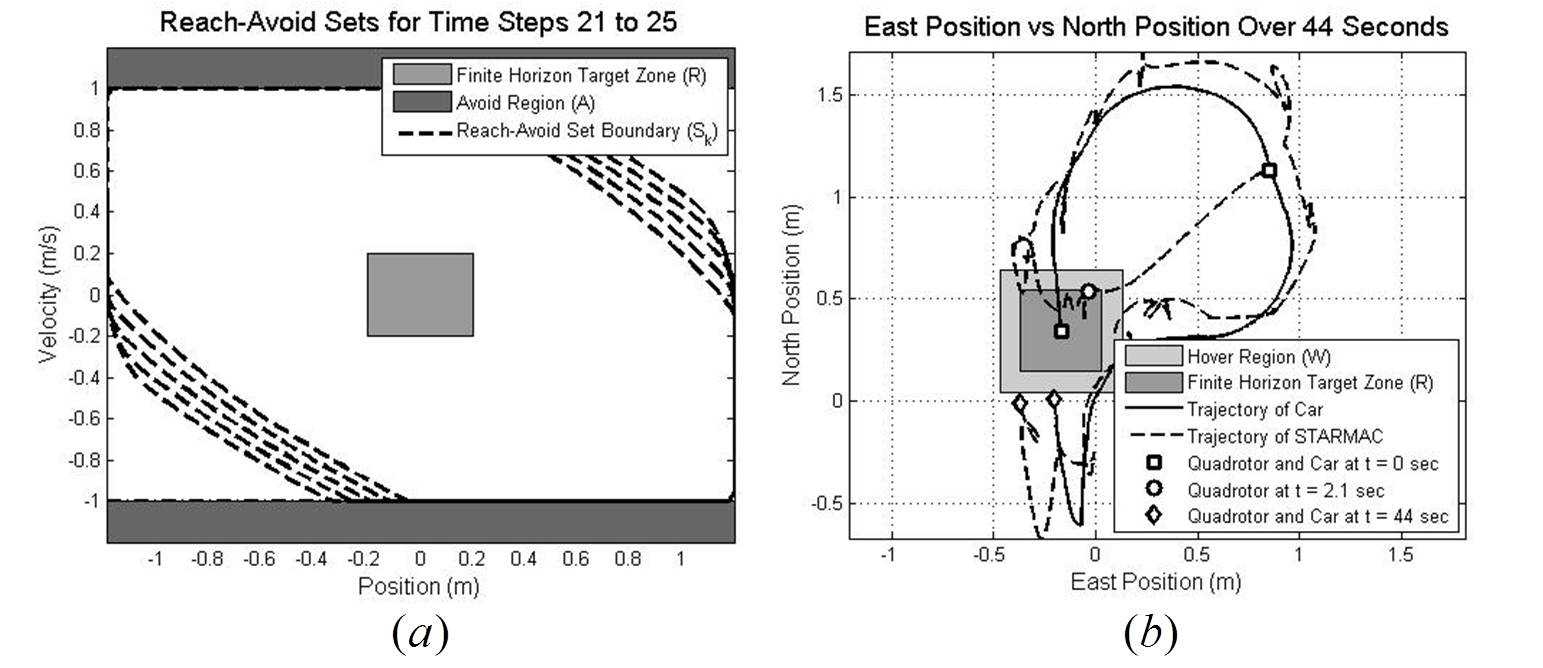
\includegraphics[width=0.9\textwidth]{img/target-tracking-plots}
	         \caption{Results for target tracking application: (a) reach-avoid sets in position-velocity space over 2.5 seconds ($T = 0.1$ s); (b) experimental trajectories of quadrotor and ground vehicle.}
	         \label{fig:target_tracking}
               \end{figure}



\subsubsection{Optimal Control of Switched Hybrid Dynamical Systems (Sastry, Tomlin)}

A natural extension of classical dynamical systems, where the state of the system is governed by a single differential equation, are switched dynamical systems, where the state of a system is governed by a finite number of differential equations, each of which can be arbitrarily chosen at an instant of time. The control parameter for such systems has a discrete component, the sequence of modes, and two continuous components, the duration of each mode and the continuous input. Switched systems arise in numerous modeling applications \cite{brockett1995stabilization, rantzer_switch}. 

Stemming from Branicky et al.'s seminal work that established a necessary condition for the optimal trajectory of switched systems in terms of quasi-variational inequalities \cite{branicky1998ufh}, there has been growing interest in the optimal control of such systems. However, Branicky provided only limited means for the computation of the required control. Others have employed variants of dynamic programming to develop algorithms to address the special case of piecewise-linear or affine systems \cite{bemporad2000piecewise,borrelli_hybrid,giua2001optimal}. Since after each iteration of these algorithms the number of possible switches grows exponentially, the representation of the optimal value function becomes increasingly complex. These approaches focus on addressing this particular shortcoming by considering a variety of possible relaxations of the optimal value function. 

Several address just the continuous component of the optimal control of an unconstrained nonlinear switched system while keeping the sequence of modes fixed. Given a fixed mode schedule, Xu et al. develop a bi-level hierarchical optimization algorithm:  at the higher level, a conventional optimal control algorithm finds the optimal continuous input assuming fixed mode duration and at the lower level, a conventional optimal control algorithm finds the optimal mode duration while keeping the continuous input fixed \cite{xu2003}. Axelsson et al. consider the special case of unconstrained nonlinear autonomous switched systems (i.e. systems wherein the control input is absent) and develop a similar bi-level hierarchical algorithm: at the higher level, the algorithm updates the mode sequence by employing a single mode insertion technique, and at the lower level, the algorithm assumes a fixed mode sequence and minimizes the cost functional over the switching times \cite{axelsson2008,egerstedt2006}. 

We generalized Axelsson's approach by constructing an optimal control algorithm for constrained nonlinear switched dynamical systems \cite{gonzalez2010descent, gonzalez2010cdc}. In our first paper we developed a bi-level hierarchical algorithm that divided the problem into two nonlinear constrained optimization problems. At the lower level, our algorithm assumed a fixed modal sequence and determined the optimal mode duration and optimal continuous input. At the higher level, our algorithm employed a single mode insertion technique to construct a new lower cost sequence. The result of our approach was an algorithm that provided a sufficient condition to guarantee the local optimality of the mode duration and continuous input while decreasing the overall cost via mode insertion. Though this was a powerful outcome given the generality of the problem under consideration, it suffered from three shortcomings which made its immediate application difficult. First, if our algorithm was initialized at an infeasible point it was unable to find a feasible lower cost trajectory. Unfortunately, initializing an optimization algorithm with a feasible point is nontrivial. Second, our algorithm did not incorporate multiple objectives into its cost function, which is useful for path planning type tasks. Finally, our algorithm did not penalize the number of hybrid jumps. In our second paper we design a new algorithm to address these three deficiencies and detail the utility of this modified approach on two examples.


We are interested in the optimal control of dynamical systems whose trajectory is governed by a differential equation of the form:
\begin{equation}
  \dot{x}(t) = f\big( x(t), u(t), d(t) \big), \quad \forall t\geq0,\quad x(0) = x_0,
\end{equation}
where $u: [0,\infty) \to \mathbb{R}^m$ is continuous input and $d: [0,\infty) \to \{ 1, 2, \ldots, Q \}$ is the discrete input. Instead of directly optimizing over the discrete input $d$, we optimize over the sequence $\sigma: \mathbb{N} \to \{ 1, 2, \ldots, Q \}$ and $s: \mathbb{N} \to [0,\infty)$, where it must be noted that given a pair $(\sigma,s)$ one can construct a discrete input recursively by, given $k \in \mathbb{N}$, applying the input $\sigma(k)$ for $s(k)$, and then repeat replacing $k$ with $k+1$. Also, since we want to account for several objectives as mentioned above, we introduce a extra variable $w: \{ 1, 2, \ldots, W \} \to \mathbb{N}$ which indexes the objectives.

Our algorithm finds a numerical solution of the following problem:
\begin{flalign}
  & {(OCP)} & 
  & \min_{ \sigma, s, u, w }\ \int_0^T L \big( x(t), u(t), t \big) dt + \sum_{k=1}^W \phi_k\big( x( \tau_{w(k)} ) \big) + C \#\sigma, & 
  & 
\end{flalign}
subject to:
\begin{align}
  & \tau_k = \sum_{i=1}^k s(i),\\
  & \dot{x}(t) = f\big( x(t), u(t), d(t) \big), \quad t \in [0,T], \quad x(0) = x_0,\\
  & \text{$d$ is constructed from the pair $(\sigma,s)$,}\\
  & h_j\big( x(t) \big) \leq 0, \quad \forall t \in [0,T], \quad j \in \{ 1, 2, \ldots, J \}.
\end{align}
The problem $(OCP)$ has both continuous as well as discrete variables, thus it is usually solved numerically using Integer Programming algorithms, which suffer the curse of dimensionality, i.e. as the size of the discrete variable increases linearly the number of function evaluations increases exponentially. Our algorithm offers numerical solutions which are not strict minimizers (i.e. our algorithm might stop at points that are not necessarily global minimizers) but it does not suffer the curse of dimensionality.

The algorithm solves a two-level optimization problem. In the first level it fixes $\sigma$ and $w$ and it minimizes $s$ and $u$ using known optimal control techniques as the ones in \cite{polak1997}. The second level performs a first-order variation of the cost function after the instantaneous insertion of an extra mode at a particular time: if the variation results in a decrease of the cost, then create a new sequence $\sigma$ including that insertion and repeat the process. This procedure converges to a class of points where the first-order variation produces no change in the cost, and hence no single mode insertion can further decrease the cost \cite{gonzalez2010descent, gonzalez2010cdc}.

As an example, we consider the optimal control of a quadrotor helicopter in 2D using a model described in \cite{gillula2011applications}. The evolution of the quadrotor can be defined with respect to a fixed 2D reference frame using six dimensions where the first three dimensions represent the position along a horizontal axis, the position along the vertical axis and the roll angle of the helicopter, respectively, and the last three dimensions represent the time derivative of the first three dimensions. We model the dynamics as a three mode switched system (the first mode describes the dynamics of going up, the second mode describes the dynamics of moving to the right, and the third mode describes the dynamics of moving to the left) with a single input as described in Table \ref{tab:ocp_dynamics} where $L = 0.305$ meters, $M = 1.3$ kilograms, $I = 0.0605$ kilogram meters squared and $g = 9.8$ meters per second squared. The cost and input constraints are as described in Table \ref{tab:ocp_cost} where the waypoints, $\hat{w}(i)$, are:
\begin{equation}
	\hat{w}(1) = 
  \begin{bmatrix} 
    2 \\ 5 \\ \pi 
  \end{bmatrix} 
  \ \text{and}\  
  \hat{w}(2) = 
  \begin{bmatrix} 
    4 \\ 1 \\ 0 
  \end{bmatrix},	
\end{equation}
and the time-varying desired trajectory is defined as:
\begin{equation}
	r(t) = 
	\begin{cases}
		(t,1), & \mbox{ if } t < 2 \\ 
		(2+\cos\left(t - 2 - \frac{\pi}{2}\right), 3+2\sin\left(t - 2 - \frac{\pi}{2}\right), & \mbox{ if } t < 2 + 2\pi \\
		(t-2+2\pi,1), & \mbox{ if } t < 4 + 2\pi \\
		(4,1), & \mbox{ else }
	\end{cases}
\end{equation}
The state is constrained to remain above the ground and outside of a box of height and width both equal to $1$ centered at $(1,1)$. The result of iterations $1$, $7$, and $10$ of the algorithm are shown in Figure \ref{fig:starmacexample}.


\begin{table}[t]
  \begin{center}
    \begin{tabular}{cc}
      Mode 1: & 
      $\ddot{x}(t) = \begin{bmatrix} \frac{\sin x_3(t)}{M}\left( u(t) + Mg \right) \\	\frac{\cos x_3(t)}{M}\left( u(t) + Mg \right) - g \\ 0 \\ \end{bmatrix}$ \\
      Mode 2: & 
      $\ddot{x}(t) = \begin{bmatrix} g\sin x_3(t) \\ g\cos x_3(t) - g \\ \frac{-L u(t)}{I} \\ \end{bmatrix}$ \\
      Mode 3: &
      $\ddot{x}(t) = \begin{bmatrix} g\sin x_3(t) \\	g\cos x_3(t) - g \\ \frac{L u(t)}{I} \\ \end{bmatrix}$ \\
    \end{tabular}
  \end{center}
  \caption{The dynamics of each of the modes of the quadrotor for our example.}
  \label{tab:ocp_dynamics} 
\end{table}

\begin{table}[t]
  \begin{center}
    \begin{align*}
      L(x(t),u(t),t) &= 10 \sum_{j=1}^2 \big(x_j(t) - r_j(t) \big)^2 \\
      \phi_k \big( x( \tau ) \big) &= 100 \sum_{j=i}^2 \big( x_j(\tau) - \hat{w}_j(i) \big)^2 + 1000 \left( \sin^2 \left( \frac{x_3(\tau) - \hat{w}_3(i)}{2} \right) \right) \\
      C &= 1
    \end{align*}
  \end{center}
  \caption{The components of the cost function, the input constraints, and the parameters of the optimality function for our example.}
  \label{tab:ocp_cost}
\end{table}


\begin{figure}[!t]
  \begin{minipage}{\columnwidth}
    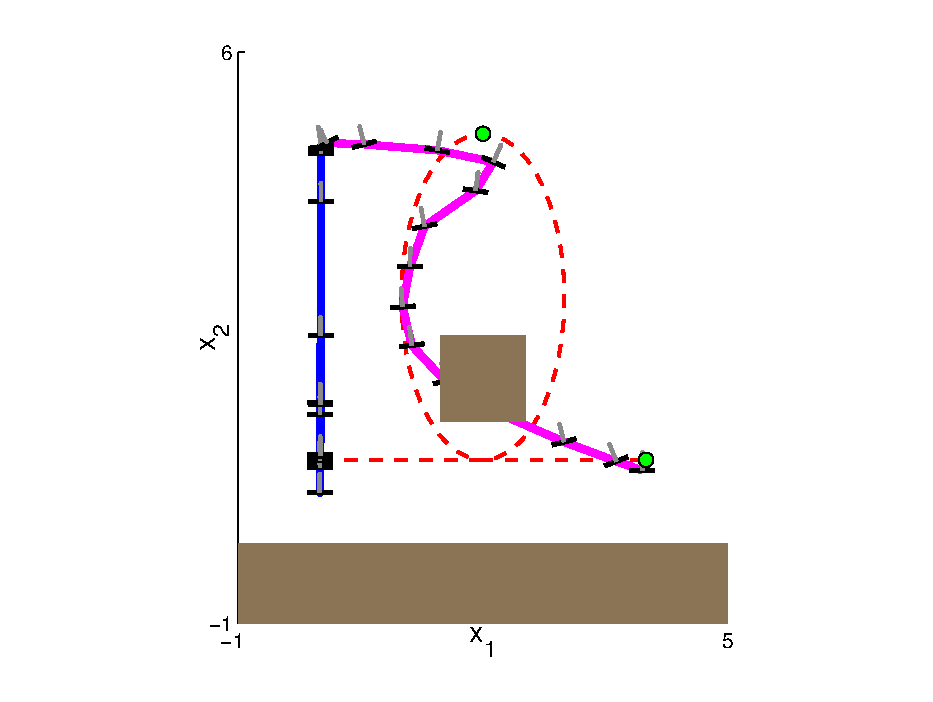
\includegraphics[clip, trim = 3.25cm .75cm 3.25cm .75cm, width = .32\columnwidth, keepaspectratio = true]{img/starmac_wp2_iter1}
    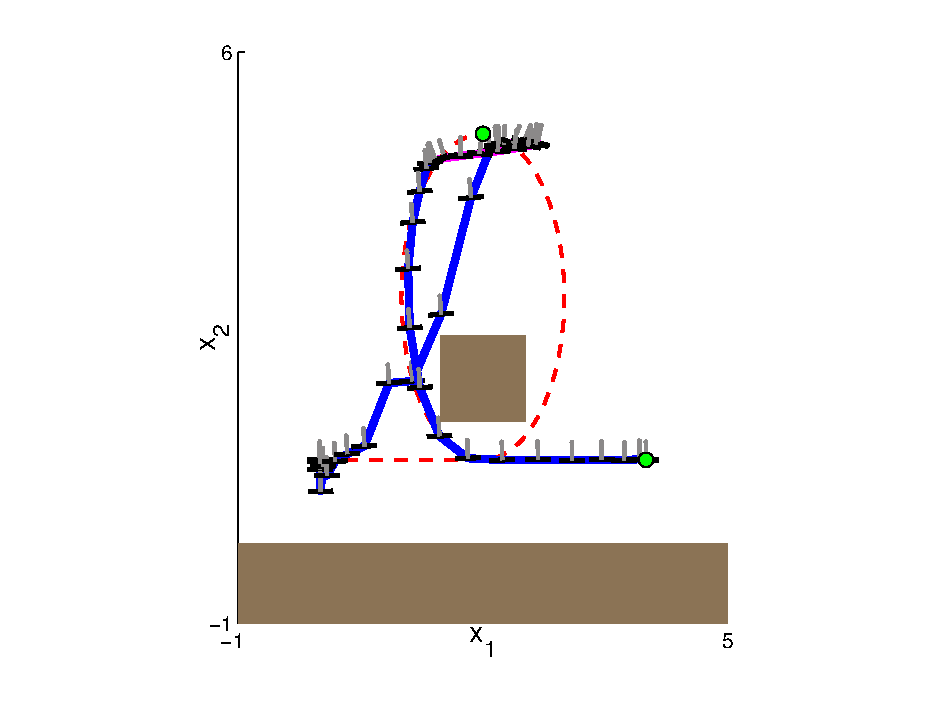
\includegraphics[clip, trim = 3.25cm .75cm 3.25cm .75cm, width = .32\columnwidth, keepaspectratio = true]{img/starmac_wp2_iter7}
    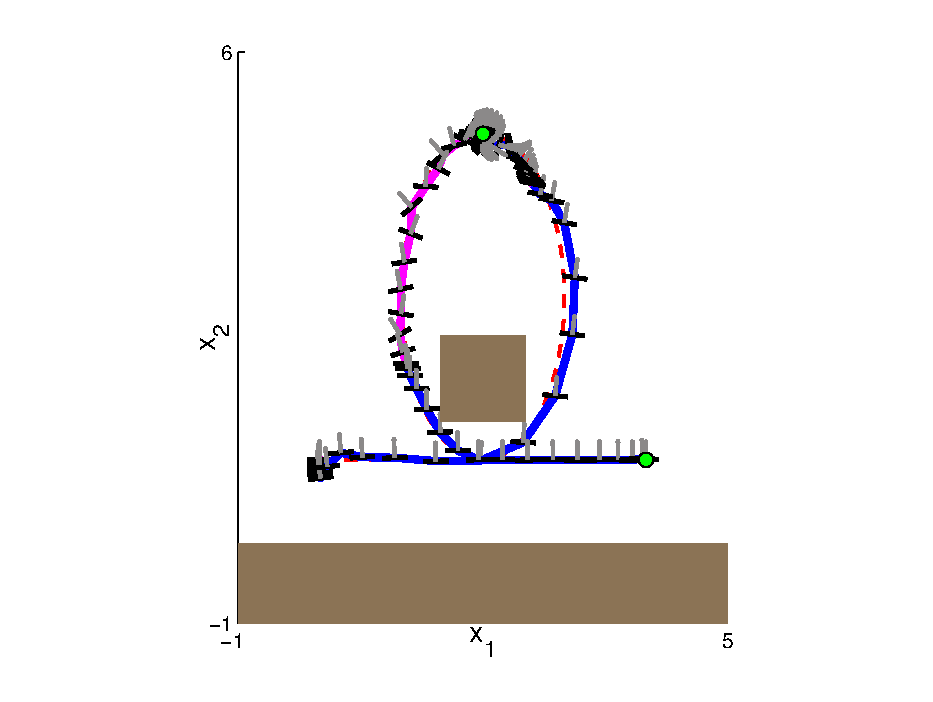
\includegraphics[clip, trim = 3.25cm .75cm 3.25cm .75cm, width = .32\columnwidth, keepaspectratio = true]{img/starmac_wp2_iter10}
  \end{minipage}
  \caption{Optimal trajectories (the quadrotor is drawn in black and the normal direction to the frame is drawn in gray) on the top row and bottom left in an environment with constraints (drawn in brown) and objectives (drawn in green). The first image shows iteration 1, the second iteration 7, and the third is iteration 10.}
  \label{fig:starmacexample}
\end{figure}


%%%%%%%%%%%%%%%%%
%%%%%%%%%%%%%%%%%
\subsubsection{Embedded Systems Modeling and Deep Compositionality (Krogh, Tomlin, Sastry)}
                 
                 \emph{Verification of Stochastic Hybrid Systems}
                 %    \newline \small{ Graduate Student: Maryam Kamgarpour}

                 \begin{figure}[!t]
                   \begin{center}
                     \begin{subfigmatrix}{2}% number of columns
                       \subfigure[Reach-Avoid problem]{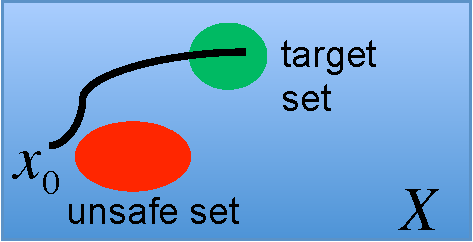
\includegraphics{img/reachavoidsets.pdf}}                
                       \subfigure[Probabilistic backward reach-avoid set]{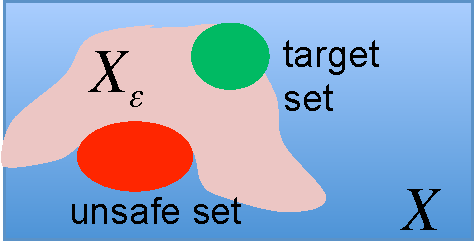
\includegraphics{img/reachavoidoptimal.pdf}}
                     \end{subfigmatrix}   
                     \caption{Reach-avoid problem for stochastic hybrid systems}
                     \label{fig:reach_avoid_problem}
                   \end{center}
                 \end{figure}

         

                 We consider a general hybrid modeling framework in
                 which we account for stochastic disturbances in
                 evolution of the continuous and discrete states. In
                 addition, we account for deterministic disturbances
                 in the model. The motivation is that while some
                 classes of uncertainty, such as those by nature, are
                 best modeled stochastically, some other classes of
                 uncertainty, such as those due to presence of agents
                 with competing objectives, are best modeled in a
                 deterministic worst-case approach. For example, in a
                 collision avoidance scenario between two aircraft, on
                 the one hand, wind affects the dynamics of aircraft
                 and uncertainties in wind forecast and measurement
                 may be best accounted for through a stochastic
                 framework. On the other hand, in the absence of
                 communication between the aircraft, from the
                 perspective of each aircraft, the trajectory must be
                 safe in the worst-case performance of the other
                 aircraft. Hence, a robust approach should be
                 considered.

                 The reach-avoid objective in the setting of the
                 stochastic hybrid system with two players becomes a
                 stochastic game in which the objective of player 1
                 (the control) is to steer the hybrid system state
                 into a desired target set, while avoiding a set of
                 unsafe states, as shown in Figure
                 \ref{fig:reach_avoid_problem}(a).  On the other hand,
                 the objective of player 2 (the adversary) is to
                 either steer the state into the unsafe set or prevent
                 it from reaching the target set.

                 Mathematically, the problem is stated as follows: Let
                 $X$ denote the hybrid state space. Suppose that Borel
                 sets $G, S \in \mathcal{B}(X)$ are given as the
                 desired target set and safe set, respectively, with
                 $G \subseteq S$.  Then the probability that the state
                 trajectory $(x_0, x_1, \dots, x_N)$ reaches $G$ while
                 staying inside $S$ under fixed choices of player 1
                 policy $\mu \in \mathcal{M}_a$ and player 2 strategy
                 $\gamma \in \Gamma_d$ is \cite{kamgar2011cdc}:

                 \begin{align*}
                   \label{eq:reachavoid_prob_expectation}
                   r_{x_0}^{\mu, \gamma}&(G,S) = E^{\mu,\gamma}_{x_0} \left[ \mathbf{1}_G(x_0) + \sum^{N}_{j=1}\left(\prod^{j-1}_{i=0}\mathbf{1}_{S\setminus G}(x_i)\right)\mathbf{1}_G(x_j)\right],
                 \end{align*}
                 where $E^{\mu,\gamma}_{x_0}$ denotes the expectation
                 with respect to the probability measure
                 $P_{x_0}^{\mu, \gamma}$ induced by the initial
                 condition, $x_0 \in X$, and the players'
                 strategies. The admissible control spaces consist of
                 the set of Markov policies and strategies, denoted by
                 $\mathcal{M}_a$, $\Gamma_d$, for the control and
                 adversary, respectively.

                 Define the worst-case reach-avoid probability under a
                 choice of Markov policy $\mu$ as $r_{x_0}^\mu(G,S) =
                 \inf_{\gamma \in \Gamma_d} r_{x_0}^{\mu,
                   \gamma}(G,S).$ Our objective is to maximize this
                 worst-case probability over the set of Markov
                 policies. Thus, we need to compute the maxmin value
                 function $r_{x_0}^*(G,S) := \sup_{\mu \in
                   \mathcal{M}_a} r_{x_0}^\mu(G,S)$, and find a maxmin
                 policy $\mu^* \in \mathcal{M}_a$, such that
                 $r_{x_0}^*(G,S) = r_{x_0}^{\mu^*}(G,S)$, $\forall x_0
                 \in X$.

                 We have developed a dynamic programming algorithm for
                 maximizing the reach-avoid probability and for
                 synthesizing a control law that achieves this
                 probability. In addition, from this algorithm we can
                 find the set of initial conditions $X_\epsilon$ for
                 which the reach-avoid probability is above
                 $(1-\epsilon)$, $\forall \epsilon \in [0,1]$, under
                 the worst-case adversary behavior, as shown in Figure
                 \ref{fig:reach_avoid_problem}(b).

                 The algorithm has been applied to several robust
                 motion planning problems including a quadrotor
                 helicopter tracking a ground vehicle and aircraft
                 conflict detection and resolution scenarios
                 \cite{kamgar2011cdc}.

                 \emph{Aircraft Conflict Detection}

                 The scenario involves two aircraft with possibly
                 intersecting nominal trajectories. From the
                 perspective of the first aircraft, the task is to
                 detect the possibility of conflict given current
                 position of another aircraft, and design a collision
                 avoidance trajectory in case potential conflict is
                 detected. Motivated by wind influence on aircraft
                 trajectories and on accuracy of conflict detection,
                 we consider wind with a deterministic component,
                 known through forecast or measurements, and a
                 stochastic component to capture its
                 uncertainties. Based on geostatistics analysis of
                 wind data, the stochastic wind component is modeled
                 as a time dependent random field over the $2D$
                 airspace.

                 A conflict is defined if aircraft get closer than a
                 critical distance of $R_c$. Hence, the safe set in
                 $2D$ can be defined in relative coordinates as: $S =
                 \{ (x^1,x^2) \in \mathbb{R}^2 \; s. t. \; \|
                 (x^1,x^2) \|_2 \geq R_c \}$.For conflict detection,
                 we assume that the current position of each aircraft
                 is available, for example through Automatic Dependent
                 Surveillance-Broadcast (ADS-B) network. For the
                 conflict resolution, we assume that the control of
                 the two aircraft are decentralized. Furthermore, in
                 the absence of further information on the decision
                 algorithms, each aircraft assumes that the other
                 aircraft could potentially make choices that endanger
                 safety.


                 The aircraft kinematics is modeled as a unicycle. The
                 input of each aircraft is its heading angle
                 rate. Motivated by discrete maneuvers used in air
                 traffic, we assume at any given time, each aircraft
                 can choose to be in one of three flight maneuvers:
                 straight, right turn, or left turn.

                 \begin{figure}[!t]
                   \begin{center}
                     \begin{subfigmatrix}{2}
                       \subfigure[Maxmin probability of safety]{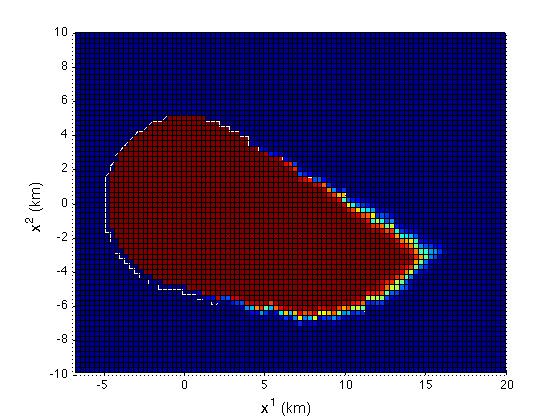
\includegraphics{img/pminmax_3pi4}}                
                       \subfigure[Deterministic reachable set]{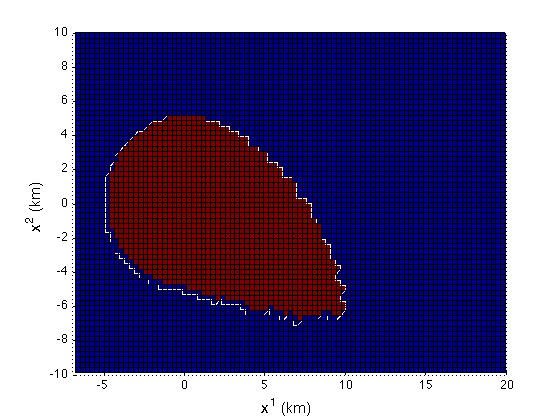
\includegraphics{img/deterministic_3pi4}}
                     \end{subfigmatrix}
                     \caption{Collision detection in probabilistic and deterministic settings}
                     \label{fig:prob_collision1}
                   \end{center}
                 \end{figure}

                 The maxmin probability of safety over a horizon of
                 $2.5$ minutes and with aircraft speed of $5$ km per
                 minute, is computed based on our proposed dynamic
                 programming algorithm. Figure
                 \ref{fig:prob_collision1}(a) illustrates this
                 probability for the set of initial conditions with
                 relative heading of $\frac{3\pi}{4}$ radians. The
                 interpretation of this probability map is as
                 follows. Consider an initial condition of $(10.55
                 \text{ km}, -6.85 \text{ km},\frac{3\pi}{4} \text{
                   rad})$. From the value function we obtain the
                 maxmin probability of safety to be $99 \%$.  This
                 means that if aircraft 1 selects flight maneuvers
                 according to the maxmin policy $\mu^*$ and aircraft 2
                 selects any maneuvers within the set of Markov
                 strategies, the probability of collision would remain
                 at most $1 \%$. For comparison, the result of
                 deterministic computation, in which wind influence is
                 ignored, is shown in Figure
                 \ref{fig:prob_collision1}(b). In this case, any
                 initial condition is characterized as being safe or
                 not.

                 \emph{Uncertain Safe and Target Sets}

                 \begin{figure}[!t]
                   \begin{center}
                     \begin{subfigmatrix}{2}
                       \subfigure[VIL measurements from forecast]{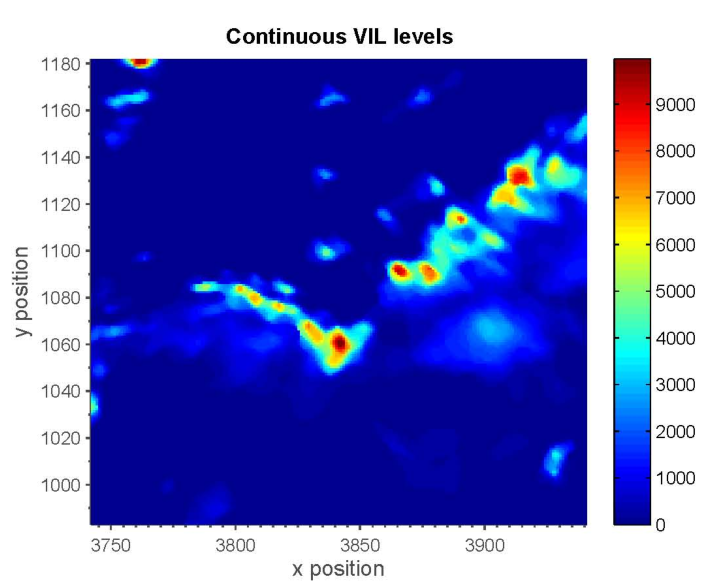
\includegraphics{img/VILcontinuous}}                
                       \subfigure[No-fly zones based on forecast]{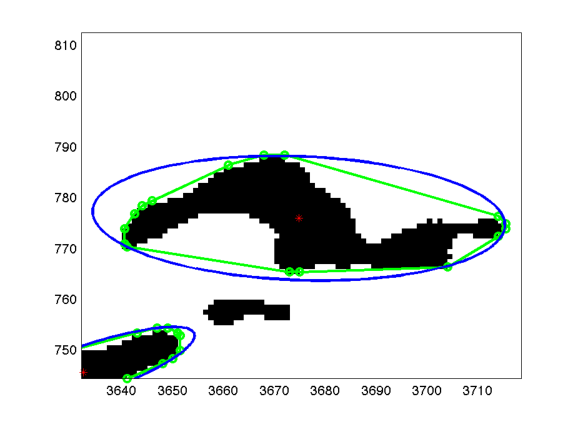
\includegraphics{img/VILenclosed}}
                     \end{subfigmatrix}
                     \caption{Forecast data for Vertically Integrated Liquid level}
                     \label{fig:vil}
                   \end{center}
                 \end{figure}

                 It has been shown that high values of Vertically
                 Integrated Liquid (VIL) level indicate storm
                 precipitation and regions with high VIL levels should
                 be avoided by pilots. We have used MIT Lincoln lab
                 forecast of VIL data over a gridded United States
                 airspace to characterize obstacles in aircraft
                 flight. Figure \ref{fig:vil}(a) shows the forecast
                 data for 01/07/2009 near gulf coast of Florida, while
                 Figure \ref{fig:vil}(b) shows the minimum-volume
                 geometric shapes enclosing the regions with high VIL
                 values in order to use them in an optimization
                 algorithm. In \cite{maryam2011ifac} we used a
                 deterministic hybrid optimal control approach to find
                 fuel efficient aircraft trajectories which avoid
                 these hazardous regions. Also, based on the actual
                 and forecast data, we modeled the storm movement over
                 time and formulated a receding horizon nonlinear
                 program to design conflict-free aircraft trajectories
                 which avoid moving storms
                 \cite{kamgarpour2010cdc}. Clearly, the actual weather
                 deviates from the forecast, specially, with
                 increasing forecast horizon. To account for such
                 environmental uncertainties, we introduced a
                 parametrized set-valued stochastic process model for
                 the stochastic target and safe sets in the
                 reach-avoid problem. In
                 \cite{summers2011stochasticset} we showed that the
                 verification and control synthesis for stochastic
                 hybrid systems with stochastic sets can be addressed
                 by an appropriate dynamic programming algorithm.

                 We used our methodology to optimize the probability
                 that the aircraft attains a rectangular region around
                 a waypoint shown in Figure
                 \ref{fig:prob_decoupled}(b), while avoiding the
                 stochastic unsafe sets, representing the storm
                 locations, over the $30$ minute horizon and to
                 synthesize an optimal Markov policy that achieves
                 this probability. The optimal value function, is
                 shown in Figure \ref{fig:prob_decoupled}(a) for all
                 initial positions $(x_0,y_0)$ in $2D$ with an initial
                 heading angle of $\psi_0 = -0.785$ radians. An
                 example execution of the process is shown in Figure
                 \ref{fig:prob_decoupled}(b).
                 \begin{figure}
                   \begin{center}
                     \begin{subfigmatrix}{2}
                       \subfigure[Probability map for $\psi_0 =-0.785$]{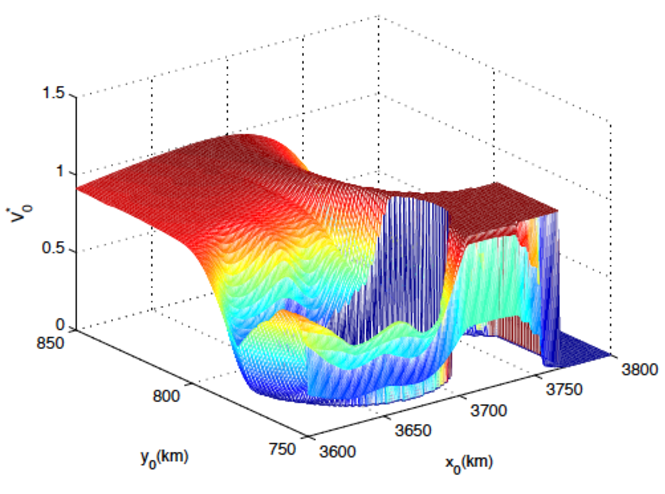
\includegraphics{img/Ch4ProbDecoupled}}                
                       \subfigure[Maximally safe trajectory]{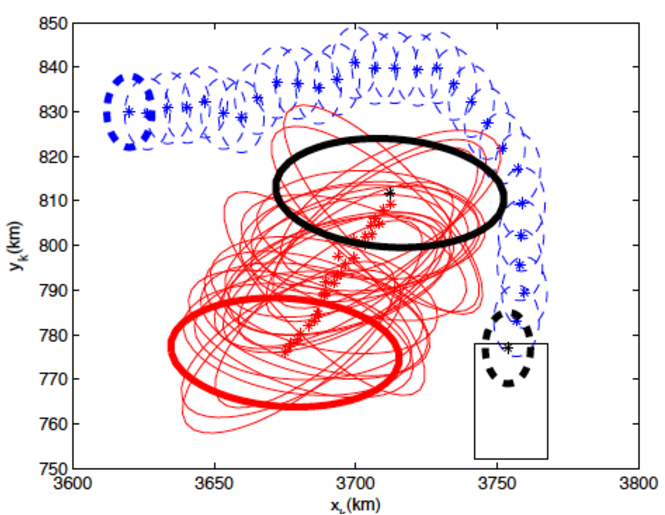
\includegraphics{img/Ch4PathDecoupled}}
                     \end{subfigmatrix}
                     \caption{Aircraft trajectory planning in stochastic environment}
                     \label{fig:prob_decoupled}
                   \end{center}
                 \end{figure}




               \subsubsection{Finite State Machines and Modal Models in Ptolemy II (Lee)}


               FSMs are actors whose behavior is described using a
               finite set of states and transitions between the
               states. The transitions between the states are enabled
               by guards, which are boolean-valued expressions that
               can reference inputs to the actor and parameters in
               scope. The transitions can produce outputs and can
               update the value of parameters in scope. Modal models
               extend FSMs by allowing states to have refinements,
               which are hierarchical Ptolemy II models. The
               refinements may themselves be FSMs, modal models, or
               any composite actor containing a director compatible
               with the domain in which the modal model is being
               used. On the basis of several examples, the memorandum
               describes the operational semantics, the practical
               usage, and the semantics of time in modal models.

               During this period, we released our update to the modal model system
               as part of Ptolemy II 8.0.1.  In addition we wrote a conference
               paper ``Modal Models in Ptolemy,''
               for the   Workshop on  Equation-Based Object-Oriented Modeling Languages and Tools,
               held in conjunction with MODELS
               \cite{LeeTripakis10_ModalModelsInPtolemyProceedings}
               \cite{LeeTripakis10_ModalModelsInPtolemyPresentation}, the
               abstract of which is reproduced below:
               \begin{quotation}
                 ``Ptolemy is an open-source and extensible modeling and simulation
                 framework. It offers heterogeneous modeling capabilities by allowing
                 different models of computation to be composed hierarchically in an
                 arbitrary fashion. This paper describes modal models, which allow to
                 hierarchically compose finite-state machines with other models of
                 computation, both untimed and timed. The semantics of modal models
                 in Ptolemy are defined in a modular manner.''
               \end{quotation}
               Model models were also covered in a
               general Ptolemy tutorial\cite{BrooksLeeTripakis10_ExploringModelsOfComputationWithPtolemyII}
               given at ESWeek 2010.



 

 \subsubsection{Verification of Hybrid Systems via Differential Invariants (Clarke, Platzer)}

Andr{\'e} Platzer has written a book about hybrid systems verification that will appear with Springer as "Logical Analysis of Hybrid Systems: Proving Theorems for Complex Dynamics." This book describes basic and advanced verification techniques for hybrid systems, including applications to air traffic control analysis. It will be a good introduction for graduate students working in the area.


\subsubsection{Embedded Convex Optimization (Boyd) }

This work concerns the use of convex optimization in high speed, real-time embedded systems, such as those found for signal processing, automatic control, estimation, resource allocation and decision making. While convex optimization is widely used on time scales of seconds or minutes, typically with a skilled engineer 'in the loop' supervising the optimization solver, it is less commonly seen for real-time applications.

A primary concern in real-time or embedded applications is the solver speed. We have ad-dressed this for a variety of applications, including using hand-coded solvers, including software for high-speed model predictive control (MPC).  Taking this work further, we have created an automatic code generator, CVXGEN, which takes a high-level description of a convex optimiza-tion problem and automatically generates compilable, library-free C code for a high speed solver.

This enables extensive (automatic) customization for the problem at hand, and makes solution much faster than existing methods. While with a hand-written solver, even small changes in problem specification necessitated painstaking redesign, even a complete change only requires the use of CVXGEN to automatically generate new code. This, combined with extremely fast solvers that carry out convex optimization on millisecond or even microsecond time scales, means that many new applications are possible, particularly for embedded systems.

A parallel branch of work investigates high-speed control algorithms for use in linear stochastic control. Here we evaluate a control-Lyapunov policy at each time step. For small problems the associated QP can be solved explicitly, but for larger problems on-line optimization is re-quired. This means the control-Lyapunov policy is often considered excessively computationally intensive for real-time or embedded systems. We have demonstrated several techniques for accelerating evaluation of control-Lyapunov policies, including the pre-computation of certain quantities, and the use of performance bounds that enable much faster approximate policies to be used instead. The performance bounds are computed offline using linear matrix inequalities and semidefinite programming.

Another related area of investigation has been algorithms for distributed optimization. Distributed optimization allows us to divide up computation of more complicated problems across multiple processing cores for faster computation. We have studied methods such as Alternating Directions Method of Multipliers, which provide a framework for decomposing convex optimization problems. Each subproblem can be solved completely in parallel, and the cores only need to communicate very simple messages during processing. With ever growing size and complexity of databases and information, using distributed optimization is increasingly becoming important to a wide range of problems in control, machine learning, portfolio optimization, network flow and scheduling. This will allow many of these problems (that have traditionally been considered slow) to be solved very fast and in real-time. 



%\subsubsection{Embedded Systems Modeling and Deep Compositionality (Krogh, Tomlin, Sastry)}
                 
                 \emph{Verification of Stochastic Hybrid Systems}
                 %    \newline \small{ Graduate Student: Maryam Kamgarpour}

                 \begin{figure}[!t]
                   \begin{center}
                     \begin{subfigmatrix}{2}% number of columns
                       \subfigure[Reach-Avoid problem]{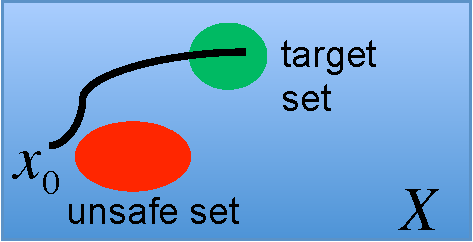
\includegraphics{img/reachavoidsets.pdf}}                
                       \subfigure[Probabilistic backward reach-avoid set]{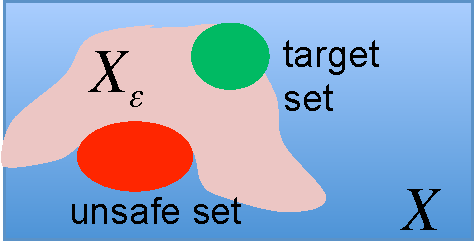
\includegraphics{img/reachavoidoptimal.pdf}}
                     \end{subfigmatrix}   
                     \caption{Reach-avoid problem for stochastic hybrid systems}
                     \label{fig:reach_avoid_problem}
                   \end{center}
                 \end{figure}

         

                 We consider a general hybrid modeling framework in
                 which we account for stochastic disturbances in
                 evolution of the continuous and discrete states. In
                 addition, we account for deterministic disturbances
                 in the model. The motivation is that while some
                 classes of uncertainty, such as those by nature, are
                 best modeled stochastically, some other classes of
                 uncertainty, such as those due to presence of agents
                 with competing objectives, are best modeled in a
                 deterministic worst-case approach. For example, in a
                 collision avoidance scenario between two aircraft, on
                 the one hand, wind affects the dynamics of aircraft
                 and uncertainties in wind forecast and measurement
                 may be best accounted for through a stochastic
                 framework. On the other hand, in the absence of
                 communication between the aircraft, from the
                 perspective of each aircraft, the trajectory must be
                 safe in the worst-case performance of the other
                 aircraft. Hence, a robust approach should be
                 considered.

                 The reach-avoid objective in the setting of the
                 stochastic hybrid system with two players becomes a
                 stochastic game in which the objective of player 1
                 (the control) is to steer the hybrid system state
                 into a desired target set, while avoiding a set of
                 unsafe states, as shown in Figure
                 \ref{fig:reach_avoid_problem}(a).  On the other hand,
                 the objective of player 2 (the adversary) is to
                 either steer the state into the unsafe set or prevent
                 it from reaching the target set.

                 Mathematically, the problem is stated as follows: Let
                 $X$ denote the hybrid state space. Suppose that Borel
                 sets $G, S \in \mathcal{B}(X)$ are given as the
                 desired target set and safe set, respectively, with
                 $G \subseteq S$.  Then the probability that the state
                 trajectory $(x_0, x_1, \dots, x_N)$ reaches $G$ while
                 staying inside $S$ under fixed choices of player 1
                 policy $\mu \in \mathcal{M}_a$ and player 2 strategy
                 $\gamma \in \Gamma_d$ is \cite{kamgar2011cdc}:

                 \begin{align*}
                   \label{eq:reachavoid_prob_expectation}
                   r_{x_0}^{\mu, \gamma}&(G,S) = E^{\mu,\gamma}_{x_0} \left[ \mathbf{1}_G(x_0) + \sum^{N}_{j=1}\left(\prod^{j-1}_{i=0}\mathbf{1}_{S\setminus G}(x_i)\right)\mathbf{1}_G(x_j)\right],
                 \end{align*}
                 where $E^{\mu,\gamma}_{x_0}$ denotes the expectation
                 with respect to the probability measure
                 $P_{x_0}^{\mu, \gamma}$ induced by the initial
                 condition, $x_0 \in X$, and the players'
                 strategies. The admissible control spaces consist of
                 the set of Markov policies and strategies, denoted by
                 $\mathcal{M}_a$, $\Gamma_d$, for the control and
                 adversary, respectively.

                 Define the worst-case reach-avoid probability under a
                 choice of Markov policy $\mu$ as $r_{x_0}^\mu(G,S) =
                 \inf_{\gamma \in \Gamma_d} r_{x_0}^{\mu,
                   \gamma}(G,S).$ Our objective is to maximize this
                 worst-case probability over the set of Markov
                 policies. Thus, we need to compute the maxmin value
                 function $r_{x_0}^*(G,S) := \sup_{\mu \in
                   \mathcal{M}_a} r_{x_0}^\mu(G,S)$, and find a maxmin
                 policy $\mu^* \in \mathcal{M}_a$, such that
                 $r_{x_0}^*(G,S) = r_{x_0}^{\mu^*}(G,S)$, $\forall x_0
                 \in X$.

                 We have developed a dynamic programming algorithm for
                 maximizing the reach-avoid probability and for
                 synthesizing a control law that achieves this
                 probability. In addition, from this algorithm we can
                 find the set of initial conditions $X_\epsilon$ for
                 which the reach-avoid probability is above
                 $(1-\epsilon)$, $\forall \epsilon \in [0,1]$, under
                 the worst-case adversary behavior, as shown in Figure
                 \ref{fig:reach_avoid_problem}(b).

                 The algorithm has been applied to several robust
                 motion planning problems including a quadrotor
                 helicopter tracking a ground vehicle and aircraft
                 conflict detection and resolution scenarios
                 \cite{kamgar2011cdc}.

                 \emph{Aircraft Conflict Detection}

                 The scenario involves two aircraft with possibly
                 intersecting nominal trajectories. From the
                 perspective of the first aircraft, the task is to
                 detect the possibility of conflict given current
                 position of another aircraft, and design a collision
                 avoidance trajectory in case potential conflict is
                 detected. Motivated by wind influence on aircraft
                 trajectories and on accuracy of conflict detection,
                 we consider wind with a deterministic component,
                 known through forecast or measurements, and a
                 stochastic component to capture its
                 uncertainties. Based on geostatistics analysis of
                 wind data, the stochastic wind component is modeled
                 as a time dependent random field over the $2D$
                 airspace.

                 A conflict is defined if aircraft get closer than a
                 critical distance of $R_c$. Hence, the safe set in
                 $2D$ can be defined in relative coordinates as: $S =
                 \{ (x^1,x^2) \in \mathbb{R}^2 \; s. t. \; \|
                 (x^1,x^2) \|_2 \geq R_c \}$.For conflict detection,
                 we assume that the current position of each aircraft
                 is available, for example through Automatic Dependent
                 Surveillance-Broadcast (ADS-B) network. For the
                 conflict resolution, we assume that the control of
                 the two aircraft are decentralized. Furthermore, in
                 the absence of further information on the decision
                 algorithms, each aircraft assumes that the other
                 aircraft could potentially make choices that endanger
                 safety.


                 The aircraft kinematics is modeled as a unicycle. The
                 input of each aircraft is its heading angle
                 rate. Motivated by discrete maneuvers used in air
                 traffic, we assume at any given time, each aircraft
                 can choose to be in one of three flight maneuvers:
                 straight, right turn, or left turn.

                 \begin{figure}[!t]
                   \begin{center}
                     \begin{subfigmatrix}{2}
                       \subfigure[Maxmin probability of safety]{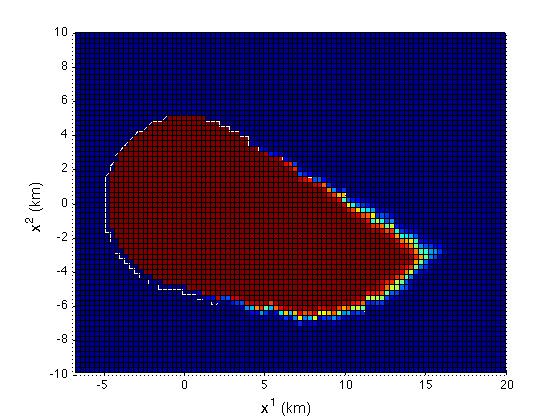
\includegraphics{img/pminmax_3pi4}}                
                       \subfigure[Deterministic reachable set]{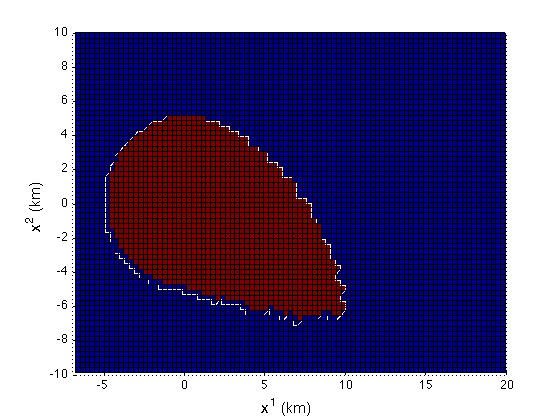
\includegraphics{img/deterministic_3pi4}}
                     \end{subfigmatrix}
                     \caption{Collision detection in probabilistic and deterministic settings}
                     \label{fig:prob_collision1}
                   \end{center}
                 \end{figure}

                 The maxmin probability of safety over a horizon of
                 $2.5$ minutes and with aircraft speed of $5$ km per
                 minute, is computed based on our proposed dynamic
                 programming algorithm. Figure
                 \ref{fig:prob_collision1}(a) illustrates this
                 probability for the set of initial conditions with
                 relative heading of $\frac{3\pi}{4}$ radians. The
                 interpretation of this probability map is as
                 follows. Consider an initial condition of $(10.55
                 \text{ km}, -6.85 \text{ km},\frac{3\pi}{4} \text{
                   rad})$. From the value function we obtain the
                 maxmin probability of safety to be $99 \%$.  This
                 means that if aircraft 1 selects flight maneuvers
                 according to the maxmin policy $\mu^*$ and aircraft 2
                 selects any maneuvers within the set of Markov
                 strategies, the probability of collision would remain
                 at most $1 \%$. For comparison, the result of
                 deterministic computation, in which wind influence is
                 ignored, is shown in Figure
                 \ref{fig:prob_collision1}(b). In this case, any
                 initial condition is characterized as being safe or
                 not.

                 \emph{Uncertain Safe and Target Sets}

                 \begin{figure}[!t]
                   \begin{center}
                     \begin{subfigmatrix}{2}
                       \subfigure[VIL measurements from forecast]{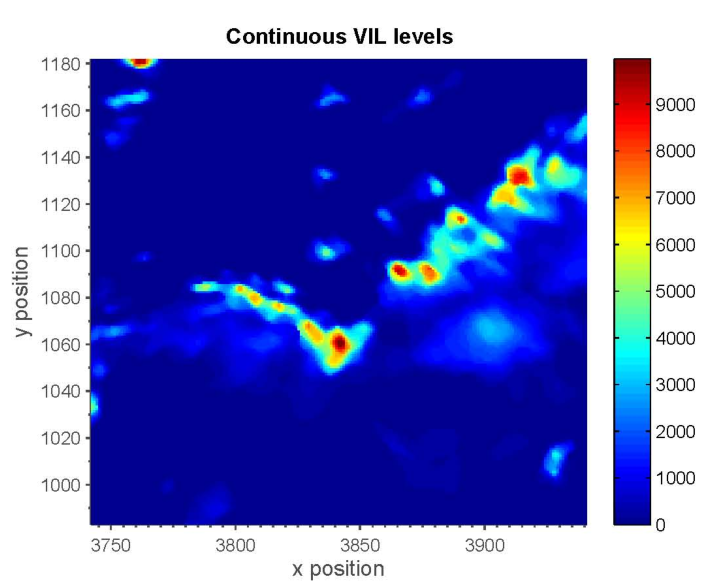
\includegraphics{img/VILcontinuous}}                
                       \subfigure[No-fly zones based on forecast]{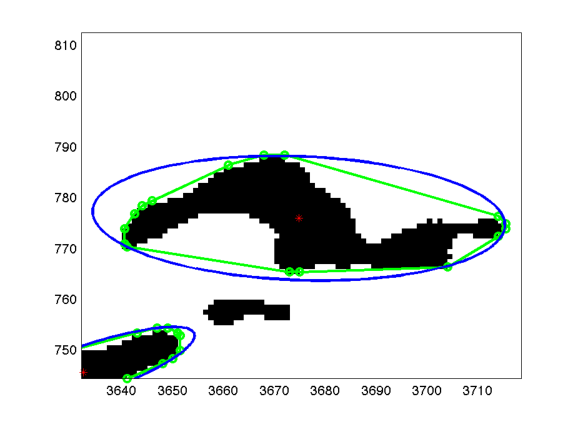
\includegraphics{img/VILenclosed}}
                     \end{subfigmatrix}
                     \caption{Forecast data for Vertically Integrated Liquid level}
                     \label{fig:vil}
                   \end{center}
                 \end{figure}

                 It has been shown that high values of Vertically
                 Integrated Liquid (VIL) level indicate storm
                 precipitation and regions with high VIL levels should
                 be avoided by pilots. We have used MIT Lincoln lab
                 forecast of VIL data over a gridded United States
                 airspace to characterize obstacles in aircraft
                 flight. Figure \ref{fig:vil}(a) shows the forecast
                 data for 01/07/2009 near gulf coast of Florida, while
                 Figure \ref{fig:vil}(b) shows the minimum-volume
                 geometric shapes enclosing the regions with high VIL
                 values in order to use them in an optimization
                 algorithm. In \cite{maryam2011ifac} we used a
                 deterministic hybrid optimal control approach to find
                 fuel efficient aircraft trajectories which avoid
                 these hazardous regions. Also, based on the actual
                 and forecast data, we modeled the storm movement over
                 time and formulated a receding horizon nonlinear
                 program to design conflict-free aircraft trajectories
                 which avoid moving storms
                 \cite{kamgarpour2010cdc}. Clearly, the actual weather
                 deviates from the forecast, specially, with
                 increasing forecast horizon. To account for such
                 environmental uncertainties, we introduced a
                 parametrized set-valued stochastic process model for
                 the stochastic target and safe sets in the
                 reach-avoid problem. In
                 \cite{summers2011stochasticset} we showed that the
                 verification and control synthesis for stochastic
                 hybrid systems with stochastic sets can be addressed
                 by an appropriate dynamic programming algorithm.

                 We used our methodology to optimize the probability
                 that the aircraft attains a rectangular region around
                 a waypoint shown in Figure
                 \ref{fig:prob_decoupled}(b), while avoiding the
                 stochastic unsafe sets, representing the storm
                 locations, over the $30$ minute horizon and to
                 synthesize an optimal Markov policy that achieves
                 this probability. The optimal value function, is
                 shown in Figure \ref{fig:prob_decoupled}(a) for all
                 initial positions $(x_0,y_0)$ in $2D$ with an initial
                 heading angle of $\psi_0 = -0.785$ radians. An
                 example execution of the process is shown in Figure
                 \ref{fig:prob_decoupled}(b).
                 \begin{figure}
                   \begin{center}
                     \begin{subfigmatrix}{2}
                       \subfigure[Probability map for $\psi_0 =-0.785$]{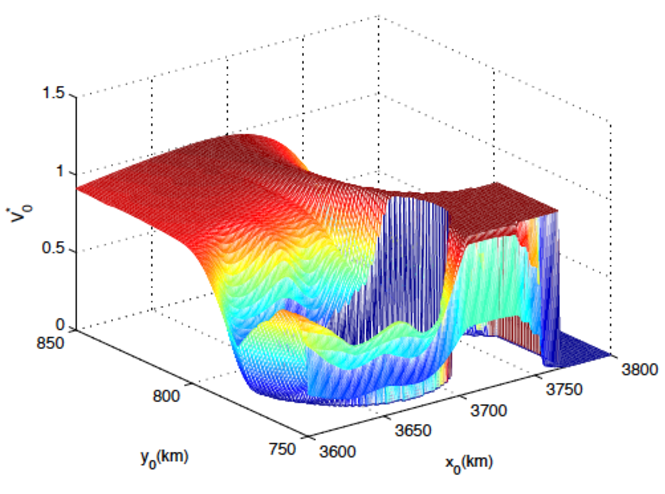
\includegraphics{img/Ch4ProbDecoupled}}                
                       \subfigure[Maximally safe trajectory]{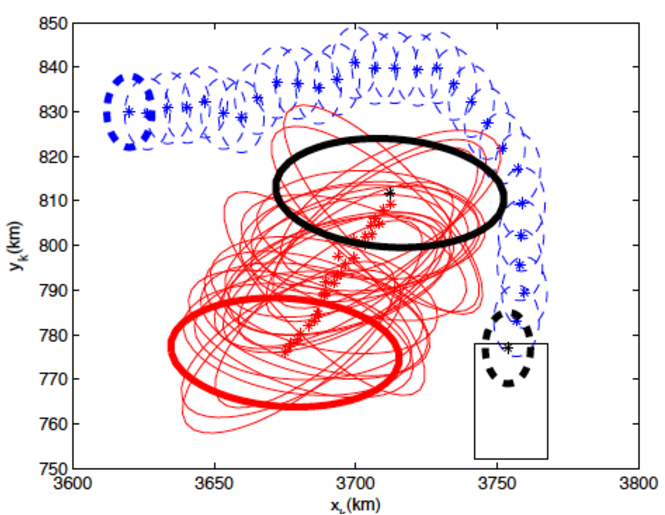
\includegraphics{img/Ch4PathDecoupled}}
                     \end{subfigmatrix}
                     \caption{Aircraft trajectory planning in stochastic environment}
                     \label{fig:prob_decoupled}
                   \end{center}
                 \end{figure}



\subsection{Model-Based Software Design and Verification}

\subsubsection{Advances in Verification and Reachability Analysis}

Reachability computations are foundational to the verification of continuous and hybrid dynamic systems.  In this MURI we made several advances in the development of reachability analysis techniques for continuous and hybrid dynamic systems.  We extended the concept of counterexample guided abstraction refinement (CEGAR) techniques in the verification of discrete systems to hybrid systems.  In a new method called iterative relaxation analysis, multiple abstractions are constructed such that the composition of the results for the collection of abstractions leads to a successful verification of the overall system.  This approach out-performs state-of-the-art reachability engines by a factor of 1000 on some examples.

We also developed reachability-based methods for verifying properties of numerical software, taking into account floating point errors.  The technique uses a new widening operator, similar to the types of operators used to guarantee convergence to a fixed point in abstract interpretation.  We developed a new bounded-time verification technique that combines software model checking and simulation.  The technique directly analyzes controller code and reachable set estimation via bisimulation functions is used to conservatively capture the behaviors of a plant with continuous dynamics.  We have also developed a new method for finding counterexamples that uses a software model checker to perform a systematic simulation of the software implementation of a controller coupled with a continuous plant. 

 In year 5 we developed new methods for computing tight overapproximations of reachable sets for linear dynamic systems with uncertain, time-varying parameters and bounded input signals.   This makes it possible to compute much tighter approximations to reachable sets for nonlinear systems using on-the-fly local linearizations.  Using zonotopes as the fundamental representation of sets, reachable sets can be computed for systems with dozens of continuous state variables.  Improvements of two to three orders of magnitudes in computation times have been achieved.

\subsubsection{Model-Integrated Computing (Sztipanovits, Karsai, Kottenstette, Hemingway, Porter)}

\emph{Cross-layer abstractions}

Model-based software design progresses along abstraction layers
(design platforms) capturing essential design concerns. Effectiveness of the model-based design
largely depends on how much the design concerns (captured in the abstraction layers) are orthogonal,
i.e., how much the design decisions in the different layers are independent. Heterogeneity
of embedded systems causes major difficulties in this regard. The controller dynamics is typically
designed without considering implementation side effects (e.g. numeric accuracy of computational
components, timing accuracy caused by shared resource and schedulers, time varying delays
caused by network effects, etc.). Compositionality in one layer depends on a web of assumptions
to be satisfied by other layers.

We have continued investigating theories and techniques for applying cross-layer abstraction
to make the controller designs robust against implementation side effects. We pursue this by inserting
implementation related abstractions in the controller design, and physical abstractions in
software design. The ultimate goal is decreasing the entanglement across the design layers.
We have developed model transformation tools that generate TrueTime abstractions from system
level models and investigate now the application of orthogonal structures in implementing
dynamics.


              \subsubsection{Autocoding Embedded Software for Safety Critical Systems (Lee)} 


               \emph{Code Generation}
               
               During this period, we enhanced the code generator so
               that we can generate code that calls user-defined actors
               for which we do not have code generation templates.  This
               feature allows the same user-generated code to be used in
               development and in deployment.

               In addition, we modified the code generator so that it can handle very
               large models and generate code that can be successfully compiled.  Our
               test case is a propietary model consisting of 19000 actors.  Our code
               generated created a 96Mb Java file that we were able to compile by
               implementing a number of tricks such as inner classes, static imports
               and using arrays instead of individual variables.  This work was done
               as part of the Extensible Modeling and Analysis Framework (EMAF) for
               AFRL.


               During this period we explored the theoretical
               ramifications of interface theory.  This work is
               critical if we are to be able to prove that that the
               clustering of models is correct.  Marc Geilen, visiting
               Berkeley from Eindhoven University of Technology,
               coauthored a paper with Stavros Tripakis (Berkeley) and
               Maarten Wiggers (Berkeley), ``The Earlier the Better: A
               Theory of Timed Actor Interfaces''
               \cite{GeilenTripakisWiggers11_EarlierBetterTheoryOfTimedActorInterfaces}

               \begin{quotation}
                 ``In a component-based design context, we propose a
                 relational interface theory for synchronous systems. A
                 component is abstracted by its interface, which
                 consists of input and output variables, as well as one
                 or more contracts. A contract is a relation between
                 input and output assignments. In the stateless case,
                 there is a single contract that holds at every
                 synchronous round. In the general, stateful, case, the
                 contract may depend on the state, modeled as the
                 history of past observations. Interfaces can be
                 composed by connection or feedback. Parallel
                 composition is a special case of connection. Feedback
                 is allowed only for Moore interfaces, where the
                 contract does not depend on the current values of the
                 input variables that are connected (although it may
                 depend on past values of such variables). The theory
                 includes explicit notions of environments, pluggability
                 and substitutability. Environments are themselves
                 interfaces. Pluggability means that the closed-loop
                 system formed by an interface and an environment is
                 well-formed, that is, a state with unsatisfiable
                 contract is unreachable. Substitutability means that an
                 interface can replace another interface in any
                 environment. A refinement relation between interfaces
                 is proposed, that has two main properties: first, it is
                 preserved by composition; second, it is equivalent to
                 substitutability for well-formed interfaces. Shared
                 refinement and abstraction operators, corresponding to
                 greatest lower and least upper bounds with respect to
                 refinement, are also defined. Input-complete
                 interfaces, that impose no restrictions on inputs, and
                 deterministic interfaces, that produce a unique output
                 for any legal input, are discussed as special cases,
                 and an interesting duality between the two classes is
                 exposed. A number of illustrative examples are
                 provided, as well as algorithms to compute
                 compositions, check refinement, and so on, for
                 finite-state interfaces.''
               \end{quotation}


               Stavros Tripakis, Ben Lickly, Tom Henzinger (EPLF) and Edward A. Lee's
               paper, ``A Theory of Synchronous Relational Interfaces,''\cite{TripakisLicklyHenzingerLee10_TheoryOfSynchronousRelationalInterfaces} was accepted to the ACM Transactions on Programming Languages and Systems (TOPLAS).  The abstract for that paper is below:

               \begin{quotation}
                 ``In a component-based design context, we propose a relational interface
                 theory for synchronous systems. A component is abstracted by its
                 interface, which consists of input and output variables, as well as
                 one or more contracts. A contract is a relation between input and
                 output assignments. In the stateless case, there is a single contract
                 that holds at every synchronous round. In the general, stateful, case,
                 the contract may depend on the state, modeled as the history of past
                 observations. Interfaces can be composed by connection or
                 feedback. Parallel composition is a special case of
                 connection. Feedback is allowed only for Moore interfaces, where the
                 contract does not depend on the current values of the input variables
                 that are connected (although it may depend on past values of such
                 variables). The theory includes explicit notions of environments,
                 pluggability and substitutability. Environments are themselves
                 interfaces. Pluggability means that the closed-loop system formed by
                 an interface and an environment is well-formed, that is, a state with
                 unsatisfiable contract is unreachable. Substitutability means that an
                 interface can replace another interface in any environment. A
                 refinement relation between interfaces is proposed, that has two main
                 properties: first, it is preserved by composition; second, it is
                 equivalent to substitutability for well-formed interfaces. Shared
                 refinement and abstraction operators, corresponding to greatest lower
                 and least upper bounds with respect to refinement, are also
                 defined. Input-complete interfaces, that impose no restrictions on
                 inputs, and deterministic interfaces, that produce a unique output for
                 any legal input, are discussed as special cases, and an interesting
                 duality between the two classes is exposed. A number of illustrative
                 examples are provided, as well as algorithms to compute compositions,
                 check refinement, and so on, for finite-state interfaces.''
               \end{quotation}

               Two other papers that relate to autocoding and model checking are:
               \begin{itemize}
               \item Dai Bui, Hiren Patel and Edward A. Lee, ``Checking for Circular Dependencies in Distributed Stream Programs'', \cite{Bui:EECS-2011-97}
                 EECS Department, University of California, Berkeley. Technical Report No. UCB/EECS-2011-97, August 29, 2011.

               \item Stavros Tripakis, Christos Stergiou, Roberto
                 Lublinerman, ``Checking Non-Interference in SPMD Programs''
                 \cite{TripakisStergiouLublinerman10_CheckingNonInterferenceInSPMDPrograms}
                 at the 2nd USENIX Workshop on Hot Topics in Parallelism (HotPar 2010).
               \end{itemize}


               \emph{Ontologies}

               The Ptolemy Hierarchical Orthogonal Multi-Attribute Solver
               (PtHOMAS) project (in conjunction with Bosch Research Center, Palo
               Alto) is focused on enhancing model-based design techniques with the
               ability to include in models semantic information about data (what the
               data means), to check consistency in the usage of data across models,
               and to optimize models based on inferences made about the meaning of
               the data. 

               Including semantic information in models helps to expose modeling
               errors early in the design process, engage a designer in a deeper
               understanding of the model, and standardize concepts and terminology
               across a development team.  It is impractical, however, for model
               builders to manually annotate every modeling element with semantic
               properties.  PtHOMAS demonstrates a correct, scalable and automated
               method to infer semantic properties using lattice-based ontologies,
               given relatively few manual annotations.  Semantic concepts and their
               relationships are formalized as a lattice, and relationships within
               and between components are expressed as a set of constraints and
               acceptance criteria relative to the lattice.  Our inference engine
               automatically infers properties wherever they are not explicitly
               specified.  Our implementation leverages the infrastructure in the
               Ptolemy II type system to get efficient and scalable inference and
               consistency checking. We demonstrate the approach on a non-trivial
               Ptolemy II model of an adaptive cruise control system.

               Our primary focus during this period has been making the ontology
               analyzer more powerful by enabling expression of more types of
               ontologies.  There are two methods that we have pursued to allow this.
               The first method allows composition of existing ontologies to create
               new combination ontologies, while the second method allows expression
               of ontologies that are potentially infinite.

               Composing multiple ontologies into a combination ontology allows us to
               create analyses that rely on interaction between multiple domains.
               Using this, we can do things like creating an ontology that infers
               both variable values and statement reachability, and uses the
               knowledge of variable values at conditional branches to determine that
               certain branches are unreachable.

               Allowing infinite ontologies makes the ontologies much more powerful,
               in that it allows us to model much more fine-grained information
               within the ontology rather than just coarse abstractions.  One example
               of an infinite ontology is one that can infer the values  of variables
               no matter what the value is.  Another completely different type of
               infinite ontology is one that handles structured recursive data-types,
               such as a record types.   Another infinite ontology whose structure is
               very similar to that of a record is expression monotonicity. Since it
               is important in our analysis for all constraint expressions to be
               monotonic in order for our algorithm to guarantee a unique result, we
               have also worked on developing an analysis that determines the
               monotonicity of expressions.  Based on the work ``Static Monotonicity
               Analysis for $\lambda$-Definable Functions over Lattices'' by Murawski
               and Yi\cite{Murawski02},
               we have implemented this analysis itself within Ptolemy's ontology
               analyzer using the infinite monotonicity ontology.

\subsubsection{Automated Source Code Verification and Testing (Clarke, Krogh)}

Verifying Simulink models of nonlinear systems using Sensitivity Analysis. We
initiated an adaptation of the reachability analysis technique using sensitivity analysis developed
in the thesis of A. Donzé to the case of continuous-time nonlinear Simulink models. We use the
Real Time Workshop toolbox of The Mathworks to generate code from the Simulink model and
reuse this code in conjunction with a specific numerical solver to perform the sensitivity analysis.
The method computes simulation traces and their sensitivity to parameters to estimate reachable
tubes around trajectories. An automatic refinement of the set of parameters guarantees the
coverage of the reachable set. It can efficiently find counterexamples and identify safe ranges of
parameters for arbitrary nonlinear continuous systems. We are currently extending our implementation
to handle models with discrete states.

\subsubsection{Architectural Modeling}

We developed an extension of existing software architecture tools to model physical systems, their interconnections, and the interactions between physical and cyber components. To support the principled design and evaluation of alternative architectures for cyber-physical systems (CPSs), a new CPS architectural style has been developed.  The implementation in AcmeStudio includes behavioral annotations on components and connectors using either finite state processes (FSP) or linear hybrid automata (LHA) with plug-ins to perform behavior analysis using the Labeled Transition System Analyzer (LTSA) or Polyhedral Hybrid Automata Verifier (PHAVer), respectively.   

in year 5 we continued the development of an architectural approach to multi-modeling for the development of complex embedded control systems.   Models in heterogeneous formalisms are related by associating each model with an architectural view of a base architecture.  Structural consistency is evaluated through the analysis of graph morphisms, with algorithmic methods for identifying inconsistencies in connectivity and encapsulations.  These methods have been applied to the analysis of multiple heterogeneous models of the STARMAC quadrotor system.  We have also performed an architectural analysis and restructuring of the lower-level control system for the quadrotor in our laboratory.    We also developed a new approach to specifying and analyzing semantic consistency between models through the evaluation of logical conditions on the constraints on model parameters.  Plug-ins for both structural and semantic consistency are being developed during the last months of the project.

\subsubsection{Statistical Model Checking}

Statistical Model Checking is an efficient technique for solving the Probabilistic Model Checking problem that is, finding out whether a system satisfies a specification with at least (or at most) a fixed probability. For example: “does the system fulfill a request within 1ms with probability at least 0.99?” In particular, Statistical Model Checking is useful for large (or infinite) state space systems. This technique heavily relies on simulation which, especially for large, complex systems, is generally easier and faster than a full symbolic study of the system.

Statistical Model Checking treats the Probabilistic Model Checking problem as a statistical inference problem, and solves it by randomized sampling of the traces (or simulations) from the model. We model-check each sample trace separately to determine whether a given temporal property $\phi$ holds, and the number of satisfying traces is used to decide whether $\phi$ is true with probability larger than a fixed bound $\theta$ (say, $\theta=0.99$). This decision is made by means of either estimation or hypothesis testing. In the first case one seeks to estimate probabilistically (i.e., compute with high probability a value close to) the probability that the property holds and then compare that estimate to $\theta$ (in statistics such estimates are known as confidence intervals). In the second case, the PMC problem is directly treated as a hypothesis testing problem, i.e., deciding between the null hypothesis $H0: p>θ$ versus the alternative hypothesis $H1: p < θ$, where $p$ is the actual probability that the property $\theta$ holds. In general, hypothesis-testing based methods are more efficient than those based on estimation when $\theta$ (which is specified by the user) is significantly different from the true probability $p$ that the property holds. Also, note that Statistical Model Checking cannot guarantee a correct answer to the Probabilistic Model Checking problem. However, the probability that Statistical Model Checking gives a wrong answer can be bounded arbitrarily by the user. This holds for both hypothesis testing and estimation techniques.

We have investigated the applicability of Statistical Model Checking to the verification of Probabilistic Bounded Linear Temporal Logic (PBLTL) properties of Simulink/Stateflow (SL/SF) models. In particular, our approach uses novel hypothesis testing and estimation methods based on Bayes’ theorem and sequential sampling. Bayes’ theorem enables us to incorporate prior information about the model being verified, where available. Sequential sampling means that the number of sampled traces is not fixed a priori, but it is instead determined at “run-time”, depending on the evidence gathered by the samples seen so far. This often leads to significantly smaller number of sampled traces (simulations). Our estimation method follows directly from our Bayesian approach. In fact, Bayes’ theorem enables us to obtain the posterior distribution of the true probability p with which the model satisfies the formula (i.e., the distribution of p according to the data sampled and chosen prior). By integrating the posterior over a suitably chosen interval, we can compute a Bayes interval estimate with any given confidence coefficient. We have proved error bounds for both statistical techniques. We have applied the approach to a SL/SF model implementing a fault-tolerant fuel control system for a gasoline engine, with very good performance results. In particular, our estimation method can be orders of magnitude faster than other estimation-based model checking techniques. This work was presented at the HSCC 2010 conference.

Statistical Model Checking can be efficiently used for verifying temporal properties of stochastic systems for which it is either expensive or impossible to build a concise representation of the transition relation. A problem with this approach is caused by rare events, i.e., properties whose probability of being true is very small, say $10^{-8}$. It is well known that straight Monte Carlo techniques, such as statistical model checking, do not perform well when estimating rare-event probabilities. The problem is that the sample size (i.e., the number of simulations) required for accurate estimates grows too large as the event probability tends to zero. However, several techniques have been developed to address this problem.

We have been studying importance sampling techniques, which bias the original system to increase the likelihood of the event of interest, and then weight the simulation results in order to obtain unbiased estimates. The main difficulty in importance sampling is to devise a good biasing density, that is, a density yielding a low-variance estimator. Optimal, zero-variance biasing densities do exist, but are extremely difficult to sample from.

We have been investigating two techniques for variance reduction with importance sampling. Both techniques search for a biasing density in a parameterized family of densities which include the original density of the system. The first technique is the cross-entropy method, which searches in the parameterized family of densities for a biasing density `close' to the optimal one. A practical notion of "closeness" between two densities is provided by the cross-entropy (or Kullback-Leibler divergence). The second technique seeks to (numerically) find the density which actually minimizes the variance of the importance sampling estimator.

We have used the cross-entropy method and variance minimization for generating optimal biasing densities in statistical model checking. In particular, we have applied both techniques with importance sampling for verifying Stateflow/Simulink models of a fault-tolerant fuel control system and of a fault-tolerant controller for an aircraft elevator system. Our results suggest that importance sampling and can be successfully combined for statistical model checking of rare events in moderately large, though realistic, cyber-physical systems.


\subsection{Composable Tool Architectures (Karsai, Sztipanovits)}

\subsubsection{ Advanced Open Tool Integration Framework (Karsai, Sztipanovits)}

\emph{Formal Specification of Behavioral Semantics} 

ESMoL's time-triggered run-time execution behavior can be realized in a number of ways: via TrueTime, FRODO, or otherwise as long as the tenets of time-triggered behavior are not violated\cite{rt_thesis,gh_truetime}.  During nominal operation, a simplistic time-triggered virtual machine can be modeled as operating in only four states: idle waiting for the next task, initiating the execution of a task, waiting for a task to complete, and a reset at the end of each hyperperiod.  This is illustrated in Fig. \ref{fig:generic_TA}, where the initialization state is collapsed into the execution state.  Each state transition is driven by the execution schedule and therefore by the node's local clock.  In this sense, the VM naturally acts as a timed automaton.  Additional complexity is added by clock synchronization and message passing, but these too can be modeled using concepts present in common timed automata formalisms.

\begin{figure}[thpb]
\centering
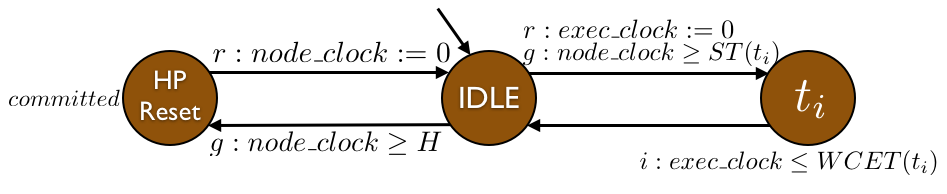
\includegraphics[width=0.75\textwidth]{img/generic_TA.png}
\caption{Basic timed automaton for a single task.}
\label{fig:generic_TA}
\end{figure}

\begin{figure}[thpb]
\centering
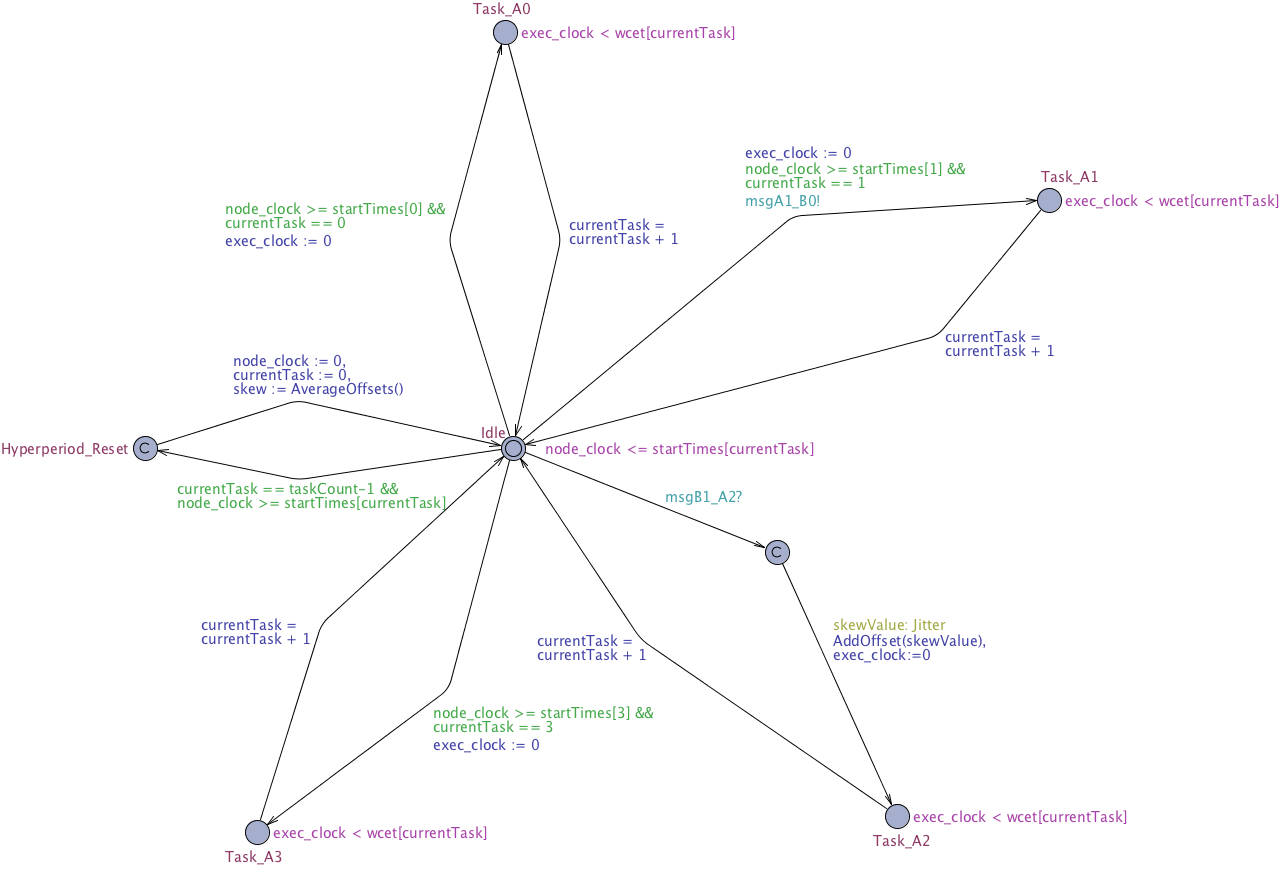
\includegraphics[width=0.75\textwidth]{img/uppaal_nodeA.png}
\caption{UPPAAL model of the task execution on a single processing node.}
\label{fig:uppaal_nodeA}
\end{figure}

The composition of synchronous tasks with a timed automata run-time layer results in complex system behavior that can alter the expected response as compared to a time-invariant controller\cite{gh_dissertation}.  Simulation and analysis of heterogenous models is non-trivial.  The BIP language and toolsuite are expressly designed to handle heterogeneity within a model and to provide support for simulation and analysis of such models\cite{bipref}.  In the supported work, we developed an extension to the ESMoL toolchain to support automated synthesis of models in the BIP language.  As an example, we illustrate the transformation of an ESMoL model's scheduler execution into first a timed automata for all of the tasks on the processing node (Fig. \ref{fig:uppaal_nodeA}) and finally into a BIP model for the interactions between the tasks which exchange messages on the bus (Fig. \ref{fig:task_model}).  Through these transformation our tools are able to utilize the model checking and simulation capabilities of both of these alternate formalisms.

\begin{figure}[thpb]
\centering
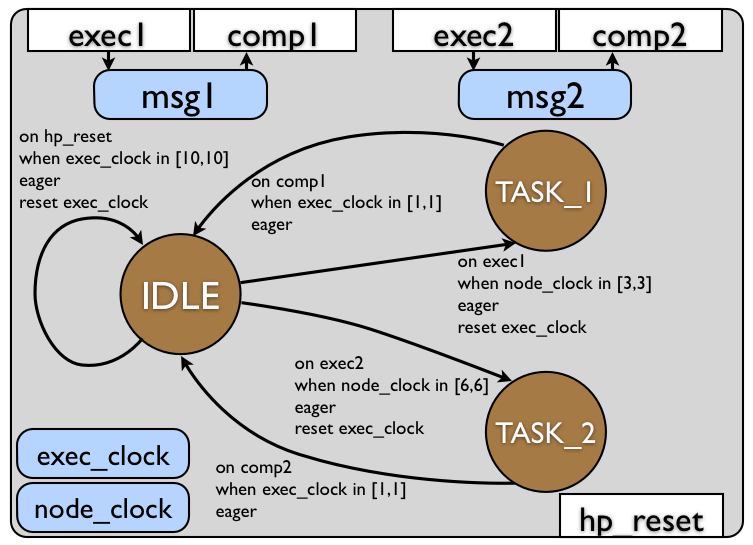
\includegraphics[width=0.75\textwidth]{img/task_model.png}
\caption{BIP model of tasks interacting indirectly by exchanging timed messages on the bus.}
\label{fig:task_model}
\end{figure}


\emph{ESMoL High-Confidence Design Tools}

The Embedded 
Systems Modeling Language (ESMoL) is a suite of 
domain-specific modeling languages (DSML) to integrate the 
disparate aspects of a safety-critical embedded systems design 
and maintain proper separation of concerns between control 
engineering, hardware specification, and software development 
teams\cite{jp_esmol}.  The Embedded Systems Modeling Language (ESMoL) encodes 
in models the relationships between controller functions
specified in Simulink, software components that implement
those functions (i.e. dataflow, messaging interfaces, 
etc\ldots), and the hardware platform on which the software
will run. The language and its associated tools provide the following capabilities:


\begin{itemize}

\item Provide a unified embedded software design environment 
so that modeling, analysis, 
simulation, and code generation artifacts are all 
clearly related to a single design model. ESMoL models use language-specified relations to associate Simulink 
control design structures with
software and hardware design concepts to define a
software implementation for controllers.

\item Include objects and parameters 
to describe deployment of software components to 
hardware platforms.  Analysis artifacts and simulation 
models generated from ESMoL models contain 
representations of the behavioral effects of the 
platform on the original design.

\item Integrate scheduling analysis
so that static schedules can be calculated in rapid design and
simulation cycles.  We include automatic generation of platform-specific
task configuration and data communications code in order to
rapidly move from modeling and analysis to testing on actual hardware.

\item Generate analysis models and code 
using simple template generation techniques.
Round-trip incorporation of calculated schedule 
analysis results back into the ESMoL model helps to
maintain consistency as models pass between design phases.

\end{itemize}

\begin{figure}[thpb]
\centering
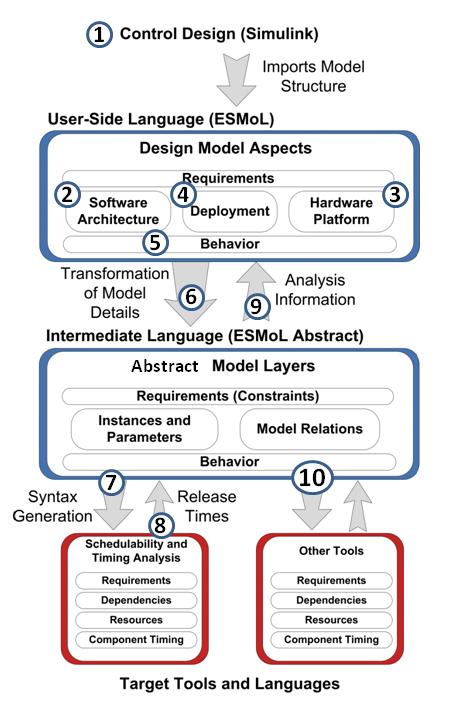
\includegraphics[width=0.75\textwidth]{img/designflow.png}
\caption{Design flow supported by the ESMoL tools.}
\label{fig:designflow}
\end{figure}

Fig. \ref{fig:designflow} illustrates the steps of the ESMoL design flow process\cite{jp_esmol}:

\begin{enumerate}
\item Import a Simulink controller design into an ESMoL model.
\item Specify software component functions and interfaces, and instantiate the components into a logical software architecture model.  At this point functional code generation can take place.
\item Specify the hardware topology for a time-triggered distributed processing network.
\item Define the logical dataflow between software component instances, and the deployment of the logical dataflow to the hardware.
\item Give timing parameters for the tasks and messages in the system.
\item Transform the ESMoL model into a flattened model (ESMoL\_Abstract), resolving all implied model relationships.
\item Transform the ESMoL\_Abstract model into analysis models (such as scheduling problem specifications). Run the analysis.
\item Import results from the analysis back into the ESMoL\_Abstract for consumption by other tools.
\item Import results from the analysis in the ESMoL model (for the user).
\item Generate platform-specific simulations and deployable code from ESMoL\_Abstract.
\end{enumerate}

The control design models provide task period configurations, and 
either profiling or static analysis provides worst-case 
execution time parameters for each component instance.  
Data transfer rates and overhead parameters for communication
buses are stored in the platform model. \cite{jp_tt_sched}
describes the mapping of model structure, execution information,
and platform parameters into actual constraint model details. The Gecode constraint programming
tool solves these constraints for task release and
message transfer times on the time-triggered platform. The scheduling process
should guarantee that the implementation meets the timing requirements 
required by the control design process.

\begin{table*}
\centering
\begin{alltt}
Resolution 1ms

Proc RS 4MHz 0s 0s
Comp InnerLoop =50Hz 1.9ms
Comp DataHandling =50Hz 1.8ms
Comp SerialIn =50Hz 1us
Comp SerialOut =50Hz 1ms
Msg DataHandling.sensor_data_in 1B RS/SerialIn RS/DataHandling 
Msg InnerLoop.thrust_commands 37B RS/InnerLoop RS/SerialOut
Msg DataHandling.ang_msg 1B RS/DataHandling RS/InnerLoop 

Proc GS 100MHz 0s 0s
Comp RefHandling =50Hz 1us
Comp OuterLoop =50Hz 245us
Msg RefHandling.pos_ref_out 9B GS/RefHandling GS/OuterLoop 

Bus TT_I2C 100kb 1.3ms
Msg OuterLoop.ang_ref 20B GS/OuterLoop RS/InnerLoop 
Msg DataHandling.pos_msg 8B RS/DataHandling GS/OuterLoop 
\end{alltt}
\caption{Scheduling spec for the Quadrotor example.}
\label{code:qr_spec}
\end{table*}

\begin{table*}
\centering
\begin{alltt}
\scriptsize
Resolution \{\{RESOLUTION\}\}

\{\{\#HOST_SECTION\}\}Proc \{\{NODENAME\}\} \{\{NODEFREQ\}\} \{\{SENDOHD\}\} \{\{RECVOHD\}\}
\{\{\#TASK_SECTION\}\}Comp \{\{TASKNAME\}\} =\{\{FREQUENCY\}\} \{\{WCEXECTIME\}\}
\{\{\/TASK_SECTION\}\}\{\{\#LOCAL_MSG_SECTION\}\}Msg \{\{MSGNAME\}\} \{\{MSGSIZE\}\} \{\{SENDTASK\}\} \{\{RECVTASKS\}\}
\{\{\/LOCAL_MSG_SECTION\}\}
\{\{\/HOST_SECTION\}\}
\{\{\#BUS_SECTION\}\}Bus \{\{BUSNAME\}\} \{\{BUSRATE\}\} \{\{SETUPTIME\}\} \{\{\#BUS_HOST_SECTION\}\}\{\{NODENAME\}\} \{\{\/BUS_HOST_SECTION\}\}
\{\{\#MSG_SECTION\}\}Msg \{\{MSGNAME\}\} \{\{MSGSIZE\}\} \{\{SENDTASK\}\} \{\{RECVTASKS\}\}
\{\{\/MSG_SECTION\}\}
\{\{\/BUS_SECTION\}\}
\{\{\#LATENCY_SECTION\}\}Latency \{\{LATENCY\}\} \{\{SENDTASK\}\} \{\{RECVTASK\}\}
\{\{\/LATENCY_SECTION\}\}
\end{alltt}
\caption{Stage 2 Interpreter Template for the Scheduling Specification}
\label{code:sched_templ}
\end{table*}

Scheduling specifications are created in the Stage 2 interpreter from
the template shown in Table \ref{code:sched_templ}.
The Stage 2 scheduler generation logic traverses the 
ESMoL\_Abstract model and fills in the structures
which are used to fill in the template when the 
CTemplate generator is invoked.  
In CTemplate, each \verb${{#...}} {{/...}}$ tag pair delimits a 
section which can be repeated by filling in the proper data 
structure in the code.  The other tags \verb${{...}}$ are 
replaced by the string specified in the generation code. 

Producing the \emph{Proc} and \emph{Comp} lines from the model 
API is straightforward as the output mirrors the model
hierarchy, so these lines require only simple traversals 
of the model.  Each generated line uses parameters 
from the respective model object to fill in the blanks.  

In the consraint problem, our scheduler makes use of a global serialization constraint to represent non-preemption\cite{jp_tt_sched}.  The global serialization constraint forces all variable assignments from the given set to be distinct, and to differ by at least a constant value (duration).  For efficiency (and model conciseness), global distinctness constraints are used instead of $n^2$ constraints representing all possibilities.  The scheduler performed well on
randomized problem sets with respect to both execution time and memory usage.

\begin{figure}[thpb]
		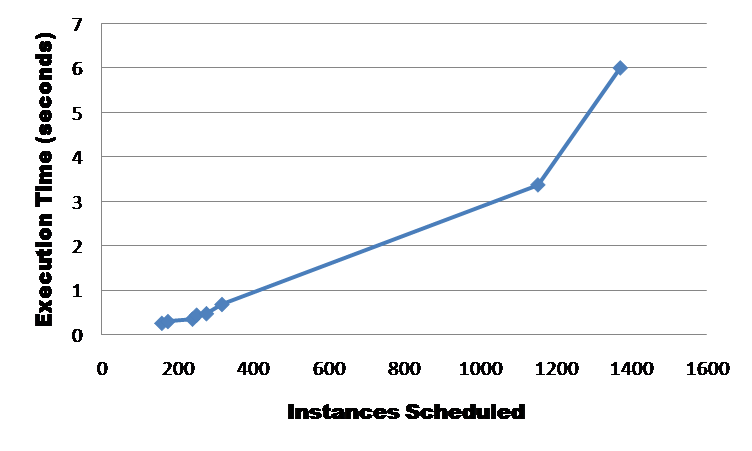
\includegraphics[scale=.7]{img/exectime.png}
		\centering
		\caption{Execution time for feasible instances.}
	  \label{fig:exectime}
\end{figure}

\begin{figure}[thpb]
		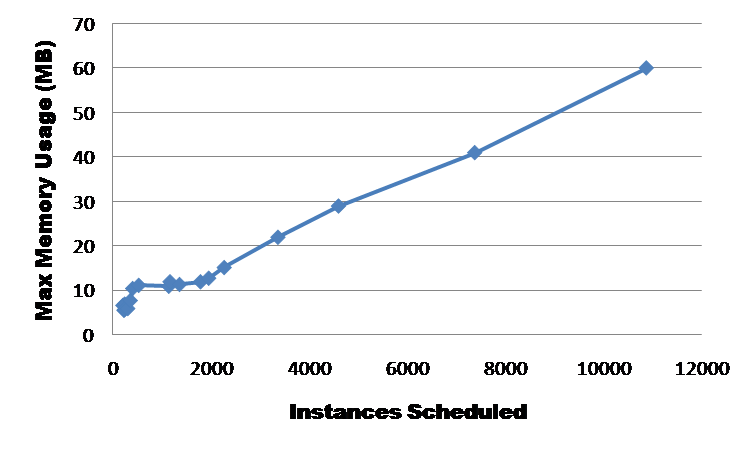
\includegraphics[scale=.7]{img/memusage.png}
		\centering
		\caption{Maximum memory consumption vs. problem instance size.}
		\label{fig:memusage}
\end{figure}

\emph{FRODO Portable Time-Triggered Runtime}

The experimental platform includes a Linux-based TTA realization (the FRODO TTA virtual
machine, running on a low-end ARM Linux board, called the Gumstix platform) and an RTOS-based
TTA realization (the same virtual machine, running on a low-end AVR board, called
the Robostix platform). The same hardware platforms are used in one version of the STARMAC quadrotor.
We have developed platform-specific code generators that create task and communication wrappers for functional
code which will run on the FRODO VM.  We also create I/O drivers for the low-end controller that work with the
time-triggered run-time scheduler and can be targeted by the generators. 

Our tools also implement the FRODO TTA virtual machine logic and timing directly on the TrueTime kernel using the C++ API, to ensure that the platform-included TrueTime model has the same execution semantics as the FRODO runtime on the target hardware\cite{gh_truetime}. 
The TrueTime interface makes the high-fidelity simulation based analysis of controller designs feasible. The actual functional code and the actual schedule are used in the analysis; hence the platform effects are directly observable.  Observations on this simulation provide valuable feedback for the designer on how well the actual controller implementation will work in the real environment. Once the design is found satisfactory, the code can be generated and deployed on the actual controller platform and its performance studied using a hardware-in-the-loop simulation.
Validation of the TrueTime models for the quadrotor uncovered the existence of extra time delay states in the target hardware implementation due to double-buffering on the sensor data receiver.  The TrueTime model was updated to account for the buffer delay.


\begin{figure}[thpb]
\centering
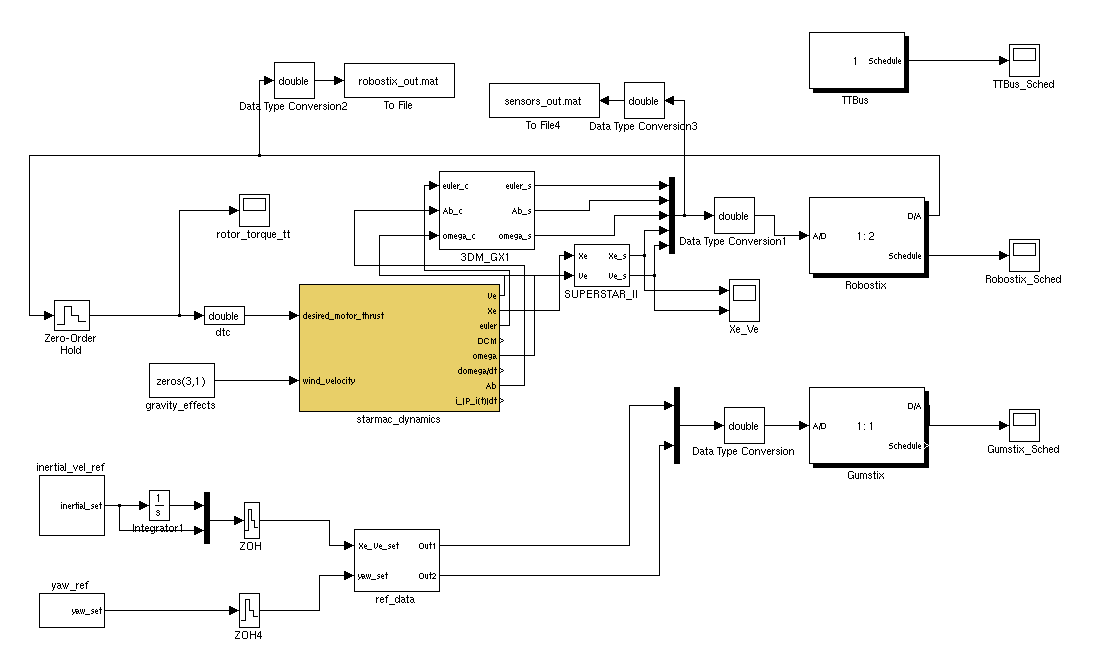
\includegraphics[width=0.9\textwidth]{img/qr_tt}
\caption{TrueTime model of the Starmac quadrotor, including the processor execution timing effects and data networking.}
\label{fig:qr_tt}
\end{figure}



\emph{Other Relevant Tools and Techniques for Design Evaluation}

We have a prototype integration of the CMU statistical model checking tools with our STARMAC model to analyze the robustness of our design to fault conditions.  We give a simple example to illustrate the use of statistical model checking in the quadrotor model.  Fig. \ref{fig:fault1} depicts a fault scenario where the height sensor data includes intermittent (and frequent) glitches which are orders of magnitude larger than the valid data samples (center of the figure).  The traces of the simulated velocity trajectory (right) show that the change in quadrotor height over time has become noisy.  The noise is further aggravated by time delays introduced in the distributed implementation of the controller (lower right).  We would like to formally pose the question of whether the faulty sensor has destabilized the controller and/or its implementation. 

\begin{figure}[thpb]
\centering
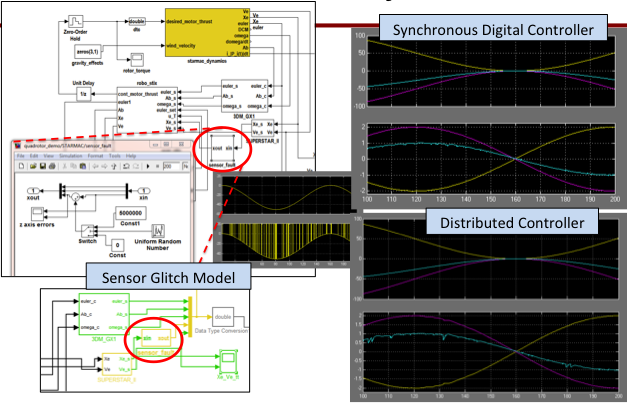
\includegraphics[width=0.9\textwidth]{img/FaultModeling}
\caption{Injection of an aggravated sensor spike fault into the quadrotor behavior. We need to see whether this fault
 causes instability in the distributed deployment of the controller software.}
\label{fig:fault1}
\end{figure}

Fig. \ref{fig:fault2} shows the model framework in Simulink for the use of the Bayesian statistical model checking
\cite{PZ_smc} to evaluate the stability of the control loop with the fault included. The MFOTL block implements 
the interface of the model checker with the Simulink runtime.  The model checking block is configured with an LTL 
condition ``F[0,100s] f1 > 250''.  This sets a hard threshold within which the quadrotor's height must remain during the time specified (100 seconds). A script (bottom of Fig. \ref{fig:fault2}) repeatedly runs the simulation and collects statistics on whether the simulated quadrotor with faulty behavior has destabilized the system. 
In statistical model checking, scalability is still a major issue. We were able to achieve 90\% confidence for this test case in 19 minutes on a 2 GHz processor, but 99\% confidence required 156 minutes.

\begin{figure}[thpb]
\centering
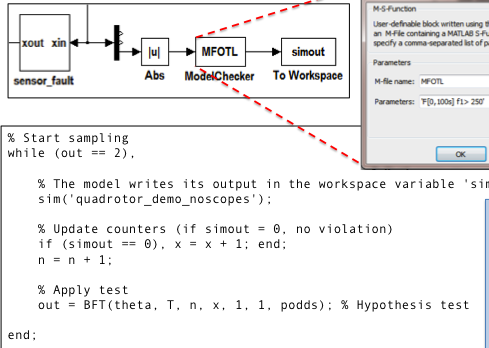
\includegraphics[width=0.9\textwidth]{img/FaultModeling2}
\caption{Addition of the integrated model-checking block, together with the safety condition and execution script.}
\label{fig:fault2}
\end{figure}

We have created prototype extensions to the ESMoL language to support design flows (Fig. \ref{fig:fault3}) which capture the details of fault scenarios and test cases which evaluate those scenarios (Fig. \ref{fig:fault4}).  The intent is to model faulty behavior separately from the nominal design, and to generate statistical model checking simulations as needed which include fault behaviors, conditions, and inputs.

\begin{figure}[thpb]
\centering
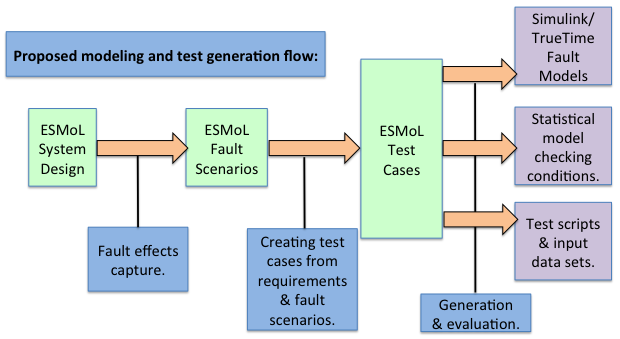
\includegraphics[width=0.9\textwidth]{img/FaultModeling3}
\caption{Proposed design flow to be supported by ESMoL language extensions for fault modeling and testing.}
\label{fig:fault3}
\end{figure}


\begin{figure}[thpb]
\centering
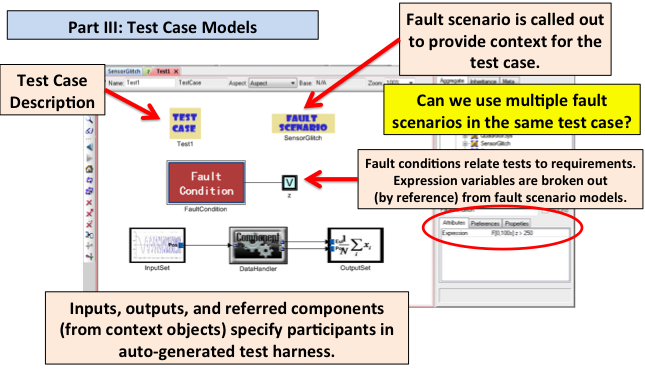
\includegraphics[width=0.9\textwidth]{img/FaultModeling4}
\caption{Test bench language prototype for ESMoL. This concept has been successfully implemented in the CyPhyML system design language and tools (DARPA AVM META project).}
\label{fig:fault4}
\end{figure}



\emph{Pluggable Interpreter Development Architecture}

Fig. \ref{fig:designflow} depicts a design flow 
that includes a user-facing modeling language 
for design and an abstract intermediate language 
for supporting interpreter development and
maintenance.  In our tools, a completed ESMoL model is 
transformed via the Stage 1 
transformation into a model in the ESMoL\_Abstract 
language, where all implied relationships and structural 
model inferences have been resolved (Fig. \ref{fig:stage1}).  
The first model transformation 
flattens the user model into the abstract intermediate form,
translating parameters and resolving special cases as needed. 
Model interpreters 
for calculating time-triggered schedules, creating 
platform-specific simulations, and generating deployable 
code are integrated using the Stage 2 transformation (Fig. \ref{fig:stage2}).
Because generators for code and analysis are attached to the abstract 
modeling layer, so the simpler second-stage transformations 
are easier to maintain, and are isolated from changes to 
the user language and tools.

\begin{figure}[thpb]
\centering
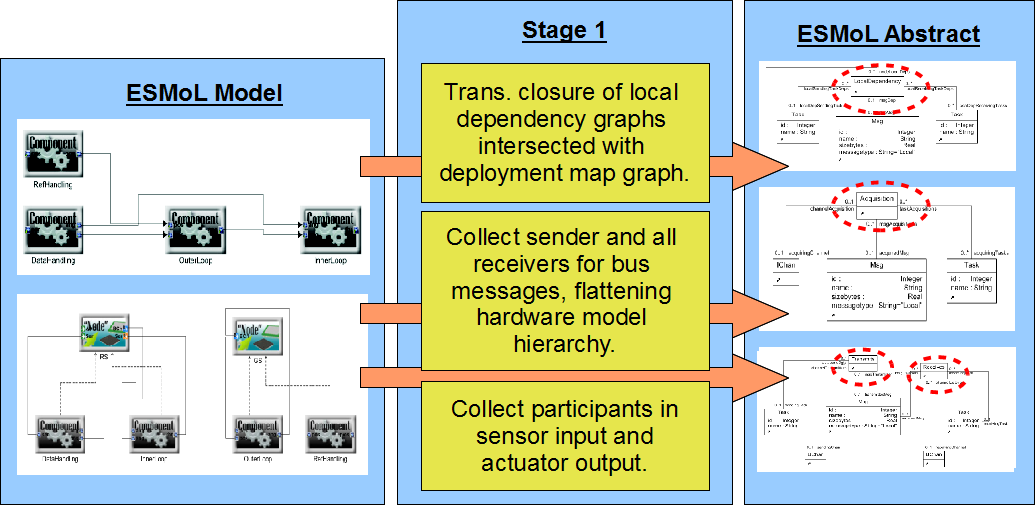
\includegraphics[width=0.9\textwidth]{img/stage1}
\caption{Stage 1 of the ESMoL interpreter framework, which resolves structural inferences and creates a flattened deployment model.}
\label{fig:stage1}
\end{figure}

\begin{figure}[thpb]
\centering
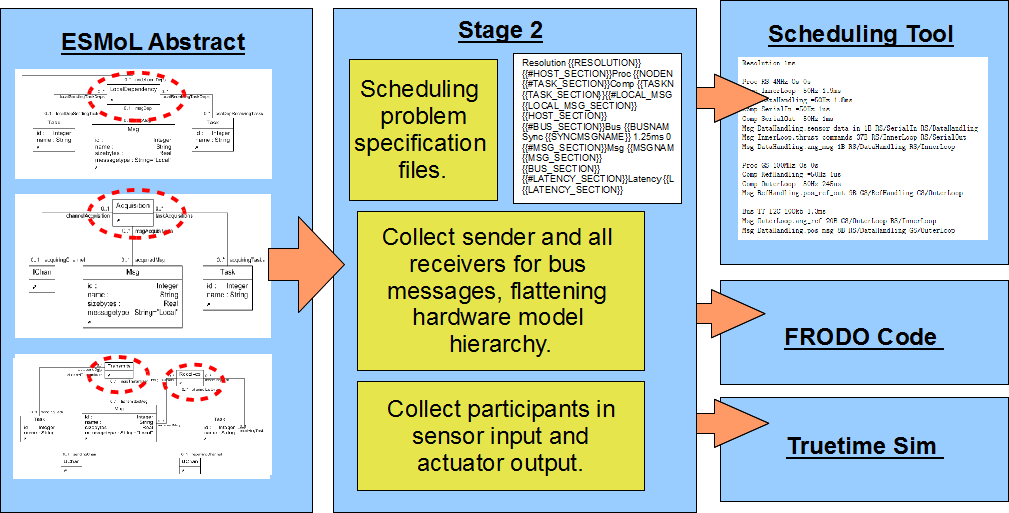
\includegraphics[width=0.9\textwidth]{img/stage2}
\caption{Stage 2 of the ESMoL interpreter framework, which performs the actual transformations. A SystemC target is currently under development for detailed hardware design and evaluation.} 
\label{fig:stage2}
\end{figure}

In the model integrated computing approach, domain specific 
modeling languages represent different aspects of the design, 
with the aim  of consistently integrating different concepts 
and details for those design aspects and integrated analysis tools.
This architecture makes interpreter development simpler, extending the language composition
capabilities of the MIC tools with greater composability for modeling language tools as well.
Fig. \ref{fig:sched_integration} depicts the details of one example of such a
transformation, the schedule problem generation described previously.

\begin{figure}[thpb]
\centering
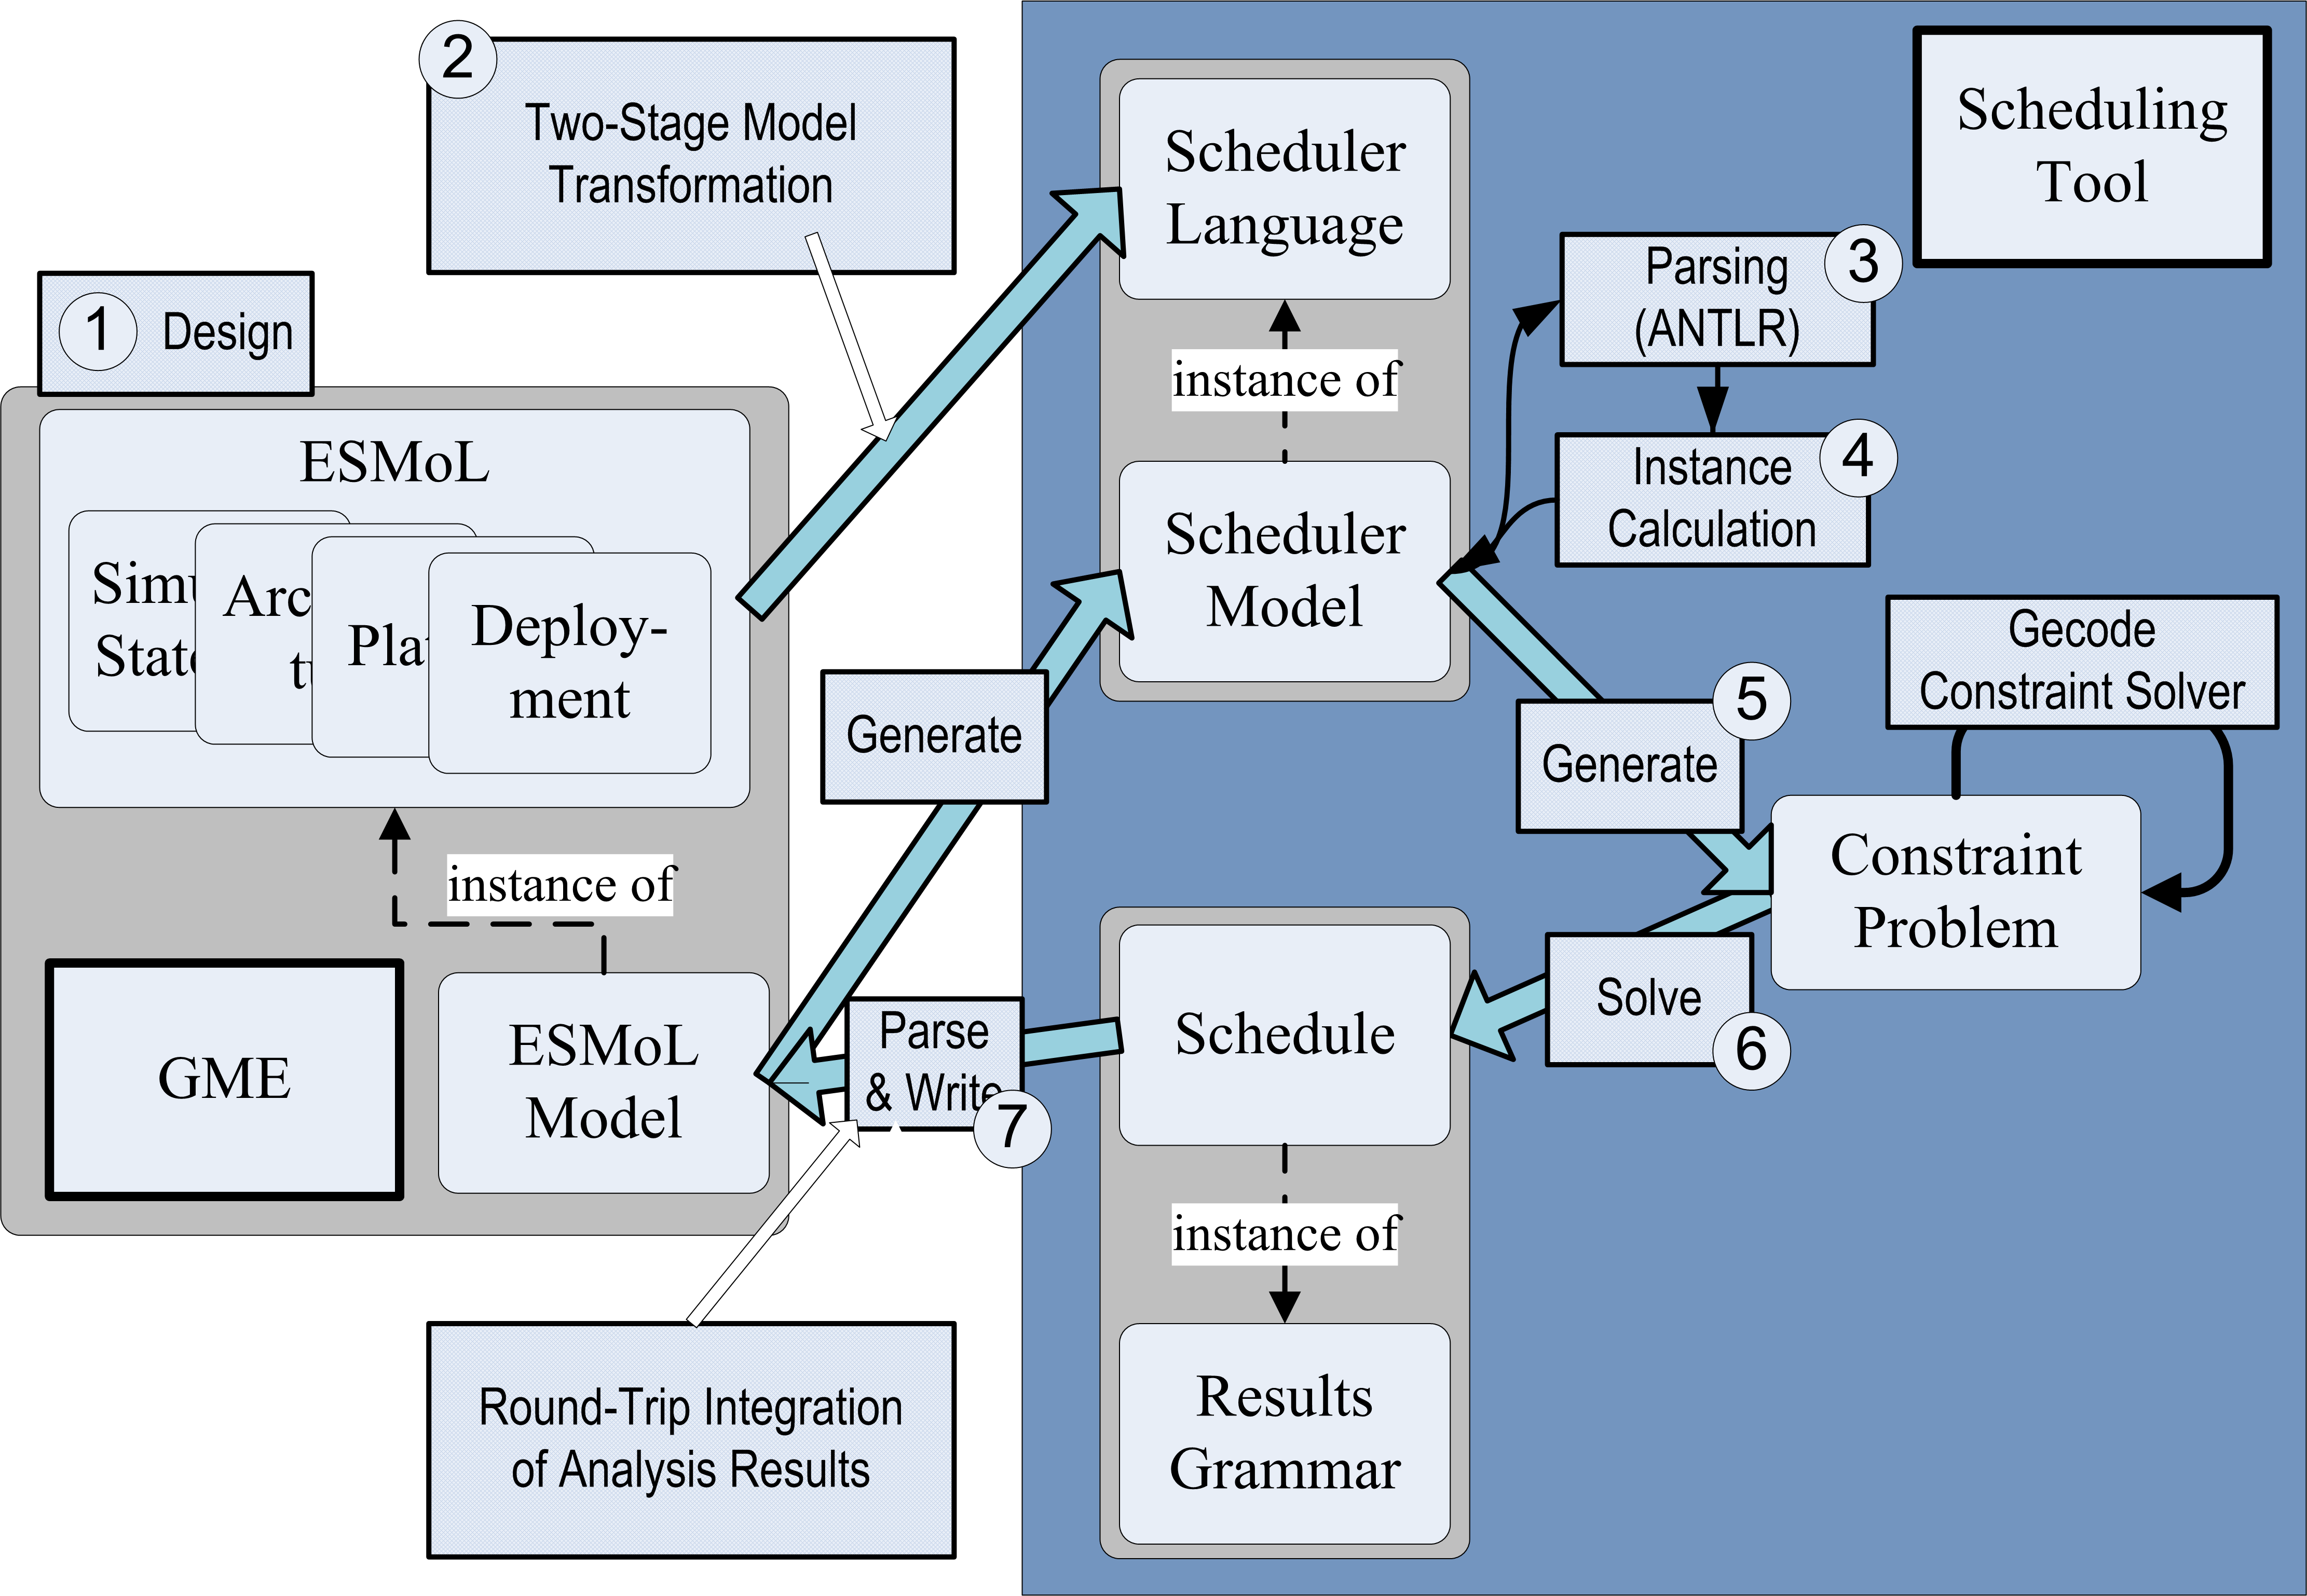
\includegraphics[width=0.9\textwidth]{img/sched_integration}
\caption{Example: Stage 2 generates scheduling problem specifications using the Stage 1 results and output templates. Results are parsed and written back into the source model.} 
\label{fig:sched_integration}
\end{figure}


\subsubsection{Controlling Timing with a deadline instruction (Lee)}

	      
	      We have enabled control over timing at the ISA level by
               introducing four so-called ``deadline''
               instructions. As higher-level models of computation
               (MoC) often have a timed semantics, the deadline
               instructions can be used to implement such MoCs at the
               binary level, thereby filling a void in the model-based
               development of high-confidence systems from high-level
               models to low-level realizations. To allow for a wide
               range of cost-efficient implementations of the PRET
               timed semantics, it can be parameterized in different
               architectural aspects, as for instance the sizes of
               different levels of the memory hierarchy. We have made
               significant progress in developing parametric timing
               analyses to support the verification of timing
               constraints on PRET.

               On the implementation side, we have continued the
               development of a prototypical PRET processor called
               PTARM, implementing the four deadline instructions and
               providing predictable timing behavior. A new PRET DRAM
               controller provides access to large Dynamic RAMs at
               predictable and composable memory access times to the
               four hardware threads of the PTARM core. Compared with
               previous approaches, we improve the worst-case access
               latency of small requests by up to 73\%.
               
               Report:
               
               Guaranteeing the correct behavior of embedded systems
               is extremely difficult, especially with respect to
               timing constraints and their relationship to the safety
               of the physical systems. The traditional verification
               process is faced with two major challenges regarding
               timing constraints: 1. The execution time of a program
               depends on the hardware on which it is running. Every
               new hardware realization requires the development of
               new timing analysis tools. 2. The development process
               of such analysis tools is becoming increasingly
               error-prone and time-consuming for modern, complex
               hardware realizations.

               PRET tackles both of these challenges. By introducing a
               timed semantics for the instruction set architecture,
               timing becomes a property of programs rather than a
               property of programs running on particular hardware
               realizations. As a consequence, programs can be ported
               from one realization to the next without having to
               recertify and develop new timing analysis
               tools. Furthermore, due to the simplicity of the timing
               model associated with the ISA, precise and efficient
               timing analysis becomes possible. We anticipate this
               work to entail a paradigm shift in the development of
               hardware realizations for embedded systems: instead of
               focusing on improving performance, new hardware
               realizations will be developed that optimize aspects
               such as energy and power consumption, implementation
               cost, and reliability.

               In the past year, we have taken the following steps towards the PRET vision: 
               \begin{itemize}

               \item We have introduced four so-called ``deadline''
                 instructions, which introduce control over timing
                 at the ISA level. These instructions allow to
                 enforce upper and lower bounds on the execution
                 time of blocks of code and provide the ability to
                 act upon deadline misses. As higher-level models of
                 computation (MoC) often have a timed semantics, the
                 deadline instructions can be used to implement such
                 MoCs at the binary level, thereby filling a void in
                 the model-based development of high-confidence
                 systems from high-level models to low-level
                 realizations. This work
                 \cite{Reineke11_PRETDRAMControllerBankPrivatizationForPredictability}
                 has been presented at DAC 2011.

               \item We have continued the development of a
                 prototypical PRET processor called PTARM, which
                 shall implement the four deadline instructions and
                 provide predictable timing behavior \cite{LiuReinekeLee10_PRETArchitectureSupportingConcurrentProgramsWithComposable}.

               \item We have developed a new DRAM controller which
                 provides predictable and composable memory access
                 times to the four hardware threads of the PTARM
                 core. Instead of viewing the DRAM device as one
                 resource that can only be shared as a whole, our
                 approach views it as multiple resources that can be
                 shared between one or more clients individually. We
                 partition the physical address space following the
                 internal structure of the DRAM device, i.e., its
                 ranks and banks, and interleave accesses to the
                 blocks of this partition. This eliminates
                 contention for shared resources within the device,
                 making accesses temporally predictable and
                 temporally isolated. Compared with previous
                 approaches, we improve the worst-case access
                 latency of small requests by up to 73\%. This work
                 \cite{Reineke11_PRETDRAMControllerBankPrivatizationForPredictability},
                 has been presented at CODES+ISSS 2011.

               \item To allow for a wide range of cost-efficient
                 implementations of the PRET timed semantics, it can
                 be parameterized in different architectural
                 aspects, as for instance the sizes of different
                 levels of the memory hierarchy and their respective
                 latencies, or the latencies floating-point
                 instructions. Supporting such a parameterized timed
                 semantics requires parametric timing
                 analysis. Parametric timing analysis derives a
                 predicate that is satisfied for choices of
                 parameter values that are guaranteed to meet all
                 timing constraints. This summer, we have made
                 significant progress in developing such parametric
                 analyses.

               \end{itemize}



\subsection{Testing and Experimental Validation (Tomlin, Sastry, Lee, Karsai)}


The project team collaborated to create a Starmac simulation model, which was published on the web site. It was released as an example in the ESMoL tool distribution as well\cite{jp_esmol}.  Gabe Hoffman (Stanford) produced the original Starmac model in Simulink (Fig. \ref{fig:starmac_mdl}), which was later revised by Jim Kapinski (CMU) and then Nicholas Kottenstette (Vanderbilt).  The Vanderbilt team added passive controllers in the same architectural framework 
as the original Starmac controllers (Fig. \ref{fig:starmac_arch}).

\begin{figure}[thpb]
\centering
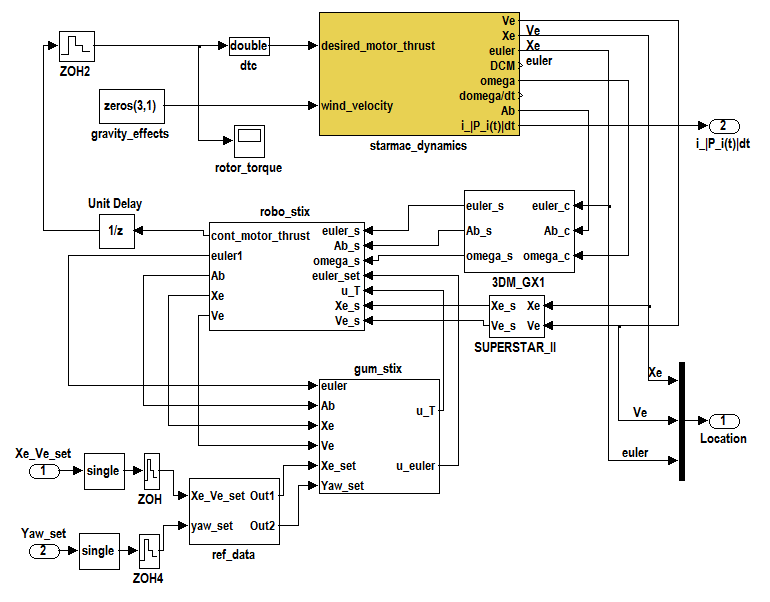
\includegraphics[width=0.9\textwidth]{img/real_quadrotor_mdl.png}
\caption{Simulink model of the Starmac quadrotor.}
\label{fig:starmac_mdl}
\end{figure}

\begin{figure}[thpb]
\centering
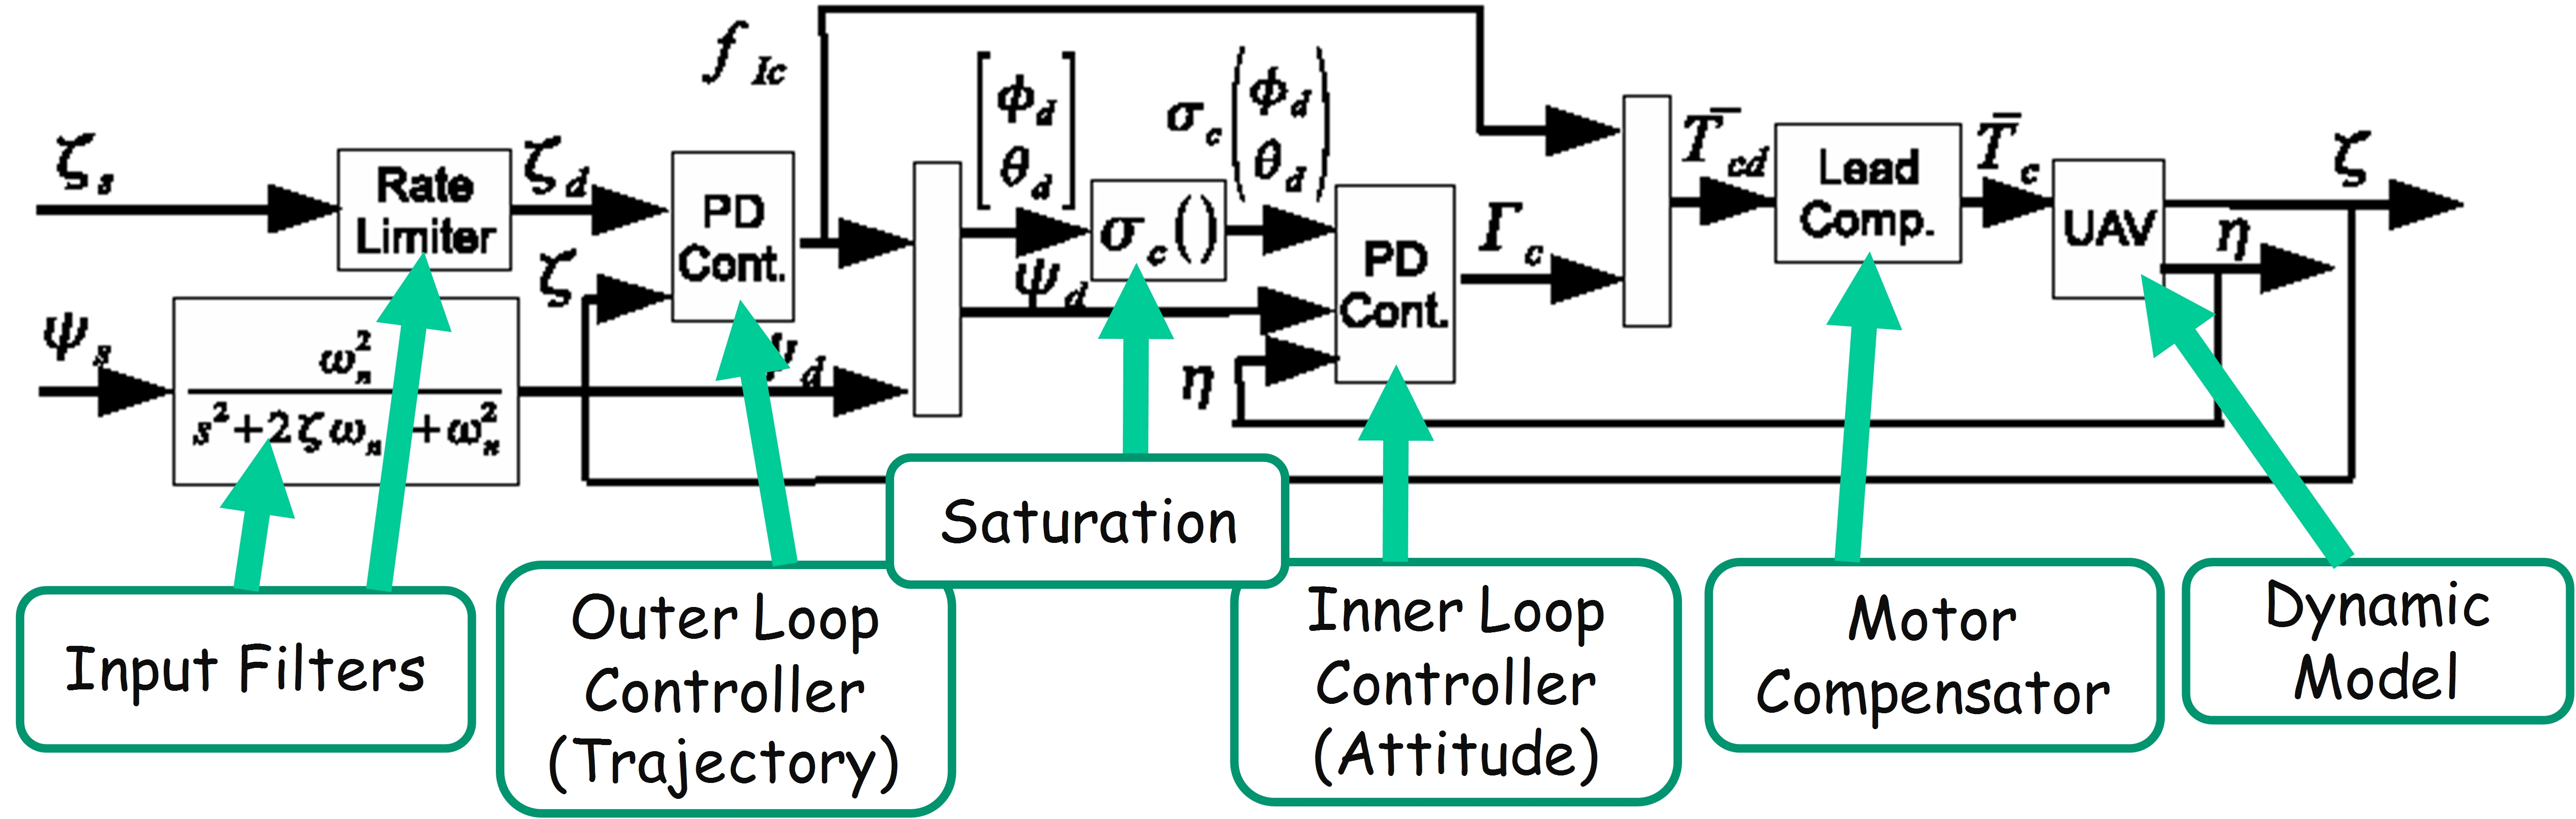
\includegraphics[width=0.9\textwidth]{img/quadrotor_arch.png}
\caption{Controller architecture for the quadrotor.}
\label{fig:starmac_arch}
\end{figure}

Beyond the evaluation in TrueTime described above, we also created a hardware-in-the-loop (HIL) experimental testbed to validate the controller code against the TrueTime models\cite{gh_truetime,nk_qr_tr,jp_dissertation}..
Fig. \ref{fig:hil_setup} contains the structure of the HIL experiment setup.  The xPC target software runs the quadrotor dynamics, and the actual Gumstix and Robostix processors run the passive controllers.  The interface between the plant simulator and the controller is ‘hard real-time’, and the xPC box simulates the real-time behavior of the plant with high-fidelity (e.g., inner loop control can be easily run at 100Hz).  The control software is generated and con-figured with the tool chain. Trajectories of the HIL-simulated controller appear in Fig. \ref{fig:starmac_hil}.

\begin{figure}[thpb]
\centering
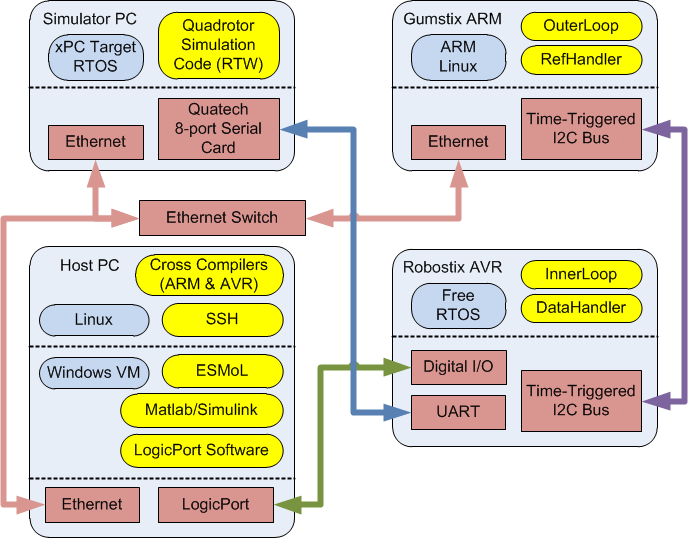
\includegraphics[width=0.9\textwidth]{img/hil_setup.png}
\caption{Overview of the hardware-in-the-loop simulation configuration.}
\label{fig:hil_setup}
\end{figure}


\begin{figure}[thpb]
\centering
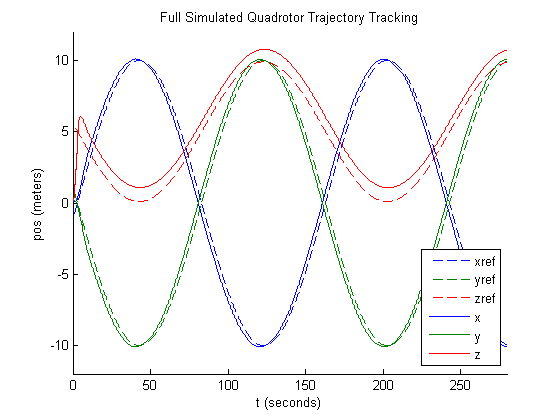
\includegraphics[width=0.9\textwidth]{img/qr_tracking.png}
\caption{Trajectory tracking for the passive controller code running in a hardware-in-the-loop simulation of the Starmac dynamics.}
\label{fig:starmac_hil}
\end{figure}


\emph{Online sector analysis}

We developed a moethod for comparing the stability criteria between the simulated quadrotor and its realization on the distributed network.
To illustrate the principle we used a continuous-time system whose model represents a simplified version of the quadrotor UAV.   This model still follows the  
basic component architecture for the control design (see Fig. \ref{fig:starmac_arch}), but excludes the nonlinear rotational 
dynamics of the full quadrotor while retaining
the difficult coupled stability characteristics.The 
example model controls a stack of four integrators (and motor lag) 
using two nested PD control loops.The two control loops (\emph{InnerLoop} and \emph{OuterLoop},
are deployed to the Robostix and Gumstix
processors, respectively, exactly as in the Starmac.  We refer to this example as the Quad Integrator model.  All of the controller components run at a frequency of 50Hz.  


Our controller evaluation method is based on sector theory, proposed originally by Zames to analyze nonlinear elements in a control design.  Sectors provide two real-valued parameters which represent bounds on the possible input/output behaviors of a control loop.  Kottenstette presented a sector analysis block for validating a control design in Simulink\cite{nk_qr_tr}.  We propose to use the same structure to verify the deployed quadrotor control software online.  This method is described more fully in Porter et al\cite{jp_online_stability}.  A few concepts make this approach appealing for our case:

\begin{enumerate}
 \item For a given component, the sector measures behavior simultaneously over multiple inputs and outputs, so only one sector analyzer is required per control loop.
 \item Our passive abstraction of the system design (described below) allowed us to use a sector analyzer for each control loop to quickly isolate problem components in the deployed design.
\end{enumerate}

Passive control requires that controllers use energy received from inputs or stored previously, introducing no new energy into the environment. If the plant dynamics were passive, we would have considerable freedom in setting gains and choosing control structures.  The zero-order hold outputs can introduce small amounts of new energy to the environment during rapid velocity changes, so each of the control loops must mitigate small amounts of ``active'' behavior.  The sector bound $a$ quantifies the energy-generating behavior of each control loop. In our quadrotor system, we expect the bound $a$ to be small and negative and choose the gains appropriately.  The result from Kottenstette indicates that the condition $k < -1/a$ is sufficient to ensure stability in these situations (where $k$ is the configured gain of the control loop)\cite{nk_qr_tr}.

\begin{figure*}[thpb]
\centering
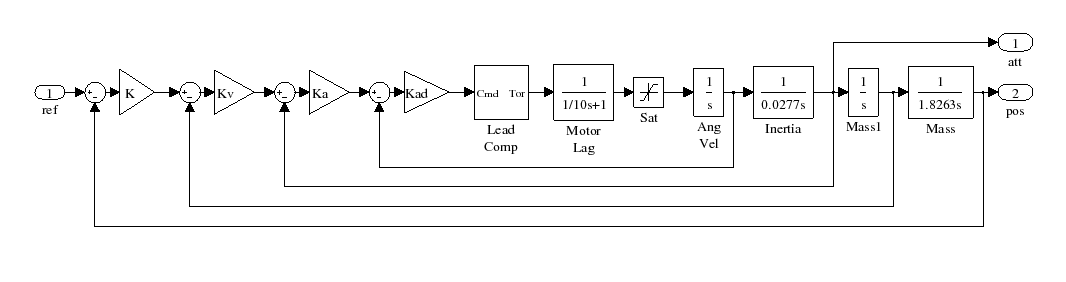
\includegraphics[width=\columnwidth]{img/quadrotor_loops}
    \caption{Conceptual nested loop structure of the controller.}
    \label{fig:quadrotor_loops}
\end{figure*}

This particular design must be evaluated from the innermost loop to the outermost loop in order to make sense of the gain constraints. Fig. \ref{fig:quadrotor_loops} shows the nested loop structure of the design.  The actual design and implementation are complicated by the physical architecture of the digital realization: 

\begin{enumerate}
 \item Sensors acquire digital attitude and position information only, so velocities must be estimated.
 \item The controller components are deployed to different processors in the digital implementation, as described previously. Components on the two processors exchange data messages using a time-triggered protocol.
 \item Motor thrust commands are issued periodically using a zero-order hold.  As discussed previously the hold introduces additional energy back into the environment, violating the passivity condition.
\end{enumerate}

The sector blocks are attached around each controller, so input and output ports are oriented from the point of view of the control element.  The output of the controller (input to the rest of the system) is connected to the sector analyzer input port.  The signal controlled by the controller (before the error term is formed) is part of the input to the controller, but from our point of view it is the output of the system, so it connects to the sector
analyzer output port.  Fig. \ref{fig:sectorconn} displays the connection of the sector search block around the position control gain for our example. $K_x$ is the proportional gain for the outer loop PD controller, and $K_v$ is the derivative gain.  

\begin{figure}[thpb]
\centering
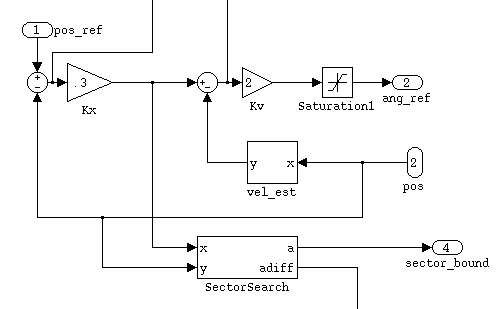
\includegraphics[width=0.75\columnwidth]{img/sectorconn}
    \caption{Sector analysis block (\emph{SectorSearch}) connection around the position controller.}
    \label{fig:sectorconn}
\end{figure}



\begin{figure}[thpb]
\centering
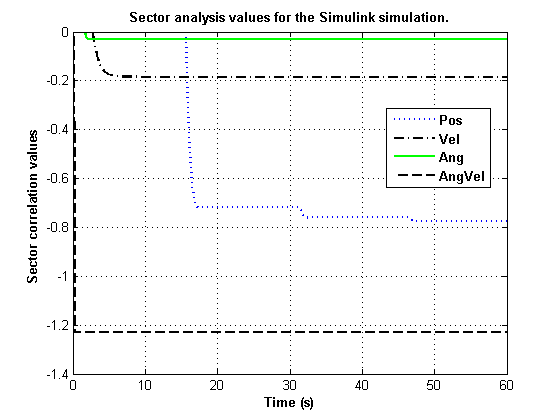
\includegraphics[width=0.75\columnwidth]{img/simsectors}
\caption{Sector value evolution over time for the quad integrator (Simulink only).}
\label{fig:sectors1} 
\end{figure}

\begin{figure}[thpb]
\centering
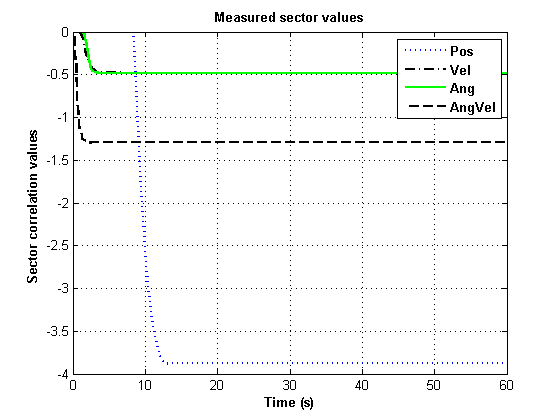
\includegraphics[width=0.75\columnwidth]{img/meassectors}
\caption{Sector value evolution over time for the quad integrator (Hardware-in-the-loop).}
\label{fig:sectors2} 
\end{figure}



\begin{table*}[thpb]
\centering

\begin{tabular}[width=0.95\columnwidth]{ | l | l | l | l | l | l | l | }

\hline
\textbf{Signal} & \textbf{Original} & \textbf{Simulated} & \textbf{Measured} & \textbf{Delta} & \textbf{New} & \textbf{New} \\
                & \textbf{Bound}    & \textbf{Sector}    & \textbf{Sector}  &                & \textbf{Bound} & \textbf{Sector} \\
\hline \hline
Angular  & -1.333 & -1.2292 & -1.2963 & -0.0671 & -2.667 & -1.4568 \\
Velocity & & & & & & \\
\hline
Angle & -0.5 & -0.0295 & -0.4831 & -0.4536 & -1.0 & -0.0068 \\
\hline
Velocity & -0.5 & -0.1856 & -0.4830 & -0.2974 & -1.0 &  -0.9324 \\
\hline
Position & -3.333 & -.7757 & -3.8811 & -3.1054 & -6.667 & -1.6081 \\
\hline
\end{tabular}
\caption{Sector value comparisons for simulation and execution on the actual platform.}
\label{tab:sectors}
\end{table*}






               \section{\textsf{Participants}}

               \subsection{Vanderbilt}

               \begin{indentation}{0pt}{0pt}{0pt}
                 \uppercase{PRINCIPAL INVESTIGATOR:}
               \end{indentation}
               
               \begin{indentation}{36pt}{0pt}{0pt}
                 Janos Sztipanovits (Faculty)
               \end{indentation}

               \begin{indentation}{0pt}{0pt}{0pt}
               \end{indentation}

               \begin{indentation}{0pt}{0pt}{0pt}
                 \uppercase{CO-PRINCIPAL INVESTIGATORS:}
               \end{indentation}

               \begin{indentation}{36pt}{0pt}{0pt}
                 Gabor Karsai (Faculty)
               \end{indentation}

               \begin{indentation}{0pt}{0pt}{0pt}
               \end{indentation}

               \begin{indentation}{0pt}{0pt}{0pt}
                 \uppercase{GRADUATE STUDENTS:}
               \end{indentation}

               \begin{indentation}{0pt}{0pt}{0pt}
               \end{indentation}

               \begin{indentation}{36pt}{0pt}{0pt}
                 Graham Hemingway (Graduate Student, partially funded)
               \end{indentation}

               \begin{indentation}{36pt}{0pt}{0pt}
                 Joseph Porter (Graduate Student, partially funded)
               \end{indentation}

               \begin{indentation}{0pt}{0pt}{0pt}
                 \uppercase{STAFF:}
               \end{indentation}

               \begin{indentation}{0pt}{0pt}{36pt}
                 Nicholas Kottenstette (Research Scientist, partially funded)
               \end{indentation}

               \begin{indentation}{0pt}{0pt}{36pt}
                 Chris VanBuskirk (Research Scientist, partially funded)
               \end{indentation}

               \begin{indentation}{0pt}{0pt}{36pt}
                 Harmon Nine (Senior Staff Engineer, supported elsewhere)
               \end{indentation}


               \subsection{UC Berkeley}

               \begin{indentation}{0pt}{0pt}{0pt}
                 \uppercase{PRINCIPAL INVESTIGATOR:}
               \end{indentation}
               
               \begin{indentation}{36pt}{0pt}{0pt}
                 Claire Tomlin
               \end{indentation}

               \begin{indentation}{0pt}{0pt}{0pt}
               \end{indentation}

               \begin{indentation}{0pt}{0pt}{0pt}
                 \uppercase{CO-PRINCIPAL INVESTIGATORS:}
               \end{indentation}

               \begin{indentation}{36pt}{0pt}{0pt}
                 Edward A. Lee (Faculty, partially funded)
               \end{indentation}

               \begin{indentation}{36pt}{0pt}{0pt}
                 S. Shankar Sastry (Faculty, supported elsewhere)
               \end{indentation}

               \begin{indentation}{0pt}{0pt}{0pt}
               \end{indentation}

               \begin{indentation}{0pt}{0pt}{0pt}
                 \uppercase{GRADUATE STUDENTS:}
               \end{indentation}

               \begin{indentation}{0pt}{0pt}{0pt}

               \end{indentation}

               \begin{indentation}{36pt}{0pt}{0pt}
                 Maximilian Balandat (Graduate Student, partially funded)
               \end{indentation}

               \begin{indentation}{36pt}{0pt}{0pt}
                 Jerry Ding (Graduate Student, partially funded)
               \end{indentation}

               \begin{indentation}{36pt}{0pt}{0pt}
                 Humberto Gonzalez (Graduate Student, partially funded)
               \end{indentation}

               \begin{indentation}{36pt}{0pt}{0pt}
                 Maryam Kamgarpour (Graduate Student, partially funded)
               \end{indentation}

               \begin{indentation}{36pt}{0pt}{0pt}
                 Dusan Stipanovic (Graduate Student, partially funded)
               \end{indentation}

               \begin{indentation}{36pt}{0pt}{0pt}
                 Michael Peter Vitus (Graduate Student, partially funded)
               \end{indentation}

               \begin{indentation}{0pt}{0pt}{0pt}
                 \uppercase{ACADEMIC RESEARCHERS:}
               \end{indentation}
   	       \begin{indentation}{0pt}{0pt}{36pt}
                 Jan Reineke (Post-doc, partially funded)
               \end{indentation}

               \begin{indentation}{0pt}{0pt}{0pt}
               \end{indentation}

               \begin{indentation}{0pt}{0pt}{0pt}
               \end{indentation}

               \begin{indentation}{0pt}{0pt}{0pt}
                 \uppercase{STAFF:}
               \end{indentation}

               \begin{indentation}{0pt}{0pt}{36pt}
                 Christopher Brooks (Software Engineer, partially funded)
               \end{indentation}

               \begin{indentation}{0pt}{0pt}{36pt}
                 Jessica Gamble Research Support Staff, partially funded)
               \end{indentation}

               \begin{indentation}{0pt}{0pt}{36pt}
                 Andrew. M. Sy (partially funded)
               \end{indentation}

               \begin{indentation}{0pt}{0pt}{36pt}
                 Sridatta Thatipamala, partially funded (summers only)
               \end{indentation}

               \begin{indentation}{0pt}{0pt}{0pt}
               \end{indentation}

               \begin{indentation}{0pt}{0pt}{0pt}
               \end{indentation}

               \subsection{Carnegie-Mellon University}

               \begin{indentation}{0pt}{0pt}{0pt}
                 \uppercase{CO-PRINCIPAL INVESTIGATORS:}
               \end{indentation}

               \begin{indentation}{36pt}{0pt}{0pt}
                 Bruce Krogh (Lead, Faculty)
               \end{indentation}

               \begin{indentation}{36pt}{0pt}{0pt}
                 Edmund Clarke (Faculty)
               \end{indentation}

               \begin{indentation}{0pt}{0pt}{0pt}
               \end{indentation}

               \begin{indentation}{0pt}{0pt}{0pt}
                 \uppercase{GRADUATE STUDENTS:}
               \end{indentation}

               \begin{indentation}{0pt}{0pt}{0pt}

               \end{indentation}

               \begin{indentation}{36pt}{0pt}{0pt}
                 Anvesh Komuravelli (Graduate Student, supported elsewhere)
               \end{indentation}

               \begin{indentation}{36pt}{0pt}{0pt}
                 Himanshu Jain (Graduate Student, supported elsewhere)
               \end{indentation}

               \begin{indentation}{36pt}{0pt}{0pt}
                 Ajinkya Bhave (Graduate Student, partially funded)
               \end{indentation}

               \begin{indentation}{36pt}{0pt}{0pt}
                 Akshay Rajhans (Graduate Student, partially funded)
               \end{indentation}

               \begin{indentation}{36pt}{0pt}{0pt}
                 
               \end{indentation}

               \begin{indentation}{0pt}{0pt}{0pt}
                 \uppercase{ACADEMIC RESEARCHERS:}
               \end{indentation}
   	       
               \begin{indentation}{0pt}{0pt}{36pt}
                 James Kapinski (Post-doc, partially funded)
               \end{indentation}

               \begin{indentation}{0pt}{0pt}{36pt}
                 Alexandre Donz\'e (Post-doc, partially funded)
               \end{indentation}

               \begin{indentation}{0pt}{0pt}{0pt}
                 Axel Legay (Post-doc, supported elsewhere)
               \end{indentation}

               \begin{indentation}{0pt}{0pt}{0pt}
                 Paolo Zuliani (Post-doc, supported elsewhere)
               \end{indentation}

               \begin{indentation}{0pt}{0pt}{0pt}
               \end{indentation}

               \begin{indentation}{0pt}{0pt}{0pt}
                 \uppercase{UNDERGRADUATE RESEARCHERS:}
               \end{indentation}
   	       
               \begin{indentation}{0pt}{0pt}{36pt}
                 Rajeev Krithivasan (Undergraduate, partially funded)
               \end{indentation}

               \begin{indentation}{0pt}{0pt}{36pt}
                 David DeGerome (Undergraduate, partially funded)
               \end{indentation}

               \begin{indentation}{0pt}{0pt}{36pt}
                 Fritz Langford (Undergraduate, partially funded)
               \end{indentation}

               \begin{indentation}{0pt}{0pt}{0pt}
               \end{indentation}

               \subsection{Stanford}

               \begin{indentation}{0pt}{0pt}{0pt}
                 \uppercase{CO-PRINCIPAL INVESTIGATOR:}
               \end{indentation}

               \begin{indentation}{36pt}{0pt}{0pt}
                 Stephen Boyd (Faculty, partially funded)
               \end{indentation}

               \begin{indentation}{0pt}{0pt}{0pt}
               \end{indentation}

               \begin{indentation}{0pt}{0pt}{0pt}
                 \uppercase{GRADUATE STUDENTS:}
               \end{indentation}

               \begin{indentation}{0pt}{0pt}{0pt}

               \end{indentation}

               \begin{indentation}{36pt}{0pt}{0pt}
                 Jacob Mattingley (Graduate Student, partially funded)
               \end{indentation}

               \begin{indentation}{36pt}{0pt}{0pt}
                 Yang Wang (Graduate Student, partially funded)
               \end{indentation}

               \begin{indentation}{0pt}{0pt}{0pt}
               \end{indentation}

               \begin{indentation}{0pt}{0pt}{0pt}
               \end{indentation}



\section{Interactions/Transitions}
\subsection{Participation/presentations at meetings, conferences, and seminars}

\begin{enumerate}
\item HCDDES Final Review Meeting, Aug 2011, ISIS, Vanderbilt Univ. 

https://wiki.isis.vanderbilt.edu/hcddes/index.php/Year\_5\_Final\_Review

\begin{itemize}
\item Janos Sztipanovits presented ``Overview of Main Project Results''
\item Joseph Porter and Gabor Karsai presented ``Overview of the Model-Integrated Tool Chain for High Confidence Design''
\item Shankar Sastry and Claire Tomlin presented ``Overview of Hybrid Control Design Challenges and Solutions and Applications in the Quadrotor Experimental Platform''
\item Edmund Clarke presented ``Stochastic Model Checking of Hybrid Systems''
\item Bruce Krogh presented ``Model-based Testing and Verification of Embedded System Implementations''
\item Jan Reineke and Edward Lee presented ``Abstractions for the Design of Real-Time Systems''
\item Nicholas Kottenstette presented ``Passivity-Based Design and its Applications''
\end{itemize}
\item Joseph Porter, Daniel Balasubramanian, Graham Hemingway, and Janos Sztipanovits: Towards Incremental Cycle Analysis in ESMoL Distributed Control System Models, short paper presented by J. Porter at Software Composition 2011, ETH Zurich, Switzerland, July 1, 2011.
\item Ajinkya Bhave: Multi-view consistency in architectures for cyber-physical systems, Safe \& Secure Systems \& Software Symposium (S5), Beavercreek, OH, June 14, 2011.
\item Joseph Porter, Graham Hemingway, Gabor Simko, Nicholas Kottenstette, Harmon Nine, Chris vanBusKirk, Gabor Karsai, and Janos Sztipanovits: Modeling, Automatic Fault Simulation, and Statistical Verification in ESMoL, invited talk given by J. Porter at the Safe \& Secure Systems \& Software Symposium, Beavercreek, OH, June 2011.
\item Jerry Ding: ``Reachability-based synthesis of feedback policies for motion planning under bounded disturbances,'' IEEE Intl. Conf. on Robotics and Automation, Shanghai, China, May 10, 2011.
\item Ajinkya Bhave: View consistency in architectures for cyber-physical systems, International Conf. on Cyber-Physical Systems (ICCPS), Chicago, IL, Apr 14, 2011.
\item Sean Summers, Maryam Kamgarpour, Claire Tomlin, John Lygeros: ``A Stochastic Reach-Avoid Problem with Random Obstacles,''  Hybrid Systems Computation \& Control (HSCC 2011), Chicago, IL, Apr. 2011.
\item Matthias Althoff: Reachable set computation for uncertain time-varying linear systems, Conference on Hybrid Systems: Computation and Control (HSCC), Chicago, IL, Apr 8, 2011.
\item Jerry Ding: ``Robust reach-avoid controller synthesis for switched nonlinear systems,'' IEEE Conf. on Decision
and Control, Atlanta, GA, December 17, 2010.
\item Maryam Kamgarpour, Vera Dadok, and Claire Tomlin: ``Trajectory Generation for Aircraft Subject to Dynamic Weather Uncertainty,'' Presented at the 49th IEEE Conf. on Decision and Control (CDC 2010). Dec. 15-17, 2010.
\item H. Gonzalez, R. Vasudevan, M. Kamgarpour, S. Sastry, R. Bajcsy, and C. Tomlin: ``A Numerical Method for the Optimal Control of Switched Systems.'' Presented at the 49th IEEE Conf. on Decision and Control (CDC 2010). Dec. 15-17, 2010.
\item Ajinkya Bhave: Multi-domain modeling of cyber-physical systems using architectural views, at Analytic Virtual Integration of Cyber-Physical Systems Workshop, San Diego, CA, Nov 30, 2010.
\item James Kapinski: On incrementally bounded systems, American Control Conference (ACC), Baltimore, MD, July 2, 2010
\item IEEE International Symposium on Rapid System Prototyping in Fairfax, VA, June 2010.  G. Hemingway presented ``Automated Synthesis of Time-Triggered Architecture-based TrueTime Models for Platform Effects Simulation and Analysis''.
\item Joseph Porter, Graham Hemingway, Nicholas Kottenstette, Harmon Nine, Chris vanBusKirk, Gabor Karsai, and Janos Sztipanovits: New Developments in Model-Integrated Development of High Confidence Software, invited talk given by J. Porter at the Safe \& Secure Systems \& Software Symposium, Beavercreek, OH, June 2010.
\item Collaboration meeting at ISIS with Paolo Zuliani (CMU).  May 17-19, 2010.
\item P. Zuliani (CMU), ``Bayesian Statistical Model Checking''. March 11, 2010. MURI Webex.
\item Dai Bui presented a poster about ``Compositionality in synchronous data flow: Modular code generation from hierarchical SDF graphs'' at the International Conference on Cyber-Physical Systems (ICCPS) in Stockholm, Sweden, April 2010.
\item Jacob Mattingley: Talk on ``Embedded Convex Optimization'' at UC Berkeley, March 2, 2010.
\item J. Reineke (UCB), ``Caches in WCET Analysis''. January 26, 2010. MURI Webex.
\item HCDDES MURI Review Meeting, Dec 2009, UC Berkeley 

https://wiki.isis.vanderbilt.edu/hcddes/index.php/ \\
\indent Year\_3\_Review\_Meeting

\begin{itemize}
\item Janos Sztipanovits presented ``Project Overview''
\item Claire Tomlin presented ``Robust Hybrid and Embedded Systems Design''
\item Claire Tomlin and Shankar Sastry presented ``A Descent Algorithm for the Optimal Control of Constrained Nonlinear Switched Dynamical Systems''
\item Gabor Karsai presented ``Model-Integrated Tool Chain for High Confidence Design''
\item Edward Lee presented ``Correctly Composing Components: Ontologies and Modal Behaviors''
\item Andre Platzer and Edmund Clarke presented: ``Model-Based Testing and Verification''
\item Paolo Zuliani and Edmund Clarke presenete: ``Statistical Probabilistic Model Checking''
\item Yang Wang and Stephen Boyd presented ``Performance Bounds and Suboptimal Policies for Linear Stochastic Control''
\item Nicholas Kottenstette and Joseph Porter presented “Constructive Nonlinear Control Design with Applications to Quad-Rotor and Fixed-Wing Aircraft”.
\end{itemize}
\item Nicholas Kottenstette: 7th IEEE International Conference on Control and Automation, December, 2009, Christ-church, New Zealand. ``Digital Passive Attitude and Altitude Control Schemes for Quadrotor Aircraft'' while chairing the session on Aircraft Control and Aerodynamical Systems.
\item S. Neema (ISIS).  Demonstration of Hardware-in-the-loop flight control test architecture at Formal Methods 2009 Tool Exhibition. Eindhoven, Netherlands.  Nov. 2009.
\item Ben Lickly presented ``Scalable Semantic Annotation using Lattice-based Ontologies'' at the 12th International Conference on Model Driven Engineering Languages and Systems (MoDELS) in Denver, Colorado, October 2009.
\item 1st IFAC Workshop on Estimation and Control of Networked Systems (NecSys 2009), Venice, Italy. Nicholas Kottenstette presented ``$L_m^2$-Stable Digital-Control Networks for Multiple Continuous Passive Plants''.
\item J. Porter (VU ISIS).  ARTIST Design Summer School in Europe 2009. Grenoble, France. Sep. 2009.
\item 2nd International Symposium on Resilient Control Systems (ISRCS 2009), Idaho Falls, ID.  Nicholas Kottenstette presented ``A Passivity-Based Framework for Resilient Cyber Physical Systems''.
\item AFOSR Dynamics and Control Program Review, Arlington, VA, August 6, 2009. Janos Sztipanovits: ``Frameworks and Tools for High-Confidence Design of Adaptive, Distributed Embedded Control Systems: Project Overview''.
\item SIAM Conference on Control and its Applications (CT09), Denver, CO. Nicholas Kottenstette Chaired the Session on Constructive Methods for High Confidence Net-worked Control Systems.
\item Dynamics \& Control Program Review (July 2009) Washington, D.C. Nicholas Kottenstette presented on ``Frameworks and Tools for High-Confidence Design of Adaptive, Distributed Embedded Control Systems'' with contributions from Bruce Krogh \& Gabor Karsai.
\item HCDDES Graduate Student Collaboration Meeting, Jun 2009, ISIS, Vanderbilt University. 

https://wiki.isis.vanderbilt.edu/hcddes/index.php/Grad-Meeting-2009

\begin{itemize}
\item Jackie Leung (UCB) presented ``Code Generation for Time Triggered MoC''
\item Joseph Porter (VU ISIS) presented ``Tools for High Confidence Designs``
\item Daniel Balasubramanian (VU ISIS) presented ``SAT and Formula''
\item Nicholas Kottenstette (VU ISIS) presented ``Passive Control Design Overview''
\item Akshay Rajhans (CMU) presented ``Architectures for Cyber-Physical Systems''
\end{itemize}
\item Graham Hemingway, Nicholas Kottenstette, Sandeep Neema, Harmon Nine, Joe Porter, Janos Sztipanovits, and Gabor Karsai: Model-Integrated Toolchain for High Confidence Design, talk given by G. Karsai and demonstration given by J. Porter at the Safe \& Secure Systems \& Software Symposium, Beavercreek, OH, June 2009.
\item Workshop on Verification of Numerical Software, San Francisco, April 2009. Bruce H. Krogh: ``Polyhedral Domains and Widening for Verification of Numerical Programs''.
\item International Conference on Hybrid Systems Computation and Control 2009, April 14-16, 2009, San Francisco.  Alexandre Donze, Bruce H. Krogh: ``Parameter Synthesis for Hybrid Systems with an Application to Simulink Models''.
\item Bruce H. Krogh: Performance Bounds on State-Feedback Controllers with Network Delay. IEEE Conference on Decision and Control, Dec. 2008, Cancun, Mexico. 
\item Bruce H. Krogh, Control Software Model Checking Using Bisimulation Functions for Nonlinear Systems. IEEE Conference on Decision and Control, Dec. 2008, Cancun, Mexico.. 
\item Nicholas Kottenstette presented ``Wireless control of passive systems subject to actuator constraints''. 47th IEEE Conference on Decision and Control, December 9-11, 2008. Cancun Mexico.  
\item 29th IEEE Real-Time Systems Symposium (RTSS 2008), Barcelona,  Spain. Nicholas Kottenstette presented ``Passivity-Based Design of Wireless Networked Control Systems for Robustness To Time-Varying Delays''.
\item Karsai, G. and Sztipanovits, J. 2008. Model-Integrated Development of Cyber-Physical Systems. Talk given by G. Karsai at the 6th IFIP WG 10.2 international Workshop on Software Technologies For Embedded and Ubiquitous Systems (Anacapri, Capri Island, Italy, October 01 - 03, 2008).
\item HCDDES Review Meeting, Oct 14, 2008, UC Berkeley 

https://wiki.isis.vanderbilt.edu/hcddes/index.php/ \\
\indent Year\_2\_Review\_Meeting\_Agenda

\begin{itemize}
\item Janos Sztipanovits presented ``Project Overview''
\item Claire Tomlin and Shankar Sastry presented ``Demonstration of the Starmac Experimental Platform and Overview of Hybrid Control Design Challenges''
\item Edward Lee presented ``Principled Design of Embedded Software''
\item Gabor Karsai presented ``Model-Based Tool Chain for High-Confidence Design''
\item Stephen Boyd presented ``Robust Control Design''
\item Bruce Krogh presented ``Model-based Testing and Verification of Embedded System Implementations''
\item Nicholas Kottenstette presented ``Inertial Control of a Quad-Rotor Helicopter: A Passivity-Based Approach''
\item Andre Platzer and Edmund Clarke presented: ``Saturation-based Scaling Techniques for Symbolic Verification of Hybrid Systems''
\end{itemize}
\item G. Karsai: Model-Integrated Computing: Principles and Examples from Cyber-Physical Systems, talk given at United Technologies Research Center, Sep 2008.
\item Bruce H. Krogh: From Analysis to Design. The 6th International Conference on Formal Modelling and Analysis of Timed Systems (FORMATS08), September 15—17, 2008, Salzburg, Austria. 
\item 2008 American Control Conference, Seattle, June 2008. James Kapinski, Bruce H. Krogh, ``Model checking in-the-loop''.
\item Bruce Krogh: Iterative Relaxation Abstraction for Verification and Design of Hybrid Systems. Intl. Workshop on Hybrid Systems: Modeling, Simulation, and Optimization on May 14-16, 2008, Istanbul, Turkey.
\item Narayanan A., Karsai G., "Verifying Model Transformations by Structural Correspondence", talk given by G. Karsai at GraMoT workshop at the International Conference on Software Engineering, May 2008, Leipzig, Germany.
\item Joseph Porter, Graduate student at Vanderbilt visited Prof. Stephen Boyd’s Lab for three weeks in May, 2008.
\item Sztipanovits, J.: “High Confidence Design of Embedded Software,” University of Vienna, Vienna, Austria May 14, 2008.
\item Edmund Clarke, James Kapinski, and Bruce Krogh: Verification of Supervisory Control Software Using State Proximity and Merging at HSCC 2008, Apr. 2008, St. Louis, MO.
\item Goran Freshe, Sumit Jha, Bruce Krogh: A Counterexample-Guided Approach to Parameter Synthesis for Linear Hybrid Automata at HSCC 2008, Apr. 2008, St. Louis, MO.
\item Workshop: From Embedded Systems to Cyber-Physical Systems: A Review of the State-of-the-Art and Research Needs (in conjunction with RTAS 2008 in St. Louis, MO)
\begin{itemize}
\item Edward Lee presented ``Making Time Essential in Computation''
\item Janos Sztipanovits presented ``Cyber Physical Systems: New Challenges for Model-Based Design''
\item Sanjit Seshia, Edward Lee, and Claire Tomlin presented ``Teaching Embedded Systems to Berkeley Undergraduates''
\end{itemize}
\item Bruce Krogh and James Kapinski: Model Checking Embedded Control System Designs, in Workshop on Real Time Control of Hybrid Systems, Oct. 29, 2007. Budapest, Hungary.
\item Technical Interchange and Tool Integration Week, Vanderbilt ISIS, Oct. 2007 

https://wiki.isis.vanderbilt.edu/hcddes/index.php/ \\
\indent Internal:Technical\_Interchange\_and\_Tool\_Integration\_Week\_Agenda (site requires login)

\begin{itemize}
\item Peter Volgyesi and Joseph Porter (VU ISIS) led Toolchain discussions
\item Jim Kapinski and Flavio Lerda (CMU) led Verification discussions 
\item Jackie Leung (UCB) and Ryan Thibodeaux (VU ISIS) led Execution Platform discussions
\item Harmon Nine (VU ISIS) led Tool integration discussions
\end{itemize}

\item HCDDES MURI Review Meeting, Sep 2007, UC Berkeley 

https://wiki.isis.vanderbilt.edu/hcddes/index.php/ \\
\indent Review07-Sep-06-07-Berkeley

\begin{itemize}
\item Janos Sztipanovits presented ``Project Overview''
\item Claire Tomlin and Shankar Sastry presented ``Robust Hybrid and Embedded Systems Design for Quadrotor Platform''
\item Stephen Boyd presented ``Controller Coefficient Truncation Using Lyapunov Performance Certificate''
\item Bruce Krogh presented ``Model-based Testing and Verification of Embedded System Implementations''
\item Edward Lee presented ``Principled Design of Embedded Software''
\item Peter Volgyesi (VU ISIS) presented ``Toward a Model-Based Tool Chain for High-Confidence Design''
\item Edmund Clarke presented ``Automated Source Code Verification and Testing''
\item Claire Tomlin presented ``Demonstration of the Quadrotor Platform''
\end{itemize}

\item Joelle Skaf, Stephen Boyd: ``Controller coefficient truncation using Lyapunov performance certificate'', at European Control Conf., Jul 2007, Kos, Greece.
\item Vanderbilt hosted Prof. Hermann Kopetz from TU Vienna on May 23, 2007 to discuss TTP-C applications.
\item Bruce Krogh, Edmund Clarke: Reachability for Linear Hybrid Automata Using Iterative Relaxation Abstractions, at HSCC 2007, Apr 2007, Pisa, Italy.
\item Bruce Krogh, Edmund Clarke: The Image Computation Problem in Hybrid Systems Model Checking. at HSCC 2007, Apr 2007, Pisa, Italy.

\item Janos Sztipanovits presented ``Defining Behavioral Semantics for Domain Specific Modeling Languages,'' Workshop on Event-Based Semantics, RTAS 2007, Apr 2007, Bellevue, WA.
\item Janos Sztipanovits presented ``Towards Compositional Specification of Behavioral Semantics,'' Workshop on Foundations and Applications of Component-Based Design, EMSOFT 2006, Oct 2006, Seoul, South Korea.

\item Technical Interchange Meeting, Mar 2007, CMU 

https://wiki.isis.vanderbilt.edu/hcddes/index.php/ \\
\indent Internal:TIM-Mar-30-07-CMU (site requires login)

\begin{itemize}
\item Gabor Karsai presented ``Toolchain overview''
\item Gang Zhou (UCB) presented ``Ptolemy II Code Generation''
\item Joseph Porter (VU ISIS) presented ``FRED Tools Overview''
\item Harmon Nine (VU ISIS) presented ``UDMOclPat Tutorial''
\item Gabe Hoffman (Stanford) presented ``STARMAC: The Stanford Testbed of Autonomous Rotorcraft for Multi-Agent Control''
\item Christopher Brooks and Gang Zhou (UCB) discussed Ptolemy execution semantics.
\end{itemize}

\item Gabe Hoffman: ``STARMAC 2 Hardware and Software Design'', Ptolemy/Starmac Meeting, Mar 2007. UC Berkeley.

\item Gang Zhou and Man-kit (Jackie) Leung: Ptolemy Ptutorial on development of Ptolemy codegen actors and 7th Biennial Ptolemy Miniconference. Feb 2007. UC Berkeley.

\item Claire Tomlin: Hybrid and Embedded Systems and Control Theory, CDC V\&V Workshop, Dec, 2006. San Diego.

\item Janos Sztipanovits, Jonathan Sprinkle: ``Frameworks and Tools for High-Confidence Design of Adaptive, Distributed Embedded Control Systems,'' Safe \& Secure Systems Airworthiness Certification R\&D Workshop, Sep 2006, Fairborn, OH (AFRL Workshop).

\item Project Kickoff Meeting, Aug 2006, Atlanta, GA 

https://wiki.isis.vanderbilt.edu/hcddes/index.php/Kickoff\_Meeting

\begin{itemize}
\item Janos Sztipanovits presented ``Project Overview''
\item Claire Tomlin presented ``Hybrid and Embedded Systems and Control Theory''
\item Gabor Karsai presented ``Model-Based Software Design and Verification''
\item Edmund Clarke presented ``Source Code Verification and Testing''
\item Edward Lee presented ``Advanced Tool Architectures''
\item Shankar Sastry presented ``Testing and Experimental Tool Validation''
\end{itemize}

\item Edmund Clarke, Himanshu Jain, Sumit Jha: ``A Tool for Bounded Model Checking of Linear Hybrid Automata,'' 2006 Federated Logic Conference, Aug 2006, Seattle, WA. 

\item Himanshu Jain, Edmund Clarke: Satisfiability Checking on Non-clausal Formulas using General Matings, SAT 2006. Aug 2006, Seattle, WA.
\item Himanshu Jain, Edmund Clarke: Using Statically Computed Invariants inside the Predicate Abstraction and Refinement Loop, CAV 2006, Aug 2006, Seattle, WA.

\item Project Planning Meeting, Jun 2006, UC Berkeley

\end{enumerate}

In addition to the meetings above, we have presented our research results at the following conferences:  AIAA GNC 2009, IEEE CDC 2009, ISRR 2009, ICRA 2010, HSCC 2010, 2008 IEEE CDC, 2008 AIAA GNC, 2008 CASES, AAET 2008, 2008 IEEE International Symposium on Distributed Simulation and Real Time Applications.

We have also presented our results to Boeing, UTRC, Toyota, GM, Dassault Systemes.
We have also presented our results to Boeing, Lockheed Martin, and Renault.
We have also presented our results to Boeing, BAE, Thales, BAE Systems, and Lockheed Martin.


\subsection{Consultative and advisory functions to other laboratories and agencies, especially Air Force and other DoD laboratories. Provide factual information about the subject matter, institutions, locations, dates, and names(s) of principal individuals involved}

\subsubsection{Janos Sztipanovits}

\emph{Air Force Scientific Advisory Board}

Vice-chair of the S\&T review panel of AFRL/RI in Oct. 2007.

Executive review of the AFRL Flight Critical Systems Software Initiative (FCSSI): AFRL, Air Vehicles Directorate, 30 Apr 2008.  David Homan, AFRL, Control Systems Development and Applications.

Study Chair of the AF SAB FY08 Study on ``Defending and Operating in a Cyber Contested Environment.''

Member of the AF SAB FY 10 Study on ``Operating the Next-Generation Unmanned Aerial Systems for Irregular Warfare.''

\emph{National Aeronautics and Space Administration}

Member of the NASA Advisory Council - Exploration Subcommittee on Avionics, Software and Cyber-security. 2009-2012.


\subsubsection{Shankar Sastry}

Technical Advisory Group, President's Council on Science and Technology, 2006-2007.

Member of the AF SAB 9/03-9/06 responsible for reviews of information technology programs in the Air Force.


                 \subsubsection{Edward A. Lee} 
                 \emph{Air Force Research Laboratory, AFRL/RIEA, Rome, NY}

                 Brian Romano USAF AFMC /AFRL/RIEF, Brian.Romano@rl.af.mil

                 The objective of the Extensible Modeling and Analysis Framework (EMAF)
                 effort is to build on top of Ptolemy II and adapt Ptolemy II for the
                 rapid construction and configuration of modeling and analysis systems
                 that incorporate disparate technologies. The purpose of this
                 gap-filling project is to develop technologies for future
                 incorporation into large-scale modeling and analysis systems, with
                 specific focuses on scalable algorithm description, composition of
                 heterogeneous components, and synthesis of efficient deployable
                 decision-support systems that exploit multicore and distributed
                 computing platforms. In particular, we have applied the code
                 generation infrastructure developed under this MURI to a very large
                 problem consisting of roughly 13000 actors. We were able to reduce
                 the run time from roughly 10 minutes to 3 seconds.

                 \emph{US Army Research Laboratory}
                 
                 \noindent \emph{Scalable Composition of Subsystems (SCOS)}

                 Chris Winslow, winslow@arl.army.mil

                 The Scalable Composition of Subsystems (SCOS) project, was
                 funded by the Army Research Office in connection with the OSD
                 Software-Intensive Systems Producibility Initiative. The mission was
                 to research scalable techniques in software engineering based upon the
                 concepts inherent in modelbased composition. The overarching goal was
                 to show that these techniques will result in predictable and
                 understandable behaviors in Systems-of-Systems (SoS) environments. The
                 focus was on interaction between components (rather than the
                 conventional focus on transformation of data), and on composition,
                 which in this domain needs to be intrinsically concurrent (rather than
                 the conventional thread-based applique of concurrency on imperative
                 models).

                 \noindent \emph{Disciplined Design of Systems of Systems (DDoSoS)}

                 Chris Winslow, winslow@arl.army.mil

                 The Disciplined Design of Systems of Systems (ddosos) is sponsored by
                 the Army Research Laboratory (ARL) The project covers these areas:
                 Multiform Models of Time, Temporal Isolation, Hybrid Models, Correct
                 Composition, Linking Behaviors to Implementation and Design Drivers.

                 \emph{Lawrence Berkeley National Laboratory}

                 Michael Wetter, MWetter@lbl.gov

                 Researchers at the Lawrence Berkeley National Laboratory have developed the BCVTB:
                 ``The Building Controls Virtual Test Bed is a software
                 environment that allows expert users to couple
                 different simulation programs for co-simulation, and to
                 couple simulation programs with actual hardware. For
                 example, the BCVTB allows to simulate a building in
                 EnergyPlus and the HVAC and control system in Modelica,
                 while exchanging data between the software as they
                 simulate. The BCVTB is based on the Ptolemy II software
                 environment. The BCVTB allows expert users of
                 simulation to expand the capabilities of individual
                 programs by linking them to other programs. Due to the
                 different programs that may be involved in distributed
                 simulation, familiarity with configuring programs is
                 essential.''

                 \emph{Various Universities}
                 Kepler: A System for Scientific Workflows, is a cross-project collaboration to develop open source tools for Scientific Workflow Management and is currently based on the Ptolemy II system for heterogeneous concurrent modeling and design. 

                 The Kieler Project at the University of Kiel is ``a research project about enhancing the graphical model-based design of complex systems. The basic idea is to consistently employ automatic layout to all graphical components of the diagrams within the modeling environment. This opens up new possibilities for diagram creation and editing on the one hand and also new methods for dynamic visualizations of e.g. simulation runs on the other hand. Hence the focus of this project is the pragmatics of model-based system design, which can improve comprehensibility of diagrams, shorten development and change actions, and improve the analysis of dynamic behaviour.'' 

                \emph{Lockheed Martin Advanced Technology Laboratory}

                Trip Denton (ldenton@atl.lmco.com) 
                3 Executive Campus, 6th Floor; Cherry Hill, NJ, 08002, USA
                Work: 856-792-9071 Fax: 856-792-9925

                NAOMI Project (http://chess.eecs.berkeley.edu/naomi) (Also participating are Vanderbilt and UIUC) The purpose of the NAOMI project is to allow disparate modeling tools to be used to ether by tracking model changes within each system where a particular tool owns attributes of the overall design and provides attribute changes to other tools. The NAOMI project may result in useful technology that will allow easier collaboration on this MURI project. This project is using pedes-trian/automobile traffic lights as a design driver. We have integrated Ptolemy II to the Naomi frame-work, which allows different tools to own attributes and update other tools when changes occur to those attributes. We have transferred models that use graph transformation and event relationship graphs.

                


\subsubsection{Bruce Krogh}

\emph{National Science Foundation}

Helen Gill (hgill@nsf.gov)

Contributed to the development of the NSF Solicitation for Cyber-Physical Systems.

\emph{Lockheed Martin Advance Development Projects (ADP)}

Peter Stanfill (peter.o.stanfill@lmco.com)

Consultant to the LM team in the AFRL MCAR program.


\subsection{Technology Assists, Transitions, and Transfers.}

\subsubsection{Vanderbilt}

\emph{Model-Integrated Computing (MIC) Tool Suite}

\begin{itemize}
\item Key components of Vanderbilt's MIC tool suite had several major releases during the course of the MURI project.  The ESMoL tool suite is published as an open source design environment and as part of the MIC distribution.
\item DARPA META project is part of DARPA's AVM program suite focusing on model-based design and verification of cyber-electro-mechanical systems.
After the first phase of META concluded at the end September 2011, DARPA selected Vanderbilt to lead a team  to develop and integrate  an open source META-X tool chain. The team includes PARC, SRI, MIT, Georgia Institute of Technology, SIFT/University of Oxford and Oregon State. Besides ISIS’ model-based design tools, the emerging META-X tool suite will incorporate cutting edge  tools and methods available from the research team as well as from the broad research community.  Results of this MURI have been fully transitioned into the software design part of META-X and constitute a crucial part of the overall design flow. 
\item Vanderbilt continued work with GM, Raytheon, Lockheed Martin, Boeing, and BAE Systems research groups on transitioning model-based design technologies into programs.
\item Vanderbilt applied the MIC tools with Boeing's FCS program to achieve precise architecture modeling and systems integration.
\end{itemize}

\emph{ESMoL Tools}

\begin{itemize}
\item The ESMoL tool suite developed as part of this program has been publicly released via the project Wiki site.  The most recent release was in November of 2011:

https://wiki.isis.vanderbilt.edu/hcddes/index.php/The\_ESMoL\_Tool

\item The ESMoL tools were integrated into the META tool suite for use in designing, integrating, simulating, and analyzing controller designs and their software realizations.
\end{itemize}

\subsubsection{UC Berkeley}

\emph{Ptolemy II 8.0}

                 Ptolemy II 8.0.1 \cite{PtolemyII801} shipped on October, 28, 2010.  New work in Ptolemy II 8.0.1 includes:
                 \begin{itemize}
                 \item Model Transformation - a framework for the analysis and transformation of actor models using model transformation techniques 
                 \item Ptera (Ptolemy Event Relationship Actor) Domain 
                 \item Causality Analysis: Updates to our non-conservative causality analysis for modal models within discrete-event (DE) systems 
                 \item Continuous and Modal Domains: a substantial rework of modal models and the underlying finite state machine infrastructure to make them work predictably and consistently across domains. 
                 \end{itemize}

\noindent \emph{Strategic Directions in Software At Scale},

                 In August 2010, the Office of Information Systems and Cyber Security (ISCS) within the Office of the Director, Defense Research and Engineering (DDR\&E) sponsored the Strategic Directions in Software at Scale (SaS) Workshop \cite{MayLeeJones11_StrategicDirectionsInSoftwareAtScale}. The SaS Workshop was hosted by the University of California, Berkeley. The goals of the workshop were to:
                 
                 \begin{itemize}
                 \item Identify new ideas and promising research directions in software engineering and computer science achievable in the short-, mid-, and long-term.
                 \item Identify opportunities for collaboration and engage in rich intellectual exchange of technical ideas.
                 \item Create a foundation for developing a DoD roadmap for SaS.
                 \item Begin to build a case for increasing DoD investment in software engineering and computer science research to strengthen the DoD’s software technology base.

                   Fifteen invited speakers gave presentations in the areas of software synthesis, robust and continuous behavior, temporal semantics, scalable composition, and software engineering process and methodology. Each speaker advocated a particular technical approach that could be the basis for a “Strategic Direction” in future software research. To capture the quality and promise of the technical approaches, attendees were asked to rate each presentation with respect to six evaluation criteria.
                   

                   The overall best technical approaches, as assessed by the attendees, were "Temporal Semantics in Concurrent and Distributed Software"—Edward Lee, "Is Distributed Consistency Scalable?"—Ken Birman, and "The Effect of Software (and Communication) Reliability and Security on Control Systems"—Bruno Sinopoli.
                 \end{itemize}

\noindent \emph{Ptolemy Miniconference}

                 The Ninth Biennial Ptolemy Miniconference was held on February 16, 2011.  We had 70 attendees from around the world.

                 The Ptolemy Miniconference is an opportunity for research
                 collaborators and Ptolemy users and extenders from industry, academia,
                 and government to get together, present their work to the Ptolemy
                 community, and hear about related research and results.

                 \begin{itemize}
                 \item Edward A. Lee (Berkeley). "Ptolemy
                   Miniconferences." \cite{Lee11_PtolemyMiniconferences} 
                 \item Jianwu Wang, Daniel Crawl, Ilkay Altintas, Chad Berkley, Matt
                   Jones (San Diego Supercomputer Center and UC Santa Barbara). "Distributed Execution Architectures in Kepler."
                   \cite{WangCrawlAltintasBerkleyJones11_DistributedExecutionArchitecturesInKepler}
                 \item Patricia Derler, Jia Zou, Slobodan Matic, John Eidson (Berkeley). "Modeling
                   Distributed Real-Time Systems with Ptolemy II."
                   \cite{DerlerZouMaticEidson11_ModelingDistributedRealTimeSystemsWithPtolemyII}
                 \item Stavros Tripakis, Edward A. Lee (Berkeley). "Semantics of Modal Models in
                   Ptolemy."
                   \cite{TripakisLee11_SemanticsOfModalModelsInPtolemy}
                 \item Charles Shelton, Elizabeth Latronico, Ben Lickly (Bosch, Berkeley). "Static
                   Analysis using the Ptolemy II Ontologies Package."
                   \cite{SheltonLatronicoLickly11_StaticAnalysisUsingPtolemyIIOntologiesPackage}
                 \item Jan Reineke, Isaac Liu, Gage W. Eads, Stephen A. Edwards,
                   Sungjun Kim, Hiren D. Patel (Berkeley, Columbia, Waterloo). "To Meet or Not to Meet the Deadline."
                   \cite{ReinekeLiuEadsEdwardsKimPatel11_ToMeetOrNotToMeetDeadline}
                 \item Shuvra S. Bhattacharyya (University of Maryland). "The Dataflow Interchange Format:
                   Towards Co-Design of DSP-oriented Dataflow Models and
                   Transformations." 
                   \cite{Bhattacharyya11_DataflowInterchangeFormatTowardsCoDesignOfDSPoriented}
                 \item Sven Koehler, Bertram Ludaescher, Timothy McPhillips (UC Davis). "Workflow Recovery for Different Models of Computation and Models of Provenance." 
                   \cite{KoehlerLudaescherMcPhillips11_WorkflowRecoveryForDifferentModelsOfComputationModels}
                 \item Kaushik Ravindran, Murali Parthasarathy (National Instruments). "Design, Analysis, and
                   Implementation of Static Dataflow Models for Hardware Targets."
                   \cite{RavindranParthasarathy11_DesignAnalysisImplementationOfStaticDataflowModels}
                 \item Gongjing Cao, Lei Dou, Quinn Hart, Bertram
                   Ludaescher (UC Davis). "Kepler/G-Pack: A Kepler Package Using the Google Cloud
                   for Interactive Scientific Workflows."
                   \cite{CaoDouHartLudaescher11_KeplerGPackKeplerPackageUsingGoogleCloudForInteractive}
                 \item Anne Ngu, George Chin Jr. (Texas State Univ., Pacific NW National Lab). "Context Aware Actors." 
                   \cite{NguChinJr11_ContextAwareActors}
                 \item Dai Nguyen Bui, Stavros Tripakis, Marc Geilen, Bert Rodiers,
                   Edward A. Lee (Berkeley). "Modular Code Generation."
                   \cite{BuiTripakisGeilenRodiersLee11_ModularCodeGeneration}
                 \item Edward A. Lee (Berkeley). "The Ptolemy Project: Advancing System Design." 
                   \cite{Lee11_PtolemyProjectAdvancingSystemDesign}
                 \end{itemize}

                 In addition, the following posters were presented, see \\
                 \href{http://ptolemy.eecs.berkeley.edu/conferences/11/presentations.htm}{http://ptolemy.eecs.berkeley.edu/conferences/11/presentations.htm}
                 \begin{itemize}
                 \item Gage Eads (Berkeley), ``Deadline Instructions in a PRET Architecture.''
                 \item Shanna-Shaye Forbes (Berkeley), ``Error Handling in Model-Based
                   design for Real-Time Systems.''
                 \item Soheil Ghiasi, Matin Hashemi (UC Davis), ``Malleable Dataflow Specification: An Essential Ingredient for Resource-Scalable Implementations.''
                 \item Isaac Liu, Jan Reineke (Berkeley), ``A PRET Architecture Supporting Concurrent Programs with Composable Timing Properties.''
                 \item Slobodan Matic, Ilge Akkaya, and John Eidson (Berkeley), ``The Distributed Power System Test Case for Distributed Real-Time Systems.''
                 \item Christian Motika, Hauke Fuhrmann, Miro Spönemann Reinhard von
                   Hanxleden (Kiel University), ``KIELER Actor Oriented Modeling.''
                 \item Darryl Koivisto, Deepak Shankar (Mirabilis), ``Using Ptolemy/VisualSim for Internet-based model Sharing and Communication.''
                 \item Chris Shaver (Berkeley), ``Alternative Syntactic Representations of Graph-Based Models.''
                 \item Chris Shaver, Dai Bui, Stavros Tripakis(Berkeley), ``Multidimensional Dataflow Models.''
                 \item Elizabeth Latronico, Charles Shelton, Ben Lickly (Bosch, Berkeley), ``Lattice Composition for Ontology Analysis.''
                 \item Ben Lickly, Charles Shelton, Elizabeth Latronico (Bosch, Berkeley), ``Practical Ontologies with Infinite Lattices.''
                 \item Andreas Thuy (University of Paderborn), `` 	Towards flexible and robust cyber-physical-systems through self organization.''
                 \item Stavros Tripakis, Marc Geilen, Maarten Wiggers (Berkeley, TU
                   Eindhoven), ``The Earlier the Better: A Theory of Timed Actor Interfaces.''
                 \item Mike Wirthlin (Brigham Young University), ``Automated Bit-Width Analysis Using Ptolemy.''
                 \item Michael Zimmer (Berkeley), ``IEEE 1588 Time Synchronization for Real-Time Distributed Systems.''
                 \item Jia Zou, Slobodan Matic, John Eidson (Berkeley), ``From PTIDES
                   to PtidyOS: Programming Distributed Real-Time Embedded Systems.''
                 \end{itemize}




\subsection{New discoveries, inventions, or patent disclosures.}

Developed support for multi-view architectures and consistency checking in ACME Studio (http://www.cs.cmu.edu/~acme/)


\subsection{Honors and Awards}

\subsubsection{Janos Sztipanovits}

\begin{itemize}
\item Elected as foreign member of the Hungarian Academy of Sciences, 2010.
\item Appointment: NASA Advisory Council - Exploration Subcomittee on Avionics, SW and Cybersecurity. 2009-2012.
\item ``Compositional Specification of Behavioral Semantics,'' in Proc. of DATE 2007. Nice, France.
\begin{itemize}
\item Best Paper Award, DATE 2007.
\item Selected for publication in Springer volume \emph{The Most Influential Papers of 10 Years of DATE}.
\end{itemize}
\end{itemize}

\emph{Keynote Talks}
\begin{itemize}
\item ``The System Integration Challenge: Is Rapid System Prototyping Relevant to the Solution?'' IEEE International Symposium on Rapid System Prototyping, June 10, 2010
\item ``Compositionality and High-Confidence Design,'' MPSOC, Savannah, GA, August 7, 2009
\item ``Convergence: Model-Based Software, Systems and Control Engineering,'' OOPSLA 2008, Nashville, TN., October 22, 2008
\item ``Model-based Software Development,'' (Keynote) Emerging Technology Conf., (ETC08) Huntsville, AL., March 27, 2008
\item ``Crosscutting CPS Needs in Industry,'' (Keynote) National Transportation Workshop, Vienna, VA, November 19, 2008
\item `Domain Specific Modeling Languages: Making Semantics Explicit,'' OMG Technical Workshop, Jacksonville, FL., Sep 2007.
\item ``Towards Systematic Model-based Development of Embedded Systems,'' Towards a Systematic Model-Based Approach to Embedded Systems Design, Workshop in DATE 07, Nice, France.  Apr 2007.
\item ``Model-Based Software Development,'' ESMD Software Workshop (ExSoft, NASA Exploration Program), Apr, 2007. Houston, TX.
\item ``Cyber-physical systems,'' IEEE Intl. Conf. on Engineering of Computer-Based Systems (ECBS), Mar. 2007, Tucson, AZ.
\end{itemize}

\emph{Invited Talks}
\begin{itemize}
\item Sztipanovits, J.: ``Convergence: Model-based Software, Systems, and Control Engineering,'' Harry T. Nyquist Distinguished Lecture, Yale University, October 22, 2009
\item Georgia Tech ECE Distinguished Lectures: ``Three Problems of Model-based Design,'' Atlanta, GA, November, 2008
\end{itemize}

\subsubsection{Claire Tomlin}

\begin{itemize}
\item Chancellor's Professorship of EECS, UC Berkeley (2007-2010)
\item Tage Erlander Guest Professorship, Swedish Research Council, 2009.
\item Engineering Alumni Achievement Medal, Univ. of Waterloo, 2007-2008.
\item MacArthur Foundation Fellowship, 2006.
\item Okawa Foundation Award, 2006.
\end{itemize}

\emph{Keynote Talks}

\begin{itemize}
\item Intl. Conf. on Systems Biology (ICSB). Oct. 2007. San Diego, CA.
\item IFAC Symposium on Nonlinear Control Systems (NOLCOS), Aug 2007.  Praetoria.
\end{itemize}

\emph{Invited Talks}

\begin{itemize}
\item NASA Ames Research Center.  Invited by the Director of Aeronautics and the Chief Scientist to speak to the entire center. Nov. 2006.
\end{itemize}

\subsubsection{Shankar Sastry}

\begin{itemize}
\item Appointed Dean of Engineering, UC Berkeley, July 2007 -
\item Technical Advisory Group, President's Council on Science and Technology, 2006-2007.
\end{itemize}

\emph{Keynote Talks}

\begin{itemize}
\item IEEE CASE 2007, Phoenix, AZ. Oct. 2007.
\item ICASSP, Honolulu, HI, Apr. 2007.
\item HSCC, Pisa, Italy. Mar 2007.
\end{itemize}

\subsubsection{Edward A. Lee}

\begin{itemize}
\item MODELS Distinguished Paper Award for ``Scalable Semantic Annotation using Lattice-Based Ontologies'' \cite{LeungMandlLatronicoSheltonLee09_ScalableSemanticAnnotationUsingLatticebasedOntologies}.
\item Named ot the Robert S. Pepper Distinguished Professorship in Electrical Engineering and Computer Sciences.

\end{itemize}
                 \emph{Keynote Talks}

                 \begin{itemize}

                 \item Edward A. Lee, ``Model-Based Design for Signal Processing Systems'', IEEE Workshop on Signal Processing Systems (SiPS), Oct. 7-9, 2009. Tampere, Finland.

                 \item Edward A. Lee, ``Beyond Embedded Systems: Integrating Computation, Network-ing, and Physical Dynamics'', ACM SIGPLAN/SIGBED 2009 Conference on Languages, Compilers, and Tools for Embedded Systems (LCTES), June 19-20, 2009, Dublin, Ireland. 

                 \item Edward A. Lee, ``Disciplined Heterogeneous Modeling,''\cite{Lee10_DisciplinedHeterogeneousModelingProceedings} Invited
                   Keynote Talk, ACM/IEEE International Conference on Model Driven
                   Engineering Languages and Systems (MODELS 2010), Oslo, Norway,
                   October 6-8, 2010.

                 \item Edward A. Lee, ``An Introductory Textbook on Cyber-Physical Systems'' \cite{Lee10_IntroductoryTextbookOnCyberPhysicalSystems} Invited Keynote Address, Workshop on Embedded Systems
                   Education (WESE), organized as part of ESWEEK, Scottsdale, AZ,
                   October 28, 2010.

                 \item Edward A. Lee, ``Synthesis of Reliable Distributed Real-Time Software'' \cite{Lee10_SynthesisOfReliableDistributedRealTimeSoftware} Invited Keynote Talk, Workshop on Software Synthesis,
                   ESWEEK 2010, Scottsdale, October 29, 2010.

                 \item Edward A. Lee, ``Synthesis of Distributed Real-Time Embedded Software,''\cite{Lee11_SynthesisOfDistributedRealTimeEmbeddedSoftware} Keynote talk, Electronic System Level Conference, San
                   Diego, California, June 5-6, 2011.

                 \item Edward A. Lee. ``Computing Needs Time,''\cite{Lee10_ComputingNeedsTime_ENSEEIHT} 2, November, 2010; Invited presentation at
                   the Working Day on Time-oriented Embedded Systems
                   at ENSEEIHT, Toulouse, France.

                 \item Edward A. Lee. ``Time for High-Confidence Software Systems,''\cite{Lee11_TimeForHighConfidenceSoftwareSystems}
                   Keynote Talk, 11th Annual Conference on High Confidence
                   Software and Systems, Annapolis, Maryland, May 1-6, 2011.

                 \end{itemize}

                 \emph{Invited talks}
                 
                 \begin{itemize}
                 \item Edward A. Lee. ``Predictability, Repeatability, and Models for Cyber-Physical Systems,''
                   \cite{Lee10_PredictabilityRepeatabilityModelsForCyberPhysical}
                   24, October, 2010; Invited talk,
                   Workshop on Foundations of Component Based Design (WFCD) at ESWeek 2010, Scottsdale, AZ.

                 \item ``Architecture for Precise and Repeatable Timing,''
                   Thales workshop,  Palaiseau, France, November 3, 2010.

                 \item ``Programming Models for Parallel and Distributed Real-Time Systems,''
                   Thales workshop, Palaiseau, France,  November 3, 2010. 

                 \item ``Computing Needs Time,''   \cite{Lee10_ComputingNeedsTime_WUSTL}
                   Distinguished Lecture Series on Cyber-Physical Systems, Washington University, St. Louis, November 12, 2010.

                 \item ``Computing Needs Time,''   \cite{Lee10_ComputingNeedsTime_Purdue}
                   The Distinguished Systems Speakers Series, Purdue University,
                   December 6, 2010.


                 \item ``Computing Needs Time,''   \cite{Lee10_ComputingNeedsTime_VT}
                   The Center for Embedded Systems - Distinguished Lecture Series,
                   Virginia Tech, December 10, 2010.

                 \end{itemize}

                 \subsubsection{Bruce Krogh}

                 \emph{Invited Talks}

                 \begin{itemize}
                    \item Applications of Formal Methods in Model-Based Development of Embedded Control Systems. Systems Research Center Seminar Series, University of Maryland, May 2, 2008.
                 \end{itemize}

                 \subsubsection{Edmund M. Clarke}

                 \begin{itemize}

                 \item American Academy of Sciences, Member -- October 2011
                 \item 2010 LICS Test-of-time Award - Edmund M. Clarke. July 2010, Edinburgh, UK.
                 \item Best Paper Award - André Platzer and Edmund M. Clarke: Formal Verification of Curved Flight Collision Avoidance Maneuvers: A Case Study. FM 2009, 547-562. 
                 \item Best Paper Award – Edmund M. Clarke, Alexandre Donzé, Axel Legay: Statistical Model Checking of Mixed-Analog Circuits with an Application to a Third Order Delta-Sigma Modulator. Haifa Verification Conference, October 27-30, 2008, Haifa, Israel.
                 \item A.M. Turing Award, 2008.
                 \item 2008 Herbrand award recipient.
                 \item Named University Professor at CMU.

                 
                 \end{itemize}

                 \emph{Keynote Addresses}

                 \begin{itemize}

                    \item 13th Computing in the 21st Century Conference, Oct. 26, 2011. Beijing, China.
                    \item 9th International Symposium on Automated Technology for Verification and Analysis,
                    Oct. 11-14, 2011. Taipei, Taiwan.
                    \item 8th LASER Summer School on Software Engineering, Sep. 4-10, 2011, Elba, Italy. 
                    \item Model Checking – My 27-year Quest to Overcome the State Explosion Problem. NASA Formal Methods Symposium, April 6-8, 2009, Moffett Field, CA.
                    \item U.S. Department of Defense Workshop on Satisfiability, March 3-5, 2009, Baltimore, MD.
                    \item Model Checking - My 27-Year Quest to Overcome the State Explosion Problem. LPAR 2008, November 22-27, 2008, Doha, Qatar.
                    \item BMC: Before Model Checking. CAV 2008, July 7-14, 2008, Princeton, NJ.
                    \item Model Checking. DAC 2008, June 8-13, 2008, Anaheim, CA.
                 \end{itemize}

                \emph{Invited Talks}

                \begin{itemize}

                    \item Technion CS Distinguished Lectures. Technion - Israel Institute of Technology, May 17-26, 2009, Haifa, Israel.
                    \item Strachey Lecture. My 27-year Quest to Overcome the State Explosion Problem. Oxford University Computing Laboratory, May 12, 2009, Oxford, UK.

                    \item GM R\&D Workshop on Next Generation Design and Verification Methodologies for Distributed Embedded Control Systems. An Abstraction Technique for Real-Time Verification.  2007.

                \end{itemize}

\subsubsection{Stephen Boyd}

\begin{itemize}
\item Honorary doctorate from the Royal Inst. of Technology (KTH), Stockholm, Sweden. Nov. 2006.
\item Visiting Professor at Harbin Inst. of Technology, Harbin, China.
\item With students S. Samar and D. Gorinevsky, awarded best student paper award at the 2006 IEEE Intl. Conference on Control Applications, ``Embedded Estimation of Fault Parameters in an Unmanned Aerial Vehicle.''
\end{itemize}

\emph{Keynote Talks}

\begin{itemize}
\item Plenary speaker, International Symposium on Mathematical Programming, ``Real-Time Embedded Convex Optimization.'' Chicago, IL, Aug. 23-28, 2009.  More than 1000 people present.
\item Plenary speaker, 2011 Multiconference on Systems and Control.  Denver, CO.
\item Plenary lecture, WSEAS Conf. on System Science and Simulation in Engineering, Venice.
\item Many talks on real-time convex optimization, and embedded optimization.  He also gave many presentations on distributed optimization, including a talk at the Stanford statistics seminar.
\item Plenary lecture, Intl. Symp. on Nonlinear Theory and its Applications (NOLTA), Bologna, Italy. 2006.
\item Plenary lecture, 25th Chinese Control Conf., Harbin, China. 2006.
\end{itemize}

\emph{Invited Talks}

\begin{itemize}
\item Simon Stevin Lecture, Katholieke Universiteit Leuven, 2007.
\item DYSCO (Dynamic Systems, Control, and Optimization) lecture, Louvain la Neuve. 2007.
\item Linneaus Center Distinguished Speaker Series, KTH, Stockhold. 
\item Invited section lecture, Intl. Congress of Mathematicians, Madrid. 2006.
\item Zaborszky distinguished lecture series, Washington Univ., St. Louis, 2006.
\end{itemize}

                 \nocite{nk_pos_real_pass,nk_nl_ctrl_design,nk_resilient1,nk_resilient2,jp_online_stability,gh_truetime,ee_panecs}
                 \nocite{jp_esmol,jp_incr_cycles1,jp_incr_cycles2}
                 \nocite{HG_num_opt_ctrl,ss_coll_avoid,5509627,5399494,JG_hyb_sys_aerial,JD_conf_dyn_prog} 
                 \nocite{Bhave:views,Kapinski:incr_bound_sys,Althoff:reachability,Bhave:consistency, PZ_smc}
                 \nocite{hj_eff_sat,emc_model_checking,hj_craig_interp}
                 \nocite{Clarke:smc,Zuliani:rare_event,ar_arch,ab_arch}
                 \nocite{WB:10,WB:11,WB:09,MWB:11,MWB:10,MB:12,MB:10,WBIterBel:10,WBFastmpc:10,WBFastmpc:08,BPCPE:10}
                 \nocite{jm_codegen_rt_conv_opt}

                 \nocite{jp_tt_sched,jp_esmol_rtas,jp_rsp,js_state_feedback,az_map_fault,yx_ic_opt,js_q_design}
                 \nocite{mz_genetic,sjk_l1_filtering,am_cutting_sets,hh_qr_helicopters,fl_mcil,ab_sf_ctrl}
                 \nocite{jk_swmc_bisim,ad_param_synth,hm_polyhedra_widening,ap_diff_inv,emc_smc_dsm,yfc_dfa_comp}
                 \nocite{ap_diff_inv_journal,hj_wlpa_rtl,xk_pass_cps,nk_pass_robust,nk_qr_tr,nk_act_sat}
                 \nocite{nk_dig_token,nk_mult_cont,gk_mda_emb,an_mt_vf,an_mt_sc,gk_mt_gdc,gk_mic_cps,jg_dsl,gk_gmt}
                 \nocite{sj_sensor,am_piecewise,dg_opt_image_seq,sj_gate_size,rp_fiber,zw_sdp_sens_net}
                 \nocite{do_wireless_net,sjk_kern,js_affine_ctrl,kh_approx_geom,am_slow_light,sf_rtc,bl_prog_pret}
                 \nocite{sf_aut_mapping_pret,Patel:EECS-2008-115,Zhou:EECS-2008-53,sprinkle_urban_challenge}
                 \nocite{GonzalezGrtliTempletonBiermeyerSprinkleSastry08_TransitioningControlSensingTechnologiesFromFullyautonomous}
                 \nocite{5350445,4739434,4739394,gh_qr_traj,mv_tmilp,mv_hybrid_coll_avoid}
                 %\bibliographystyle{unsrt}
                 \bibliographystyle{plainyr-rev}
                 \bibliography{HCDDESMURIFinalReport}

               \end{document}
